\documentclass[a4paper,11pt]{article}
\usepackage[utf8]{inputenc}
\usepackage[T1]{fontenc}
\usepackage{graphicx}
\usepackage{geometry}
\usepackage[colorlinks,linkcolor=black,urlcolor=cyan,citecolor=cyan]{hyperref}
\usepackage{amsmath}
\usepackage{fancyhdr}
\usepackage{float}
\usepackage{listings}
\usepackage{tikz}
\usepackage{booktabs}
\usepackage{tcolorbox}
\usepackage{xcolor}
\usepackage[french]{babel}
\usepackage{changepage}
\usepackage{multirow}
\geometry{left=2.5cm,right=2.5cm,top=2cm,bottom=2cm}

\hypersetup{
    colorlinks=true,
    linkcolor=black,
    urlcolor=cyan,
    citecolor=cyan
}

\begin{document}

\begin{titlepage}
    \begin{figure}
        \centering{
\includegraphics[width=0.5\linewidth]{figures/logo_em.jpg}}
    \end{figure}
    \begin{center}
        \vspace*{3.5cm}

        \huge \textbf{Travail d'étude et de Recherche} \\
        Compte rendu du semestre 8
        \vspace{1cm}

        \hrulefill

        \vspace{0.4cm}
        {\huge \textbf{Modélisation à partir d'images 2D du comportement mécanique de composites : étude à
l'échelle des torons.}} \\
        \vspace{0.25cm}
        \hrulefill

        \vspace{1cm}
        \normalsize

        \textbf{Auteurs :}
        Anass Aboufadel, Iñaki Arrossagaray, Simon Francheo, Julien Léger, Jacques Nithart
        \vspace{5cm}

        \Large Année Universitaire 2025 - 2026

        \vspace{1cm}

        \normalsize
        \textbf{Encadrants :}
        Olivier Caty, Kévin Santugini

        \vfill

    \end{center}
\end{titlepage}

\newpage
\tableofcontents
\newpage

\pagestyle{fancy}
\fancyhead{}
\fancyhead[L]{TER - Composite}
\fancyhead[R]{12 Janvier 2026}


\section{Introduction}

Les matériaux composites, constitués de deux ou plusieurs phases distinctes, sont largement utilisés dans les secteurs de l'aéronautique, de l'automobile et de la construction en raison de leurs propriétés mécaniques, thermiques et chimiques supérieures à celles des matériaux traditionnels. Cependant, la complexité de leur microstructure rend la prédiction de leur comportement mécanique un défi majeur. L'objectif de ce travail est de développer une chaîne numérique permettant de modéliser le comportement mécanique homogénéisé d'un composite à partir d'images 2D de sa microstructure. Cette approche combine dans un premier temps des techniques de traitement d'image classiques et par deep learning pour modéliser la géométrie du composite. Dans un second temps, un code éléments finis pour l'élasticité linéaire est développé pour simuler les essais mécaniques sur un Volume Élémentaire Représentatif (VER) du composite. Ces résultats permettent à la fois d'étudier la réponse mécanique du composite, et de comparer les propriétés effectives obtenues à partir de la simulation numérique avec des méthodes d'homogénéisation analytiques classiques. L'ensemble de cette étude se focalise sur un composite de type carbone/carbone (C/C) typiquement utilisé dans les tuyères de fusée. Les résultats obtenus sont comparés à des méthodes d'homogénéisation analytiques classiques telles que la loi des mélanges, la borne de Reuss et le modèle d'Halpin-Tsai. 
% ===========================================================================
\section{Matériaux composites}
% ===========================================================================

\subsection{Définition}

Un matériau composite est l'assemblage intentionnel d'au moins deux constituants non miscibles à l'échelle microscopique : un renfort (fibres, tissus, particules, nids d'abeilles) et une matrice (phase continue) liés par une interface. L'objectif est d'obtenir des propriétés mécaniques, thermiques ou chimiques supérieures à celles des constituants pris individuellement, en combinant leurs avantages respectifs. Les composites sont omniprésents dans les secteurs de l'aéronautique, de l'automobile, du sport, de la construction et de l'énergie, grâce à leur rapport performance/masse exceptionnel et leur grande liberté de conception. On distingue trois éléments clés dans un composite, ayant chacun un rôle spécifique dans le comportement global du matériau :
\begin{itemize}
    \item Renfort : porte l'essentiel des efforts (traction/cisaillement) et pilote les propriétés anisotropes via l'orientation et l'architecture .
    \item Matrice : enrobe et transfère les charges vers le renfort, donne la forme, assure la cohésion, l'étanchéité et la tenue environnementale.
    \item Interface : zone de contact renfort/matrice ; sa qualité conditionne la résistance au délaminage, la fatigue et la durabilité.
\end{itemize}

\vspace{0.2cm}
Les matrices se regroupent en trois grandes familles : organiques, céramiques et métalliques, dont la nature conditionne la fenêtre de température, la tenue chimique, la masse et la mise en œuvre du composite.

\begin{itemize}
    \item Composites à matrice organique (CMO) : La matrice est une résine polymère (thermodurcissable  ou thermoplastique). Très répandus dans l'industrie grâce à leur faible densité, leurs bons rapports performance/masse et des procédés adaptés à la grande série.
    \item Composites à matrice céramique (CMC) : La matrice est une céramique , généralement renforcée par des fibres céramiques ou de carbone. Ils sont choisis pour des environnements très chauds et agressifs, avec une meilleure tolérance aux dommages que les céramiques monolithiques ; on les utilise en propulsion, protection thermique et freins céramique-carbone.
    \item Composites à matrice métallique (CMM) — La matrice est un métal/alliage renforcé par des particules ou fibres. Ils offrent une bonne tenue mécanique à plus haute température que les CMO et une conduction thermique/électrique intéressante, au prix d'une densité plus élevée ; utilisés pour des pièces thermomécaniques, échangeurs et applications aéro/spatiales.
\end{itemize}

Les composites de type C/C (Carbone/Carbone) sont un type spécifique de composite à matrice céramique où les fibres et la matrice sont tous deux constituées de carbone. Ils sont particulièrement adaptés aux applications à haute température et à forte sollicitation mécanique, comme les tuyères de fusée, les applications aérospatiales, nucléaires, et les freins de Formule 1. Leur microstructure unique, combinant la résistance des fibres de carbone et la tenue thermique de la matrice, en fait un matériau de choix pour les environnements extrêmes. Cependant, la complexité de leur microstructure, avec des fibres orientées et une matrice poreuse, rend la modélisation de leur comportement mécanique un défi majeur. De plus, la nature des applications (militaires notamment) rend difficile l'accès à des données industrielles ou académiques détaillées sur les propriétés mécaniques de ces composites, ce qui complique encore davantage la validation des modèles numériques développés.

% ===========================================================================
\subsection{Identification du matériau et de ses propriétés}
% ===========================================================================

La présente étude porte sur le matériau composant la tuyère de la fusée Ariane 5.
Les tuyères de fusée sont \href{http://www.capcomespace.net/dossiers/espace_europeen/ariane/ariane5/caracteristiques.htm}{traditionnellement fabriquées} avec un composite CMC, plus précisément de type Carbon-Carbon ou C/C (selon d'autres \href{http://www.capcomespace.net/dossiers/espace_europeen/ariane/ariane5/caracteristiques.htm}{sources}, la matrice du composite pourrait inclure de la silice plutôt que du carbone). En effet, ces composites sont moins denses et thermiquement plus résistants que les CMM.

Les fibres de carbone de cette matrice sont de type PANEX 33 avec un module de Young équivalent à \href{https://www.gurit.com/wp-content/uploads/2022/12/guide-to-composites-1.pdf}{228 GPa} et d'un coefficient de Poisson de \href{https://www.mdpi.com/2504-477X/5/4/96}{0.2}. Pour ce qui est de la matrice, elle est de type carbone obtenu par CVI (Chemical Vapour Infiltration), ayant comme propriété \href{https://pdf.sciencedirectassets.com/271508/1-s2.0-S0008622305X03359/1-s2.0-S0008622305001570/main.pdf}{215 GPa} pour le module de Young et 0.41 pour le coefficient de Poisson. Pour l'homogénéisation dans le plan transverse, nous utiliserons d'autres propriétés plus adaptées issues de la littérature.

Les fibres de carbone étudiées présentent la même évolution du comportement en traction lors d'essais à des températures de plus en plus élevées : la température n'a pas d'influence majeure sur leurs propriétés élastiques dans la gamme considérée.

% ===========================================================================
\section{Élasticité linéaire}
% ===========================================================================

\subsection{Loi de Hooke}

La loi de Hooke généralisée relie les contraintes $[\sigma]$ et les déformations $[\epsilon]$ d'un matériau linéairement élastique à travers une matrice de coefficients élastiques. En notation matricielle, elle s'écrit :
\begin{equation}
    [\sigma] = [C][\epsilon]
\end{equation}
ou :
\begin{equation}
    [\epsilon] = [S][\sigma]
\end{equation}

Avec $[C]$ est le tenseur de rigidité et $[S]$ le tenseur de souplesse. Leurs composantes dépendent des paramètres comportementaux des matériaux : modules de Young, coefficients de Poisson, modules de cisaillement. Les matrices $[C]$ et $[S]$ sont symétriques et définies positives, et leur structure dépend de la symétrie du matériau (isotrope, orthotrope, anisotrope).

Pour confirmer les résultats de la simulation, il faudra parvenir à trouver ces paramètres pour la fibre et la matrice constituant le matériau étudié. Ces matrices sont simplifiables en fonction du modèle retenu : orthotrope, isotrope transverse. Le matériau semble isotrope transverse car il admet des fibres ordonnées et parallèles. Ainsi, si la direction des fibres, notée $\vec{L}$, est la direction $\vec{e_1}$ , la matrice de souplesse s'écrit sous la forme suivante dans son repère principal $(R) = (O,\vec{e_1},\vec{e_2},\vec{e_3}) = (O,L,T,T)$ :

\begin{equation}
    \mathbf{[S]}_{(R)} =
    \left[
    \begin{array}{cccccc}
    \frac{1}{E_L} & -\frac{\nu_{TL}}{E_T} & -\frac{\nu_{TL}}{E_T} & 0 & 0 & 0 \\
    -\frac{\nu_{LT}}{E_L} & \frac{1}{E_T} & -\frac{\nu_{TT}}{E_T} & 0 & 0 & 0 \\
    -\frac{\nu_{LT}}{E_L} & -\frac{\nu_{TT}}{E_T} & \frac{1}{E_T} & 0 & 0 & 0 \\
    0 & 0 & 0 & \frac{2(1+\nu_{TT})}{E_T} & 0 & 0 \\
    0 & 0 & 0 & 0 & \frac{1}{G_{LT}} & 0 \\
    0 & 0 & 0 & 0 & 0 & \frac{1}{G_{LT}}
    \end{array}
    \right]_{(R)}
    \label{eq:souplesse_isotrope_transverse}
\end{equation}

avec $E_L$, $E_T$ les 2 modules de rigidité dans les directions longitudinale et transverse, $\nu_{TT}$, $\nu_{LT}$ les 2 coefficients de Poisson dans ces directions, et $G_{LT}$ le module de cisaillement dans les plans passant par l'axe d'orthotropie $\vec{e}_1$.

%\subsection{Hypothèse d'un matériau isotrope}
%\href{https://cel.hal.science/cel-00470296v1/document}{--Source de cette section}
%
Il est possible de faire une simplification du problème en considérant des fibres isotropes et une matrice isotrope. Cela nous donne la matrice de rigidité suivante :
\begin{equation}
    \mathbf{[M]}_{(R)} =
    \left[
    \begin{array}{cccccc}
    C_{11}&C_{12}  & C_{12} & 0 & 0 & 0 \\
     C_{12}&C_{11}  & C_{12} & 0 & 0 & 0 \\
     C_{12}& C_{12} & C_{11} & 0 & 0 & 0 \\
    0 & 0 & 0 & C_{44} & 0 & 0 \\
    0 & 0 & 0 & 0 & C_{44} & 0 \\
    0 & 0 & 0 & 0 & 0 & C_{44}
    \end{array}
    \right]_{(R)}
\end{equation}
avec $C_{11}=2\mu+\lambda$ , $C_{12}=\lambda$ et $C_{44}= C_{11}-C_{12}=2\mu$ , ce qui nous donne la matrice de rigidité suivante :

\begin{equation}
    \mathbf{[M]}_{(R)} =
    \left[
    \begin{array}{cccccc}
    2\mu+\lambda&\lambda  & \lambda & 0 \\
     \lambda&2\mu+\lambda  & \lambda & 0 \\
     \lambda& \lambda & 2\mu+\lambda & 0\\
    0 & 0 & 0 & 2\mu
    \end{array}
    \right]_{(R)}
\end{equation}

Les relations entre les coefficients $\lambda$, $\mu$ et $E$, $\nu$ sont :
\begin{equation}
2\mu = \frac{E}{1+\nu} \quad ; \quad \lambda = \frac{\nu E}{(1+\nu)(1-2\nu)}
\end{equation}

Pour un matériau isotrope $E_{xx} = E_{yy} = E$; $\nu_{xy} = \nu_{yx} = \nu$ et $G_{xy} = G$. Ainsi la matrice de souplesse s'écrit :
\begin{equation}
{[M]}_{(R)}=
\begin{bmatrix}
\dfrac{1}{E} & -\dfrac{\nu}{E} & -\dfrac{\nu}{E} & 0 & 0 & 0 \\
-\dfrac{\nu}{E} & \dfrac{1}{E} & -\dfrac{\nu}{E} & 0 & 0 & 0 \\
-\dfrac{\nu}{E} & -\dfrac{\nu}{E} & \dfrac{1}{E} & 0 & 0 & 0 \\
0 & 0 & 0 & \dfrac{1}{G} & 0 & 0 \\
0 & 0 & 0 & 0 & \dfrac{1}{G} & 0 \\
0 & 0 & 0 & 0 & 0 & \dfrac{1}{G}
\end{bmatrix}
\end{equation}

avec
\[
G = \dfrac{E}{2(1+\nu)}.
\]

\subsection{Hypothèse de Contraintes Planes}

Le modèle théorique 3D présenté précédemment doit être adapté pour la simulation numérique 2D. La simulation étant réalisée sur une coupe transverse du composite, nous adoptons l'hypothèse des \textbf{Contraintes Planes} (\textit{Plane Stress}), qui suppose que les contraintes hors du plan sont nulles : $\sigma_{zz} = \sigma_{xz} = \sigma_{yz} = 0$.

La matrice constitutive passe ainsi d'une taille $6 \times 6$ (cas 3D général) à une taille $3 \times 3$, ne conservant que les composantes $xx$, $yy$ et le cisaillement $xy$.

\paragraph{Matériau isotrope (matrice CVI).} La loi de Hooke en contraintes planes s'écrit :
\begin{equation}
    [\mathbf{C}]_{\mathrm{iso}} =
    \frac{E}{1-\nu^2}
    \begin{bmatrix}
    1 & \nu & 0 \\
    \nu & 1 & 0 \\
    0 & 0 & \dfrac{1-\nu}{2}
    \end{bmatrix}
    \label{eq:rigidite_isotrope_plane}
\end{equation}

\paragraph{Matériau isotrope transverse (fibres PANEX 33).} En partant de la matrice de souplesse orthotrope~(\ref{eq:souplesse_isotrope_transverse}) et en appliquant l'hypothèse des contraintes planes, la matrice de rigidité plane s'obtient par inversion analytique. En notant $\Delta = 1 - \nu_{12}\nu_{21}$ et en utilisant la relation de réciprocité de Maxwell-Betti $\nu_{21}E_1 = \nu_{12}E_2$ :
\begin{equation}
    [\mathbf{C}]_{\mathrm{ortho}} = [\mathbf{S}]_{\mathrm{plan}}^{-1} =
    \frac{1}{\Delta}
    \begin{bmatrix}
        E_1 & \nu_{12} E_2 & 0 \\
        \nu_{12} E_2 & E_2 & 0 \\
        0 & 0 & G_{12}\Delta
    \end{bmatrix},
    \quad \Delta = 1 - \nu_{12}\nu_{21}
    \label{eq:rigidite_ortho_plane}
\end{equation}

\subsection*{Changement d'échelle}

Dans \href{https://www.emse.fr/~drapier/index_fichiers/CoursPDF/Composites/Composites_SDrapier-2021.pdf}{ce document}, on trouve de quoi trouver la rigidité dans la direction des fibres, la rigidité transverse grâce à l'approximation de Reuss ou celle d'Halpin-Tsaï, ainsi que les rigidités en cisaillement plan et longitudinal.


% ===========================================================================
\section{Méthodes d'homogénéisation}
% ===========================================================================

\subsection{Introduction}
L'homogénéisation consiste à déterminer les propriétés mécaniques effectives d'un matériau composite hétérogène à partir des propriétés de ses constituants (fibres et matrice) et de leur arrangement géométrique. Cette approche permet de passer d'une échelle microscopique (où les hétérogénéités sont visibles) à une échelle macroscopique (où le matériau peut être traité comme homogène).

Il existe deux grandes familles de méthodes d'homogénéisation :
\begin{itemize}
    \item \textbf{Méthodes analytiques} : basées sur des modèles mathématiques simplifiés donnant des bornes ou des estimations des propriétés effectives
    \item \textbf{Méthodes numériques} : basées sur la résolution des équations d'équilibre sur un Volume Élémentaire Représentatif (VER) discrétisé
\end{itemize}

\subsection{Méthodes d'homogénéisation analytique}

\subsubsection*{Hypothèse simplificatrice : matériaux isotropes}

Dans un premier temps, nous considérons que la fibre et la matrice sont toutes deux isotropes. Cette hypothèse simplifie considérablement l'analyse tout en capturant les phénomènes physiques essentiels. Chaque phase $i$ est alors caractérisée par seulement deux constantes élastiques :
\begin{itemize}
    \item Module de Young : $E_i$
    \item Coefficient de Poisson : $\nu_i$
\end{itemize}

Ou de manière équivalente par les coefficients de Lamé :
\begin{equation}
\lambda_i = \frac{\nu_i E_i}{(1+\nu_i)(1-2\nu_i)} \quad ; \quad \mu_i = \frac{E_i}{2(1+\nu_i)}
\end{equation}

où $\lambda_i$ est le premier coefficient de Lamé et $\mu_i$ est le module de cisaillement.

\textbf{Remarque importante :} Dans la réalité, ni les fibres de carbone PANEX 33 ni la matrice CVI ne sont parfaitement isotropes. Les fibres présentent une forte anisotropie longitudinale/transverse, et la matrice CVI peut également présenter une texture. Cependant, cette simplification isotrope constitue une première étape nécessaire avant d'introduire progressivement la complexité du comportement anisotrope réel.

\subsubsection*{Loi des mélanges (règle de Voigt)}

La loi des mélanges, ou borne de Voigt, suppose une déformation homogène dans tout le composite (hypothèse d'iso-déformation). Elle fournit une borne supérieure des modules effectifs.

Pour un composite unidirectionnel de fraction volumique de fibres $v_f$ (et donc $v_m = 1 - v_f$ pour la matrice), le module longitudinal effectif est donné par :
\begin{equation}
E_L^{\text{Voigt}} = v_f E_f + v_m E_m
\end{equation}

Cette relation est exacte pour le module longitudinal d'un composite à fibres longues alignées sous chargement longitudinal. Pour le coefficient de Poisson longitudinal :
\begin{equation}
\nu_{LT}^{\text{Voigt}} = v_f \nu_f + v_m \nu_m
\end{equation}

\subsubsection*{Borne de Reuss}

La borne de Reuss suppose une contrainte homogène dans tout le composite (hypothèse d'iso-contrainte). Elle fournit une borne inférieure des modules effectifs.

Pour le module transverse, la borne de Reuss s'écrit :
\begin{equation}
E_T^{\text{Reuss}} = \frac{E_f E_m}{v_m E_f + v_f E_m}
\end{equation}

Pour le module de cisaillement :
\begin{equation}
G_{LT}^{\text{Reuss}} = \frac{G_f G_m}{v_m G_f + v_f G_m}
\end{equation}

où $G_i = \frac{E_i}{2(1+\nu_i)}$ est le module de cisaillement de chaque phase.

\subsubsection*{Moyenne de Hill} 

La moyenne de Hill est une approche plus réaliste qui combine les hypothèses de Voigt et Reuss pour fournir une estimation plus précise des propriétés effectives. Elle est introduite par la relation suivante :
\begin{equation}
E_{\text{Hill}} = \frac{E_{\text{Voigt}} + E_{\text{Reuss}}}{2}
\end{equation}

C'est une moyenne arithmétique des deux bornes (même raisonnement pour les autres propriétés). Cette méthode est souvent utilisée comme une première approximation pour les composites à fibres continues, car elle tient compte à la fois des contributions de la fibre et de la matrice.
\subsubsection*{Modèle d'Halpin-Tsai}

Le modèle d'Halpin-Tsai est une formule semi-empirique particulièrement adaptée aux composites à fibres continues. Elle interpole entre les comportements de Voigt et Reuss en captant les effets de la géométrie et de l'orientation des fibres à travers un paramètre de forme $\xi$.

Pour le module transverse $E_T$ :
\begin{equation}
\frac{E_T}{E_m} = \frac{1 + \xi \eta v_f}{1 - \eta v_f}
\end{equation}

où :
\begin{equation}
\eta = \frac{\frac{E_f}{E_m} - 1}{\frac{E_f}{E_m} + \xi}
\end{equation}

Le paramètre $\xi$ dépend de la géométrie et du type de chargement. Pour des fibres circulaires sous chargement transverse, on utilise généralement $\xi = 2$ pour le module transverse et $\xi = 1$ pour le module de cisaillement. Ce facteur peut être ajusté pour mieux correspondre aux données expérimentales ou à la microstructure spécifique du composite étudié.

\subsection{Protocoles de caractérisation effective}
\label{subsec:protocoles}

Pour déterminer les propriétés mécaniques équivalentes du composite (homogénéisation), il est nécessaire d'identifier les paramètres qui régissent son comportement macroscopique. Le composite étudié étant constitué de fibres unidirectionnelles, nous supposons un comportement macroscopique orthotrope (isotrope transverse). L'identification complète du tenseur de souplesse nécessite la détermination de quatre constantes indépendantes : le module longitudinal $E_L$, le module transverse $E_T$, le coefficient de Poisson $\nu_{LT}$ et le module de cisaillement $G_{LT}$. Trois simulations doivent être réalisées sur le VER :

\begin{enumerate}
    \item \textbf{Essai de traction longitudinale} : sollicitation dans le sens des fibres, identification de $E_L$ et $\nu_{LT}$.
    \item \textbf{Essai de traction transverse} : sollicitation perpendiculaire aux fibres, identification de $E_T$ et $\nu_{TL}$.
    \item \textbf{Essai de cisaillement simple} : identification de $G_{LT}$.
\end{enumerate}

\subsection{Application au composite C/C étudié}

Pour le composite carbone/carbone des tuyères Ariane 5 :
\begin{itemize}
    \item Fibres PANEX 33 : $E_f = 228$ GPa, $\nu_f = 0.2$
    \item Matrice CVI carbone : $E_m = 215$ GPa, $\nu_m = 0.41$
    \item Fraction volumique de fibres : $v_f$ (à déterminer à partir des images)
\end{itemize}

\textbf{Remarque :} Ces valeurs seront utilisées dans un premier temps en considérant les deux phases comme isotropes. Il sera ensuite possible d'introduire l'anisotropie des fibres et de la matrice pour obtenir des prédictions plus précises des propriétés du composite.
\newpage
\section{Modélisation par traitement d'image}
Le traitement d'image constitue la première étape de la chaîne numérique automatisée. À partir d'images obtenues par microscopie électronique au LCTS du matériau composite, des techniques de vision par ordinateur sont employées pour détecter et localiser les fibres dans la matrice, fournissant ainsi les données géométriques nécessaires à la génération du maillage. L'approche classique repose sur la transformée de Hough pour cercles, qui est adaptée à la détection de fibres approximativement circulaires. Cependant, cette méthode présente des limitations en termes de robustesse face aux variations d'éclairage, aux fibres partiellement visibles en bordure de champ, et à la présence de porosités ou d'autres hétérogénéités dans la matrice. C'est pourquoi une approche plus avancée basée sur le deep learning, utilisant un réseau de neurones convolutionnels de type U-Net pour la segmentation d'images, a également été développée. Cette méthode permet une segmentation pixel par pixel, offrant une meilleure adaptabilité à la diversité des formes et des textures présentes dans les composites réels. Différentes images microscopiques sont présentées pour illustrer à la fois la forme du composite et la complexité du problème.

\begin{figure}[H]
    \centering
    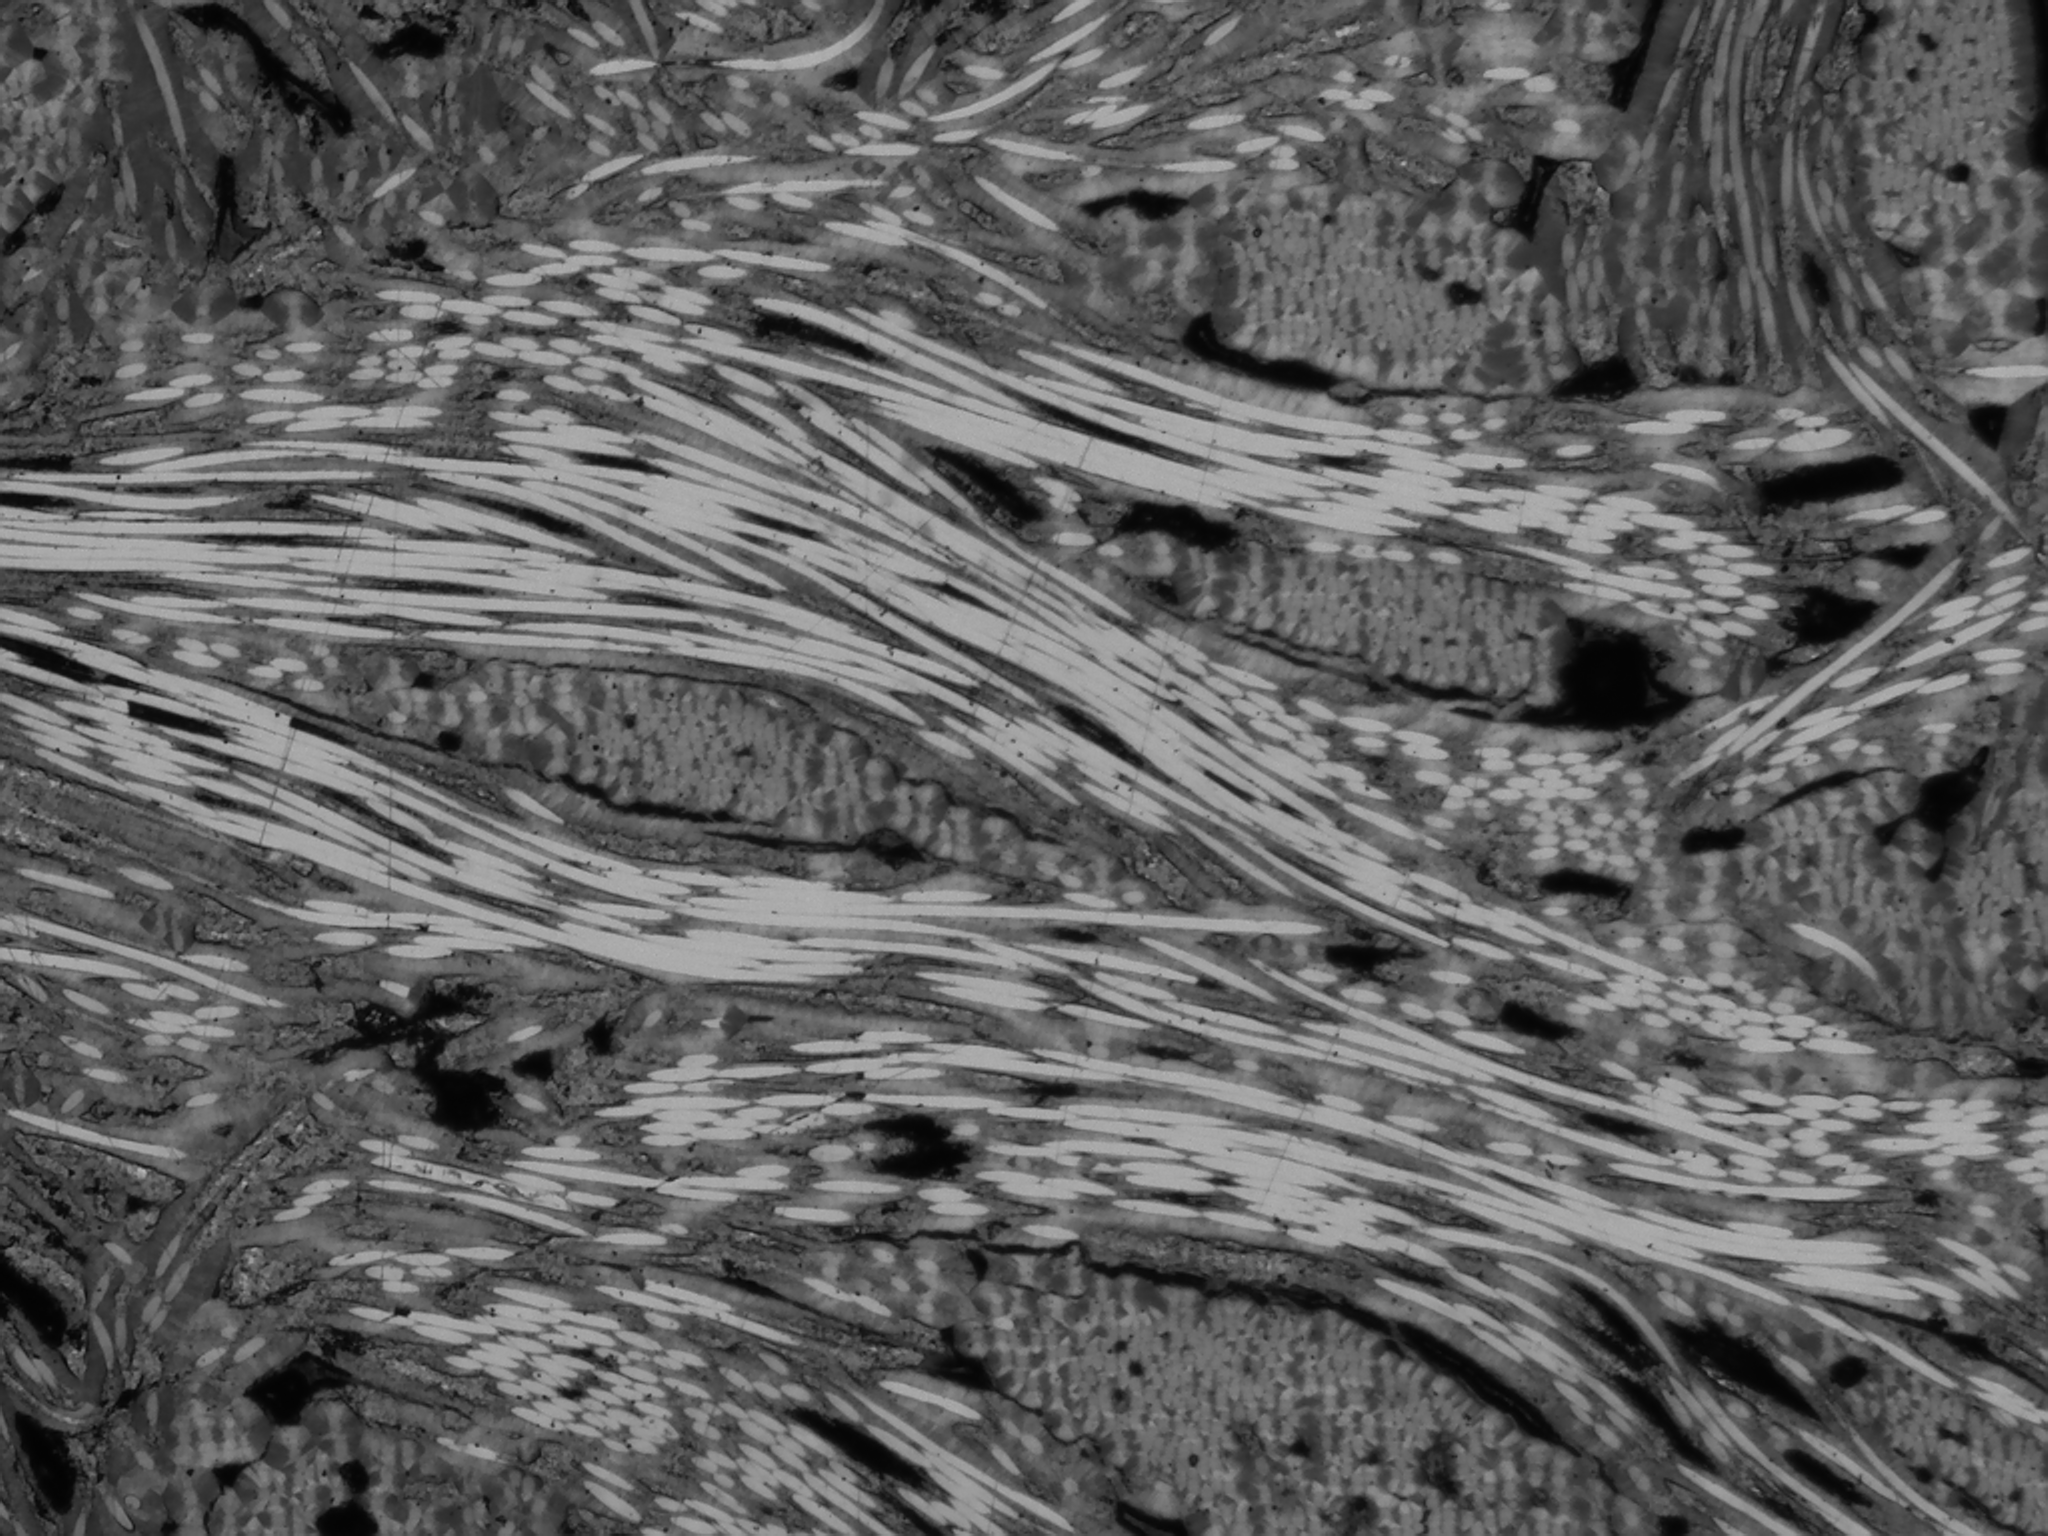
\includegraphics[width=0.8\textwidth]{figures/45_0.68um.png}
    \caption{Image microscopique du composite C/C obtenue au LCTS, avec une résolution de 0.68 $\mu$m/pixel, montrant la diversité de la microstructure du matériau.}
    \label{fig:img_original}
\end{figure}

Cette image présente une microstructure complexe, avec des fibres de carbone enrobées de matrice avec des porosités de tailles variées. Sur cette image à l'échelle mésoscopique, on observe des amas des fibres dans des directions variées, avec des fibres parfois coupées transversalement, d'autres longitudinalement, et des fibres partiellement fusionnées. Cela illustre aussi la polarisation de l'image, avec la couleur des fibres variant selon leur orientation. La détection des fibres dans ce contexte est un défi majeur, nécessitant des méthodes robustes capables de gérer la diversité des formes et des textures présentes. La première partie de l'étude porte surtout sur les amas de fibres coupées transversalement, qui sont plus petits et plus sombres sur l'image.

\subsection{Approche classique : transformée de Hough}

La première approche développée pour la détection des fibres dans les images microscopiques est basée sur la transformée de Hough pour cercles, qui est une technique classique de vision par ordinateur adaptée à la détection d'objets circulaires. Cette méthode repose sur l'hypothèse que les fibres apparaissent comme des cercles dans les images, ce qui est une approximation raisonnable pour les fibres coupées transversalement. Le processus de détection (\texttt{traitement.py}) comprend plusieurs étapes :

\begin{enumerate}
    \item \textbf{Prétraitement} : Conversion de l'image couleur en niveaux de gris, suivie d'un filtrage gaussien avec un noyau $9\times9$ et une déviation standard de 2 pixels pour réduire le bruit tout en préservant les contours des fibres.

    \item \textbf{Détection de cercles} : Utilisation de la transformée de Hough pour cercles via la fonction \texttt{cv2.HoughCircles} d'OpenCV. Les paramètres sont ajustés pour détecter des cercles avec des rayons compris entre 40 et 50 pixels, correspondant à la taille des fibres dans l'image.

    \item \textbf{Validation et sauvegarde} : Les cercles détectés sont validés visuellement et leurs paramètres (coordonnées $x$, $y$ du centre et rayon) sont sauvegardés dans le fichier \texttt{cercles.txt}.
\end{enumerate}

Pour une image prise au LCTS,la détection automatique grâce à la transformée de Hough a permis d'identifier 28 fibres :

\begin{figure}[H]
    \centering
    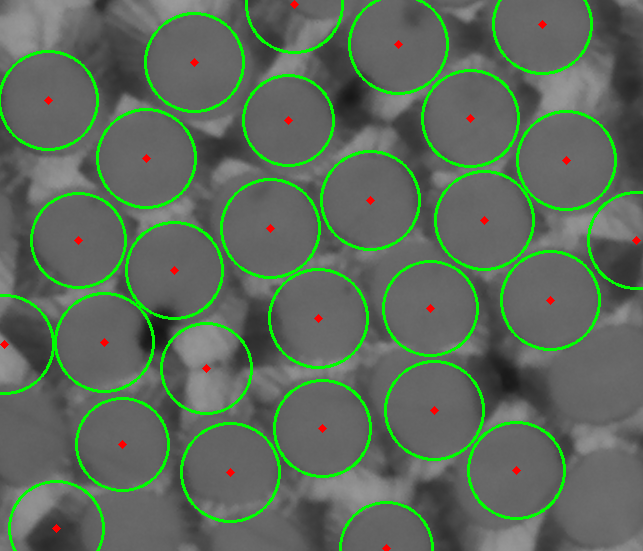
\includegraphics[width=0.55\textwidth]{figures/detected_circles.png}
    \caption{Détection automatique des 28 fibres (cercles verts avec centres rouges) sur l'image du composite}
    \label{fig:detected_circles}
\end{figure}

La détection s'avère satisfaisante, avec une localisation précise des centres et des rayons des fibres. Au niveau des bords de l'image, certaines fibres sont partiellement visibles, ce qui entraîne une détection incomplète. On compte environ 5 faux positifs et 2 faux négatifs. En retirant les détections de bord, on obtient 1 seul faux positif. Même si les cercles détectés ne correspondent pas parfaitement à la forme réelle des fibres (qui peuvent être légèrement elliptiques ou présenter des irrégularités), ils fournissent une approximation suffisante pour la génération du maillage et la simulation numérique ultérieure.

\subsubsection{Génération depuis la détection Hough}

La génération automatique du maillage constitue l'étape intermédiaire cruciale reliant l'analyse d'image à la simulation numérique. Le script Python \texttt{maillage.py} lit les coordonnées des fibres détectées dans le fichier \texttt{cercles.txt} et crée un fichier géométrique Gmsh (.geo) décrivant la géométrie du VER. Le processus comprend la lecture des données, la gestion des systèmes de coordonnées (OpenCV : origine en haut à gauche ; Gmsh : origine en bas à gauche), la construction géométrique des surfaces, l'assignation des tags physiques et l'optimisation du paramètre de raffinement (\texttt{lc}).

\begin{figure}[H]
    \centering
    
\includegraphics[width=0.6\textwidth]{figures/mesh.png}
    \caption{Maillage généré automatiquement depuis la détection Hough : 14\,240 éléments triangulaires avec fibres (noir) dans matrice (bleu)}
    \label{fig:mesh}
\end{figure}

Le maillage final comprend 6\,673 nœuds et 14\,240 éléments triangulaires, avec des contours nets pour les fibres et un maillage uniforme pour la matrice. Le maillage est de bonne qualité, avec des éléments bien proportionnés et une bonne résolution autour des fibres. 

% -------------------------------------------------------------------
\subsubsection{Limites de l'approche classique et motivation pour le deep learning}
% -------------------------------------------------------------------

L'approche par transformée de Hough repose sur une hypothèse forte : les fibres sont approximativement circulaires et leurs rayons sont connus à l'avance (40/50 pixels dans l'image considérée). Cette contrainte paramétrique rend la méthode sensible aux variations d'éclairage, aux fibres partiellement visibles en bordure de champ, et surtout à la présence de porosités ou d'autres hétérogénéités dans la matrice. \\

La transformée de Hough ne fournit qu'une détection binaire fibre/non-fibre et ne permet pas de segmenter les porosités. De plus, pour des images présentant des fibres à géométrie irrégulière, des sections elliptiques dues à l'angle de coupe, ou des amas de fibres jointives, la robustesse de la méthode géométrique se dégrade fortement. Dans les images obtenues au LCTS, on observe une grande diversité de formes et de textures, avec des fibres parfois partiellement fusionnées, des porosités de tailles variées, et un contraste non uniforme. Parfois, les fibres sont plus fonçées que la matrice selon la polarisation, mais dans d'autres cas, les fibres peuvent être plus claires ou présenter des variations de luminosité. \\

En particulier, dans le cas transversal, la détection des fibres est particulièrement difficile à cause de la polarisation de l'image, qui présente une interphase fibre-matrice qui se mélange avec les fibres elles-mêmes. D'autres méthodes ont été testées, comme le seuillage adaptatif, la détection de contours via Watershed ou filtre Otsu, mais elles ont également montré des performances limitées en raison de la complexité de la microstructure et du contraste non uniforme. Une méthode d'apprentissage non supervisée basée sur le clustering (K-means) a également été explorée, mais elle a souffert de la même problématique de contraste et de la difficulté à différencier les fibres des porosités.

\subsection{Approche deep learning : segmentation U-Net}
\label{subsubsec:unet}

\subsubsection{Principe général}

L'apprentissage supervisé est une branche du machine learning où un modèle apprend à faire des prédictions à partir d'exemples étiquetés. Dans le contexte de la segmentation d'images, cela signifie que le modèle reçoit en entrée une image et doit produire une carte de segmentation où chaque pixel est classé dans une catégorie (par exemple, fibre, matrice ou porosité). Cela demande un jeu de données d'entraînement constitué d'images annotées manuellement. Cependant, une fois entraîné, le modèle peut généraliser à de nouvelles images non vues, ce qui en fait un outil puissant pour l'analyse de microstructures complexes \cite{BertoldoUNet}. Les méthodes traditionnelles (Hough, seuillage, etc.) sont souvent limitées par des hypothèses géométriques strictes et ne peuvent pas capturer la diversité des formes et des textures présentes dans les composites réels. En revanche, les réseaux de neurones convolutionnels (CNN) comme le U-Net sont capables d'apprendre des représentations hiérarchiques et de capturer à la fois le contexte global et les détails locaux, à condition d'avoir suffisamment de données d'entraînement et d'une architecture adaptée \cite{HeMultiscale}. \\

Dans un réseau de neurones, les données d'entrée (images) sont transformées à travers une série de couches (convolutions, activations, normalisations, etc.) pour produire une sortie (carte de segmentation). L'entraînement du réseau consiste à ajuster les poids de ces couches pour minimiser une fonction de perte qui mesure l'écart entre les prédictions du modèle et les étiquettes de vérité terrain. Pour entraîner un réseau comme celui-ci, on utilise un ensemble d'images annotées, que l'on divise généralement en un ensemble d'entraînement (pour ajuster les poids) et un ensemble de validation (pour évaluer la performance du modèle sur des données non vues). L'optimisation est souvent réalisée par des algorithmes de descente de gradient, qui mettent à jour les poids du réseau en recherchant le minimum de la fonction de perte. \\

\begin{figure}[H]
    \centering
    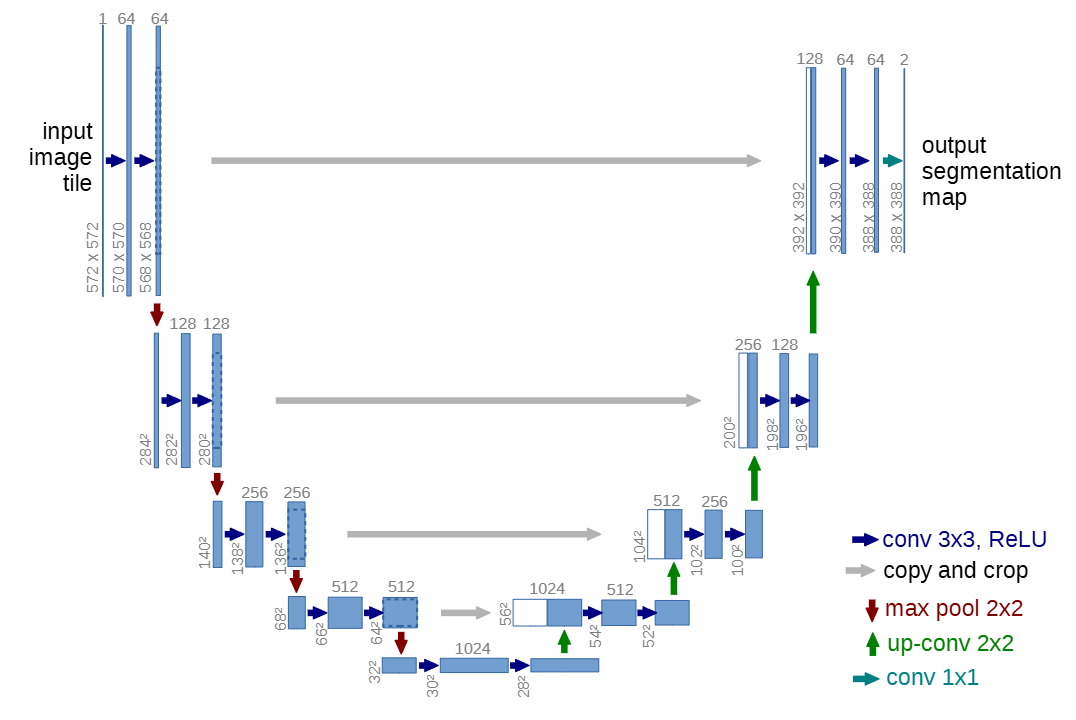
\includegraphics[width=0.7\textwidth]{figures/architecture.png}
    \caption{Architecture du U-Net proposée par Ronneberger et al. (2015) \cite{RonnebergerUNet} pour la segmentation d'images médicales}
    \label{fig:unet_architecture}
\end{figure}

Le U-Net est une architecture spécifique conçue pour la segmentation d'images, proposée initialement par Ronneberger et al. en 2015 \cite{RonnebergerUNet}. Elle est caractérisée par un chemin descendant (encodeur) qui capture le contexte global et un chemin ascendant (décodeur) qui restaure la résolution spatiale, avec des connexions directes (skip connections) entre les deux pour préserver les détails fins. L'approche par U-Net remplace une détection purement géométrique par une segmentation pixel par pixel. Chaque pixel de l'image est classé dans l'une des trois catégories utiles au projet : matrice (classe 0), fibre (classe 1) ou porosité (classe 2). Cette formulation est beaucoup mieux adaptée à une microstructure réelle que la transformée de Hough, car elle ne suppose ni des fibres parfaitement circulaires, ni un rayon connu à l'avance. L'encodeur compresse progressivement l'image en extrayant les features à plusieurs échelles, tandis que le décodeur remonte en résolution pour produire une carte de segmentation fine.

\subsubsection{Architecture du réseau}

L'architecture du U-Net implanté dans ce projet est relativement classique, avec quelques adaptations pour le contexte spécifique de la segmentation de composites. Le réseau prend en entrée une image en niveaux de gris (1 canal) et produit en sortie une carte de segmentation à 3 canaux (un par classe). Ce genre de réseau utilise des blocs de convolution successifs pour extraire les features (textures, formes, contrastes) à différentes échelles, avec des opérations de pooling (sous-échantillonnage) pour réduire la résolution et des convolutions transposées pour la remonter.

Un bloc de convolution double (DoubleConv) représente l'unité de base, composée de deux convolutions successives avec normalisation de batch et activation ReLU. L'encodeur comprend quatre blocs DoubleConv avec des filtres de dimensions croissantes \([32, 64, 128, 256]\), suivis d'un goulot d'étranglement à 512 filtres. Le décodeur remonte par convolutions transposées $2\times2$ en alternance avec des blocs DoubleConv, inversant l'ordre des nombres de filtres. Finalement, une convolution $1\times1$ réduit les 32 canaux de sortie du décodeur à 3 canaux correspondant aux classes. Le réseau apprend ainsi à extraire des features de plus en plus complexes à mesure que l'on descend dans l'encodeur, puis à les combiner pour la segmentation. \\

\subsubsection{Structure du code}

L'implémentation du U-Net est réalisée en Python orienté objet avec PyTorch, une bibliothèque de deep learning populaire pour sa flexibilité et sa facilité d'utilisation. Le code est organisé dans un fichier python \texttt{segmentation.py}, qui contient la définition de l'architecture du réseau, la construction du jeu de données, et les fonctions d'entraînement et d'inférence. Les différentes classes et fonctions sont décrites ci-dessous :

\begin{itemize}
    \item \texttt{DoubleConv} : bloc de base du réseau, composé de deux convolutions successives suivies de normalisation de batch et d'une activation ReLU. Ce bloc est utilisé à la fois dans l'encodeur et le décodeur pour extraire des features à différentes échelles.
    \item \texttt{UNet} : classe principale qui définit l'architecture complète du réseau, avec les couches d'encodeur, de décodeur et les skip-connections. Elle implémente la méthode \texttt{forward} pour la propagation avant des données à travers le réseau. 
    \item \texttt{PatchDataset} : classe dérivée de \texttt{torch.utils.data.Dataset} qui gère la construction du jeu de données à partir des images annotées. Elle extrait aléatoirement des patchs de taille $256\times256$ pixels, applique les augmentations de données, et retourne les paires (image, masque) prêtes pour l'entraînement.
    \item \texttt{train} : fonction qui orchestre le processus d'entraînement du réseau, en itérant sur les époques, en calculant la perte et les métriques de performance, et en ajustant les poids du modèle.
    \item \texttt{predict\_image} : fonction qui applique le modèle entraîné à une nouvelle image, en utilisant une stratégie de fenêtre glissante pour gérer les images de grande taille.
\end{itemize}

La bibliothèque PyTorch prend en charge facilement les architectures de réseaux, gère les opérations de convolution, de normalisation et d'activation, et implémente les boucles d'entraînement avec rétropropagation. Cela permet de se focaliser sur la conception de l'architecture et la gestion du jeu de données. De plus, l'utilisation de GPU avec CUDA est facilitée pour accélérer l'entraînement du modèle, ce qui est crucial pour les réseaux de neurones profonds.

\subsubsection{Construction du jeu de données}

Les données d'apprentissage proviennent des multiples images de microscopie polarisées, que nous avons acquises au LCTS. Parmi ces images, une partie a été annotée manuellement pour créer des masques de vérité terrain, où chaque pixel est étiqueté comme appartenant à la matrice, à une fibre ou à une porosité. Bien que cela paraisse fastidieux à première vue, des outils comme \texttt{Labelme} implémentent des fonctionnalités d'annotation semi-automatique (remplissage intelligent...) et de détection de polygones, ce qui accélère considérablement le processus. Au total, 17 images sur les 46 disponibles ont été annotées, fournissant un jeu de données d'entraînement suffisant pour le réseau. Ces images annotées couvrent une diversité de microstructures, avec des fibres de différentes tailles, des porosités variées et des contrastes différents, ce qui est crucial pour la généralisation du modèle. \\

\begin{figure}[H]
    \centering
    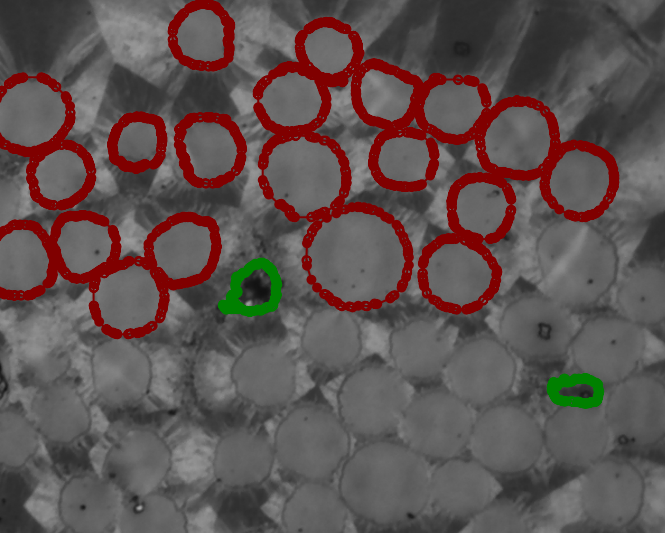
\includegraphics[width=0.6\textwidth]{figures/exemple_annotation.png}
    \caption{Exemple d'image en train d'être annotée avec Labelme : Les polygones rouges représentent les fibres annotées, les polygones verts représentent les porosités.}
    \label{fig:annotated_image}
\end{figure}

Labelme permet d'obtenir le fichier JSON d'annotation, qui est ensuite converti en masque de segmentation binaire (matrice de même taille que l'image, avec des valeurs entières correspondant aux classes). Ces masques sont stockés dans le dataset sous la forme \texttt{label.png} associé à chaque image d'entrée \texttt{image.png}. Ce sont ces paires (image, masque) qui sont utilisées pour entraîner le U-Net à apprendre à segmenter les images de microscopie en trois classes distinctes. Seulement, 17 images annotées pour la segmentation d'images complexes est faible, et peut mener à un sur-apprentissage, c'est-à-dire que le modèle apprend à mémoriser les images d'entraînement plutôt qu'à généraliser à de nouvelles images. C'est pourquoi il est nécessaire dans un premier temps de densifier le jeu de données en découpant les images en patchs plus petits, et dans un second temps d'appliquer des augmentations de données pour simuler une plus grande diversité d'exemples.

\paragraph{Stratégie de patch et densification du jeu.}

La classe \texttt{PatchDataset} extrait aléatoirement de nombreux patchs de taille $256\times 256$ pixels pour chaque image source. Cette stratégie de densification locale permet plusieurs avantages : elle réduit la taille des données chargées en mémoire lors de l'entraînement, elle augmente le nombre d'échantillons effectifs disponibles pour l'optimiseur, et elle force le réseau à apprendre des features invariantes localement. Le code définit \texttt{PATCHES\_PER\_IMAGE = 256}, ce qui signifie que chaque image source contribue $256$ patchs indépendants au jeu de données.

Une séparation 80/20 est ensuite appliquée entre apprentissage et validation : $80\%$ des images sources sont utilisées pour l'apprentissage, $20\%$ pour la validation. C'est une pratique très standard en machine learning, qui permet de mesurer la capacité du modèle à généraliser à des données non vues pendant l'entraînement. La validation est effectuée à l'échelle des images sources, ce qui signifie que les patchs extraits d'une même image ne sont pas partagés entre apprentissage et validation, évitant ainsi les fuites de données.

\paragraph{Augmentation de données.}

L'augmentation des données est une technique cruciale pour améliorer la généralisation du modèle, surtout lorsque le nombre d'exemples annotés est limité. Le principe est simple : on applique de manière aléatoire des transformations géométriques et photométriques aux patchs d'entraînement, créant ainsi des variantes synthétiques de chaque exemple. Cela permet au modèle d'apprendre à être invariant à ces transformations, ce qui est essentiel pour la segmentation de microstructures réelles où les fibres peuvent être orientées de différentes façons, les contrastes peuvent varier, et les artefacts de bruit sont fréquents. Une probabilité d'application de 50\% est généralement utilisée pour chaque transformation, ce qui signifie que chaque patch a une chance égale d'être transformé ou non, créant ainsi une diversité équilibrée dans le jeu de données. Les transformations appliquées sont les suivantes :

\begin{itemize}
    \item Retournements horizontal et vertical,
    \item Rotations ($90^\circ$ ou $[-15^\circ, 15^\circ]$),
    \item Déformations élastiques,
    \item Variations de contraste et correction gamma,
    \item Flou gaussien,
    \item Inversion des niveaux de gris.
\end{itemize}

\vspace{0.2cm}
Toutes ces transformations visent à simuler la diversité des conditions d'imagerie et des microstructures possibles, forçant le réseau à apprendre des features robustes et généralisables. Cela est particulièrement important dans notre cas, où les fibres peuvent être orientées de manière aléatoire, les porosités peuvent varier en taille et en forme, et les images peuvent présenter des artefacts de bruit ou de contraste. Dans ce cas, en comptant l'augmentation des données et le découpage en patch, on obtient, à partir de 17 images annotées, un jeu de données effectif de plusieurs centaines de milliers de patchs.

\subsubsection{Entraînement et inférence}

L'apprentissage du réseau minimise une fonction de perte d'entropie croisée catégorielle, qui compare les logits prédits (sorties non-normalisées du réseau) aux étiquettes de vérité terrain. La perte est définie pour chacun des $256\times256$ pixels de chaque patch, ce qui signifie que le réseau apprend à classer chaque pixel individuellement. \\

La métrique d'intersection over union (IoU) est utilisée pour évaluer la performance du modèle pendant l'entraînement. L'IoU mesure le chevauchement entre la segmentation prédite et la vérité terrain pour chaque classe, et est particulièrement adaptée pour les tâches de segmentation où les classes peuvent être déséquilibrées (par exemple, les porosités peuvent être rares par rapport aux fibres). L'IoU moyen sur les classes présentes dans chaque lot est suivi à chaque époque, permettant de mesurer l'amélioration de la segmentation au fil de l'entraînement. \\

Pour l'entraînement, on parle d'époque pour désigner un passage complet à travers l'ensemble du jeu de données d'entraînement. C'est-à-dire qu'à chaque époque, le modèle ajuste ses poids en fonction de tous les patchs d'entraînement, ce qui permet une convergence progressive vers une solution optimale (qui minimise la fonction de perte). Dans notre cas, on fixe le nombre d'époques à $100$, tout en gardant la possibilité de stopper l'entraînement plus tôt si la validation ne s'améliore plus (early stopping), ce qui permet d'éviter le sur-apprentissage. Pour chaque époque, des données comme la perte d'entropie croisée et l'IoU moyen sont enregistrées pour les ensembles d'entraînement et de validation, ce qui permet de tracer des courbes d'apprentissage et de diagnostiquer le comportement du modèle (par exemple, divergence, sur-apprentissage, sous-apprentissage).

\begin{figure}[H]
    \centering
    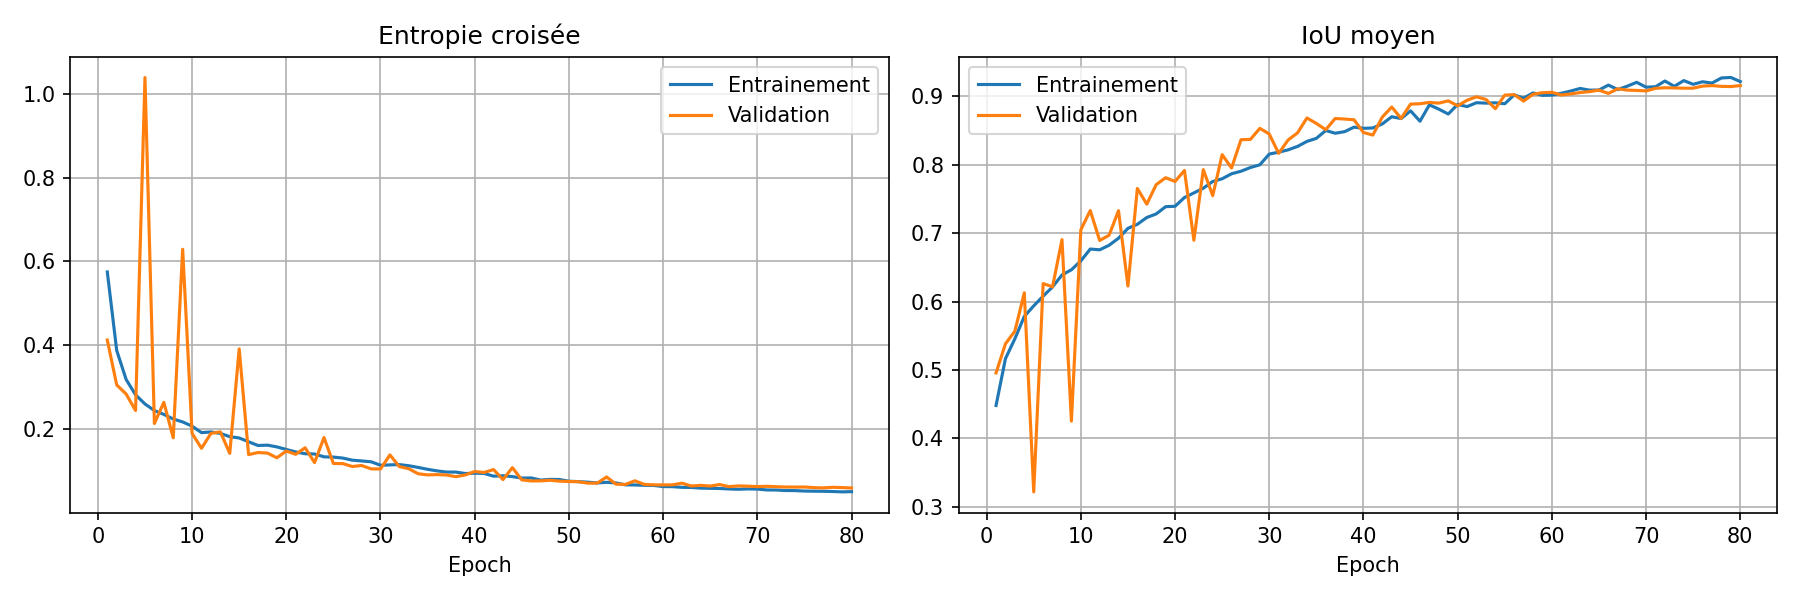
\includegraphics[width=1.05\textwidth]{figures/training_curves.png}
    \caption{Courbes d'entraînement du réseau U-Net. La décroissance de la perte et la stabilisation de l'IoU indiquent que le modèle apprend une segmentation robuste sans divergence entre apprentissage et validation.}
    \label{fig:training_curves}
\end{figure}

L'entraînement à été arrêté à l'époque 80 et a duré environ 30 minutes sur GPU NVIDIA RTX 4060, ce qui est raisonnable pour ce type de projet. Les courbes d'entraînement montrent une décroissance régulière de la perte d'entropie croisée (vers 0.05 environ) et une stabilisation de l'IoU vers 0.92, indiquant que le modèle apprend une segmentation robuste sans divergence entre apprentissage et validation. La partie validation présente plus de variabilité surtout au début de l'entraînement, ce qui est normal compte tenu du nombre limité d'images de validation, mais elle converge vers une performance similaire à celle de l'entraînement. \\

L'early stopping se justifie par le fait que la validation ne s'améliore plus significativement après l'époque 70, ce qui suggère que le modèle a atteint une performance optimale sur les données disponibles. A la fin de cet entraînement, les poids du modèle sont sauvegardés dans un fichier \texttt{unet\_weights.pth}, qui peut être chargé ultérieurement pour faire de l'inférence sur de nouvelles images.

\paragraph{Stratégie d'inférence}

Lors de l'inférence sur une nouvelle image, celle-ci est potentiellement beaucoup plus grande que la taille du patch d'entraînement ($256\times256$). Le code applique donc une stratégie de fenêtre glissante avec vote accumulé (sliding window with voting). Une fenêtre de $256\times256$ est déplacée sur l'image avec un pas (stride) de $192$ pixels, permettant un recouvrement de $64$ pixels entre fenêtres consécutives. Pour chaque fenêtre, le réseau produit un tenseur de probabilités de forme $3 \times 256 \times 256$ (trois canaux pour les trois classes). Ces probabilités sont accumulées dans une carte de votes globale, et le nombre de votes reçu par chaque pixel est enregistré. Finalement, la classe gagnante pour chaque pixel est déterminée par argmax sur la carte de votes normalisée. \\

Cette stratégie a plusieurs avantages : elle réduit les artefacts de bord qui peuvent apparaître quand on traite une image entière d'une fois, elle permet de traiter des images de tailles arbitraires sans modifier le réseau, et le recouvrement et la fusion par vote améliorent la robustesse aux erreurs locales. Différents résultats de prédiction sont présentés pour illustrer la qualité de la segmentation obtenue par le U-Net, avec une distinction claire entre les fibres, la matrice et les porosités.

\begin{figure}[H]
    \centering
    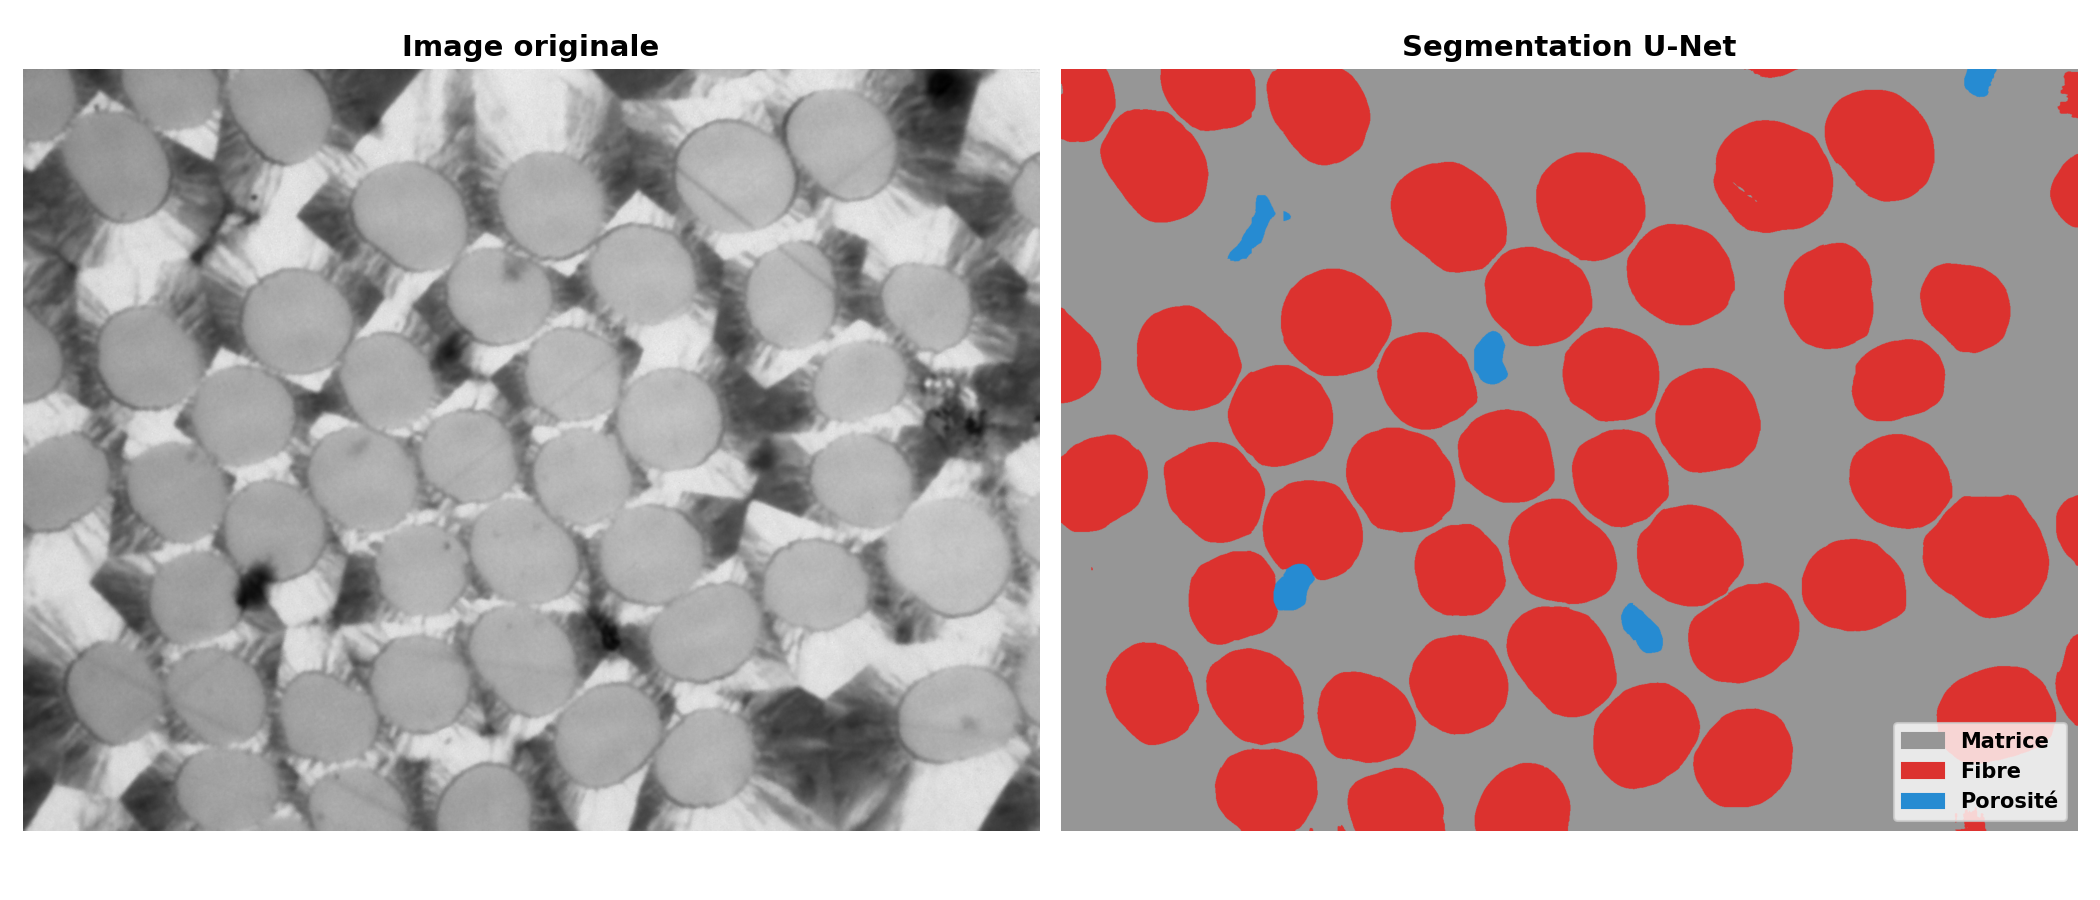
\includegraphics[width=0.85\textwidth]{figures/1_segmented.png}
    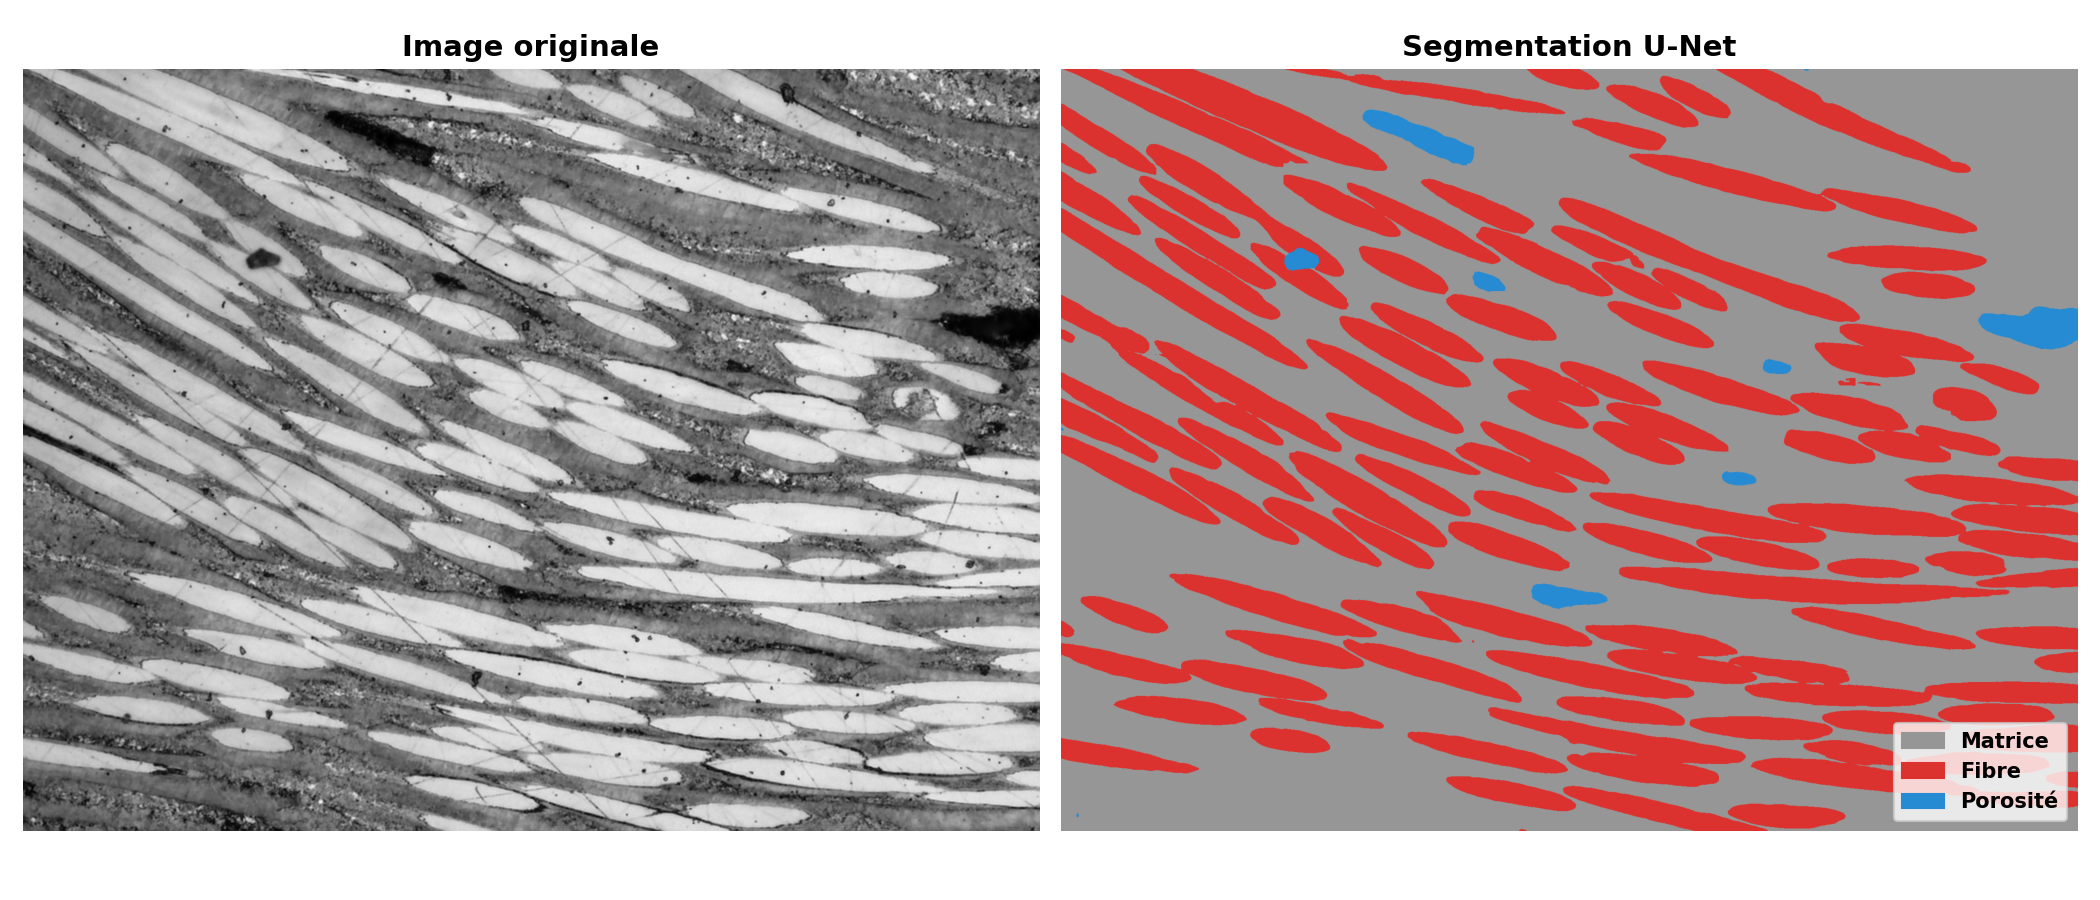
\includegraphics[width=0.85\textwidth]{figures/30_segmented.png}
    \caption{Inférence U-Net sur deux images, avec à gauche l'image originale et à droite la segmentation. La première image montre des fibres circulaires, le second des fibres elliptiques. Les fibres sont en rouge, la matrice en gris, et les porosités en bleu.}
    \label{fig:segmentation_results}
\end{figure}

Que ce soit dans le cas de fibres circulaires ou elliptiques/longitudinales, la segmentation par U-Net est très satisfaisante, avec une délimitation nette des fibres, une bonne distinction entre les classes, et une détection efficace des porosités. La qualité de la segmentation est nettement supérieure à celle obtenue par la transformée de Hough, notamment dans les zones où les fibres sont partiellement visibles ou où les porosités sont présentes. Il n'y a pas besoin de régler manuellement des paramètres de rayon ou de seuil, ce qui rend l'approche plus robuste et plus adaptable à différentes images. \\

La détection de fibres elliptiques/longitudinales est la réelle amélioration, car elle ouvre la voie à l'analyse des propriétés dans la direction longitudinale des fibres. La segmentation est également plus précise pour les fibres partiellement visibles en bordure de champ, qui étaient problématiques pour la transformée de Hough. Même dans le cas transverse, la forme des fibres est bien mieux capturée (pas réellement circulaire) et n'est pas confondue avec l'interphase fibre-matrice. La détection des porosités est très satisfaisante, mais dépend beaucoup de ce que l'on a annoté comme porosité dans le train set. Dans notre cas, nous avons retiré les images avec des fibres arrachées, car trop difficile à annoter avec 3 classes, nous n'avons pas non plus annoté les décollements d'interphase car trop loin pour ce projet, mais cela resterait possible grâce à la puissance du U-Net. Ce modèle échoue cependant pour les images à grande échelle, qui ne s'inscrivent pas dans ce projet qui est à l'échelle des torons.

\paragraph{Comparaison qualitative : Hough vs U-Net.}

Le tableau suivant résume les principales différences entre les approches Hough et U-Net pour la modélisation par traitement d'image du composite C/C.
\begin{table}[H]
    \centering
    \caption{Comparaison des deux approches de traitement d'image pour le composite C/C.}
    \label{tab:comparaison_methodes}
    \begin{tabular}{lcc}
        \toprule
        \textbf{Critère} & \textbf{Hough} & \textbf{U-Net} \\
        \midrule
        Qualité de segmentation & Moyenne & Excellente \\
        Hypothèse géométrique & Cercles de rayon fixe & Aucune \\
        Détection des porosités & Non & Oui \\
        Détection de fibres elliptiques & Non & Oui \\
        Adaptabilité à différentes images & Faible & Élevée \\
        Paramétrisation manuelle & Très élevée & Aucune \\
        Données annotées requises & Non & Oui \\
        Entraînement nécessaire & Non & Oui (30 min sur GPU) \\
        \bottomrule
    \end{tabular}
\end{table}

L'U-Net est supérieur à la transformée de Hough sur tous les critères qualitatifs, mais est beaucoup plus difficile à implémenter, nécessite un jeu de données annoté et un temps d'entraînement. Les mêmes conclusions sont observées dans la littérature, avec d'autres méthodes comme seuillage, variationnelle, watershed... \cite{HeMultiscale}.
\subsection{Génération de maillage à partir de segmentation U-Net}
\label{subsubsec:maillage_unet}

Une fois la segmentation obtenue par le U-Net, il est nécessaire de convertir la carte de segmentation en un maillage exploitable pour les simulations EF. Le script \texttt{mesh.py} réalise cette conversion en plusieurs étapes, depuis le post-traitement du masque jusqu'à la génération du fichier Gmsh (.msh) avec les éléments finis correspondants. Le traitement via Hough permettait d'obtenir une géometrie Gmsh, ce qui permettait de faire rapidement un maillage avec les algorithmes du logiciel. En revanche, la segmentation par U-Net produit un masque pixelisé, qui ne peut pas être directement utilisé pour faire un maillage de qualité. Cela nous force à implémenter un maillage structuré qui se base sur la nature de la segmentation (pixels) plutôt que sur une géométrie continue. \\

Le masque brut obtenu par inférence du U-Net est relu et éventuellement sous-échantillonné par un facteur \texttt{downscale}, où chaque pixel du masque final correspond à un bloc de pixels du masque original. Ce paramètre contrôle le compromis fondamental entre fidélité géométrique et coût computationnel : un sous-échantillonnage agressif réduit le nombre d'éléments et accélère les calculs EF, mais au prix d'une géométrie moins fidèle. Les images ayant des dimensions de l'ordre de $2000\times2000$ pixels, cela amenerait à plus de 4 millions d'éléments à traiter sans downscale. Un deuxième paramètre, \texttt{min\_size}, pilote le nettoyage morphologique appliqué au masque sous-échantillonné. Ce nettoyage est réalisé via \texttt{skimage.morphology} et comprend les opérations suivantes :
\begin{itemize}
    \item Suppression des petits objets (petites porosités ou fragments de fibres).
    \item Comblement des petits trous intérieurs au sein des fibres
    \item Ouverture morphologique spécifique sur les fibres pour éliminer les connexions interfibres.
\end{itemize}

\vspace{0.2cm}
Une fois le masque nettoyé et éventuellement sous-échantillonné, chaque pixel du masque final est ensuite transformé en élément Gmsh. Le format msh 2.2 est généré directement par le code. Deux modes sont proposés : 
\begin{itemize}
    \item Mode \texttt{quad} : un pixel devient un quadrilatère (Q1). Maillage structuré facile à implémenter 
    \item Mode \texttt{tri} : chaque pixel est découpé en deux triangles selon un damier alterné. Deux fois plus d'éléments que le mode quadrilatère, mais meilleure représentation de la géométrie avec optimisation du damier.
\end{itemize}

\vspace{0.2cm}
Les tags physiques (identifiants de région) sont repris directement du masque : chaque pixel reçoit un tag correspondant à sa classe (1 = matrice, 2 = fibre, 3 = porosité). Cela crée automatiquement trois domaines physiques distincts dans le fichier Gmsh, ce qui simplifie ensuite l'affectation des propriétés matériaux dans le solveur EF. Dans toute la suite du code, on privilégie le mode quadrilatère, qui est plus rapide à générer et à traiter que les triangles, et qui est suffisant pour la qualité de segmentation obtenue par le U-Net. Le mode triangulaire structuré est plus coûteux en éléments et nécessite encore plus d'optimisation pour mieux représenter la géométrie. \\

Le passage à une géometrie non structurée de triangles par exemple comme avec Hough nécessite d'implémenter un algorithme de triangulation (Delaunay) à partir de la segmentation, ce qui est extrêmement complexe, car il faut extraire les contours des fibres, les convertir en polygones, gérer les intersections, et faire un maillage de qualité à partir de ces polygones. \\

Le code éléments finis du S7 qui gérait à la base des éléments triangulaires (P1) non structuré, a donc été adapté pour pouvoir gérer des éléments quadrilatères (Q1) structurés, ce qui est plus simple à implémenter et à traiter. Ici, la dimension maximale du maillage est normalisée à 1 unité, ce qui ne prend pas en compte l'échelle physique réelle du composite, ce qui n'est pas un problème comme on travaille en élasticité linéaire. \\

Une pipeline \texttt{main.py} gère l'ensemble du processus : lecture de l'image, segmentation U-Net, post-traitement, génération du maillage Gmsh. Pour l'image de VER présentée en premier dans la figure \ref{fig:segmentation_results}, on affiche sur \texttt{Paraview} le maillage généré pour un downscale de 5 et 15, pour illustrer l'impact du paramètre de sous-échantillonnage sur la fidélité géométrique et le nombre d'éléments générés. 

\begin{figure}[H]
    \centering
    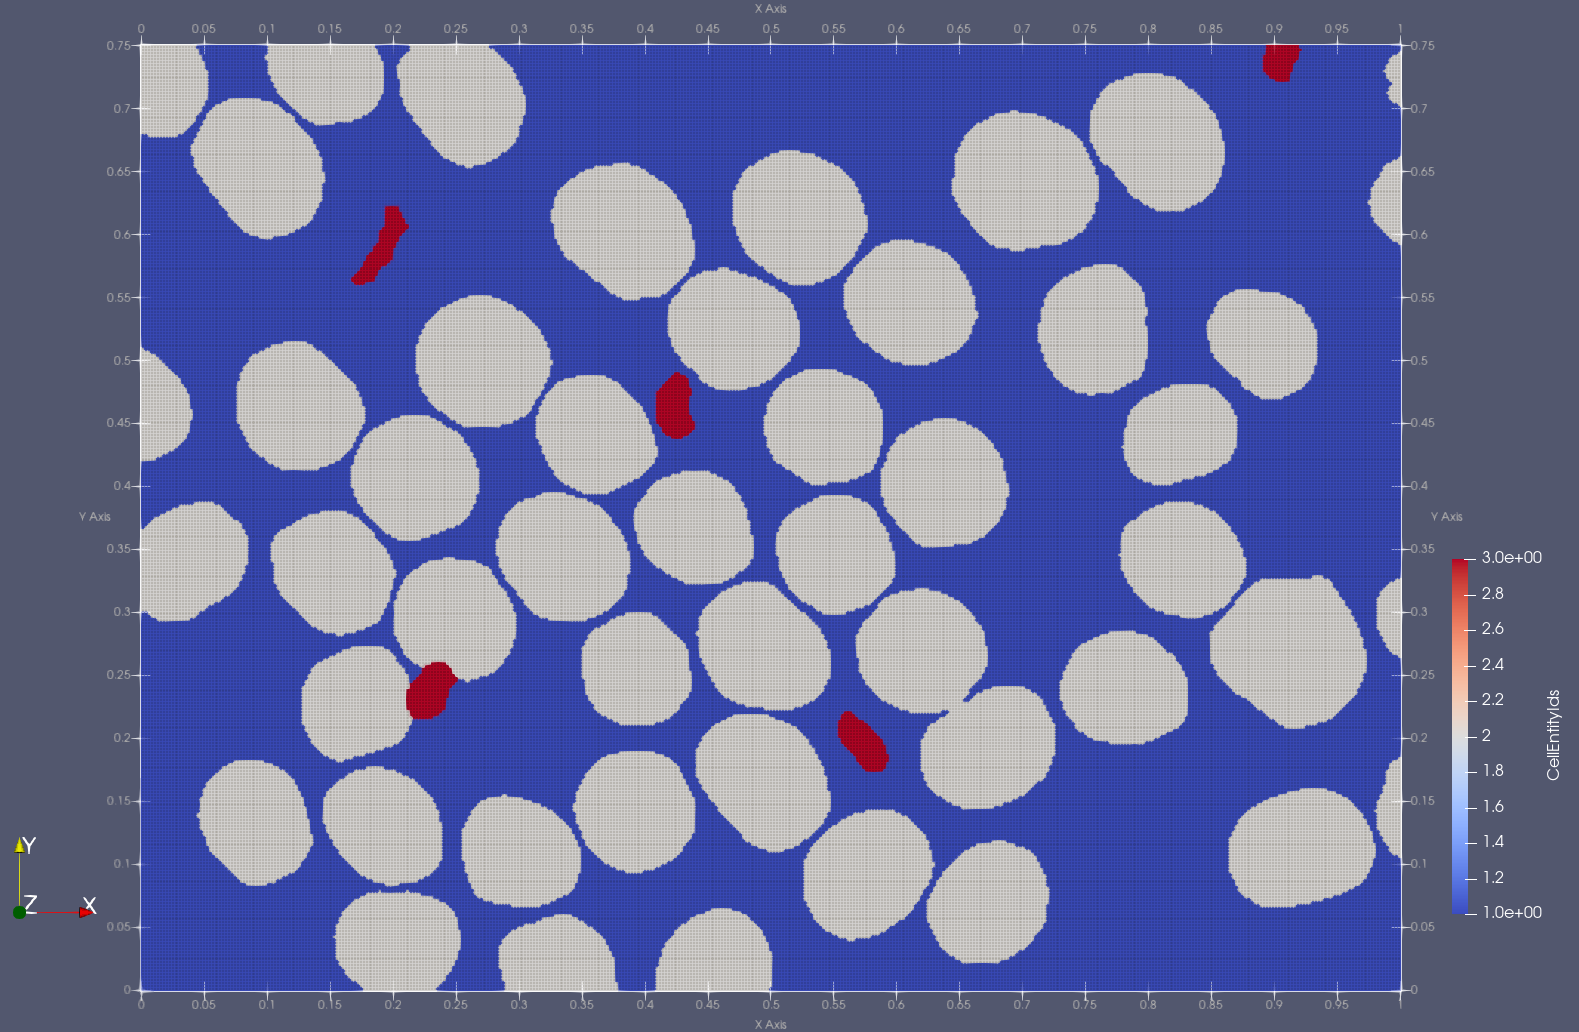
\includegraphics[width=0.49\textwidth]{figures/mesh1_downscale5.png}
    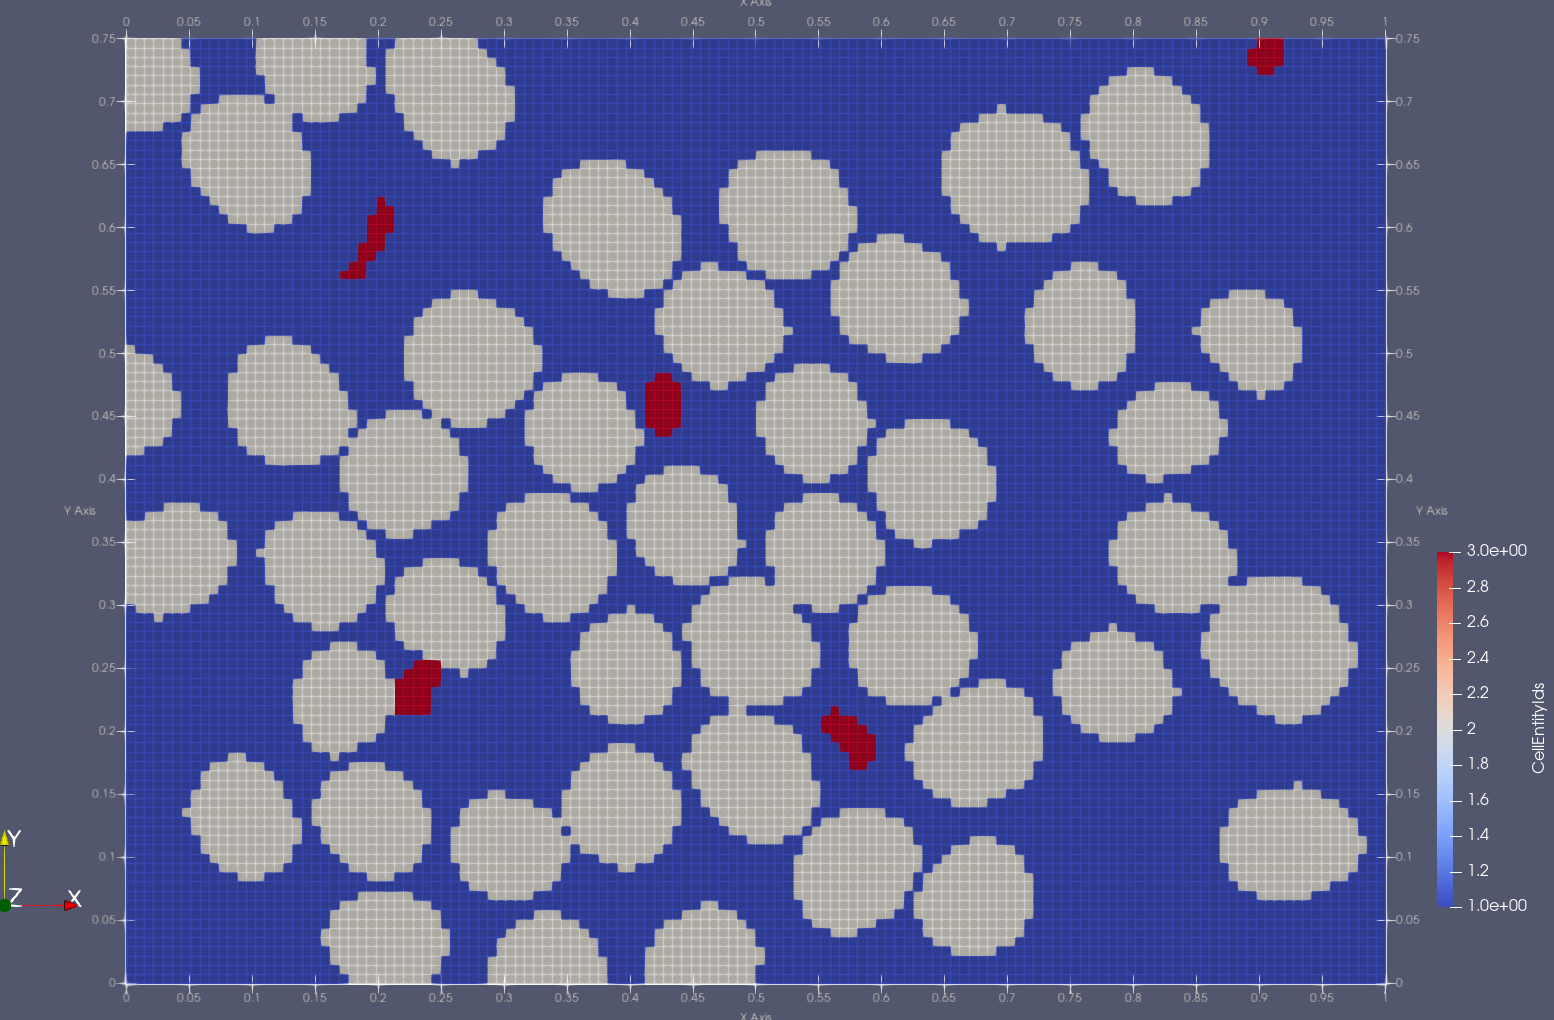
\includegraphics[width=0.49\textwidth]{figures/mesh1_downscale15.png}
    \caption{Maillage généré à partir de la segmentation U-Net pour un downscale de 5 (en haut) et 15 (en bas). 125563 éléments pour le downscale 5, 13872 pour le downscale 15. Tags physiques : 1 = matrice (bleu), 2 = fibre (gris), 3 = porosité (rouge).}
    \label{fig:mesh_downscale}
\end{figure}

Le maillage généré avec un downscale de 15 comporte 13872 éléments quad, tandis que celui avec un downscale de 5 en comporte 125563, soit presque 10 fois plus. On remarque que le maillage avec un downscale de 5 capture beaucoup mieux les détails de la géométrie, notamment les contours des fibres et la séparation inter-fibres, tandis que le maillage avec un downscale de 15 perd une grande partie de la fidélité géométrique. Même avec un nombre conséquent d'éléments, on observe que la géométrie circulaire des fibres n'est pas parfaitement représentée. C'est le principal inconvénient du maillage structuré à partir d'une segmentation pixelisée, l'étude de convergence en maillage sera donc particulièrement importante pour s'assurer que les résultats de la simulation ne sont pas biaisés par la qualité du maillage.

\newpage
\section{Implémentation numérique des éléments finis}
% =============================================================================

\subsection{Méthode des éléments finis pour l'élasticité linéaire}

\subsubsection*{Formulation variationnelle}
La méthode des éléments finis permet de résoudre numériquement des EDP ellipitiques en approximant l'espace des solutions par des fonctions de forme définies localement sur un maillage du domaine. Cette méthode est particulièrement adaptée pour traiter les problèmes d'élasticité linéaire \cite{ZienkiewiczFEM}. Partons de l'équation d'équilibre local dans un domaine solide élastique :

\begin{equation}
\nabla \cdot \boldsymbol{\sigma} + \mathbf{f} = 0 \quad \text{dans } \Omega,
\end{equation}
où $\boldsymbol{\sigma}$ est le tenseur des contraintes, $\mathbf{f}$ représente les forces volumiques (négligées ici), et $\Omega$ est le domaine de la structure. La loi de comportement linéaire relie les contraintes aux déformations par une relation linéaire :

\begin{equation}
\boldsymbol{\sigma} = \mathbf{C}\,\boldsymbol{\varepsilon},
\end{equation}
 
où $\mathbf{C}$ est la matrice de rigidité (ou matrice de comportement) qui dépend des propriétés du matériau, et $\boldsymbol{\varepsilon}$ est le tenseur des déformations, défini à partir du champ de déplacement $\mathbf{u}$ par :
\begin{equation}
\boldsymbol{\varepsilon} = \frac{1}{2}(\nabla \mathbf{u} + \nabla \mathbf{u}^\top).
\end{equation}

Dans un plan d'isotropie, la matrice de rigidité $\mathbf{C}$ est définie par le module de Young $E$ et le coefficient de Poisson $\nu$. \\

On impose des conditions aux limites de Dirichlet (déplacements prescrits) sur une partie du bord $\Gamma_D$ et des conditions de Neumann (forces imposées) sur une autre partie du bord $\Gamma_N$. Sous forme variationnelle, le problème d'élasticité linéaire s'écrit alors : trouver $\mathbf{u} \in V$, tel que pour tout $\mathbf{v} \in V$,

\begin{equation}
\int_\Omega \boldsymbol{\varepsilon}(\mathbf{v}) : \mathbf{C} : \boldsymbol{\varepsilon}(\mathbf{u})\,\mathrm{d}\Omega = \int_{\Gamma_N} \mathbf{v} \cdot \mathbf{f_{surf}}\,\mathrm{d}\Gamma,
\end{equation}

où $V$ est l'espace des fonctions tests (admissibles) et $\mathbf{f_{surf}}$ la force appliquée sur le bord de Neumann. En discretisant l'espace $V$ par des fonctions de forme associées à un maillage d'éléments finis, on obtient un système linéaire de la forme :

\begin{equation}
\mathbf{K}\mathbf{U} = \mathbf{F},
\end{equation}

où $\mathbf{K}$ est la matrice de rigidité globale (creuse, symétrique, définie positive), $\mathbf{U}$ est le vecteur des déplacements nodaux (2 DDL par nœud), et $\mathbf{F}$ est le vecteur des forces nodales. 

\subsubsection*{Assemblage et conditions aux limites}
La matrice $\mathbf{K}$ est assemblée à partir des matrices élémentaires
\[
\mathbf{K}_e = \int_{\Omega_e} \mathbf{B}^\top \mathbf{C}\mathbf{B}\,\mathrm{d}\Omega,
\]
où $\mathbf{B}$ est la matrice de déformation qui relie les déplacements nodaux aux déformations élémentaires, et $\mathbf{C}$ est la matrice constitutive locale. L'assemblage global consiste à sommer les contributions de chaque élément en respectant la connectivité du maillage. Il faut donc avoir une bonne organisation des données, entre les indices locaux (au sein de chaque élément) et les indices globaux (dans le système linéaire). \\

Les conditions aux limites de Dirichlet sont appliquées en modifiant la matrice $\mathbf{K}$ et le vecteur $\mathbf{F}$ pour imposer les déplacements prescrits. Par exemple, pour un nœud $i$ avec un déplacement prescrit $u_i = u_i^*$, on peut remplacer la ligne correspondante dans $\mathbf{K}$ par une ligne de l'identité et ajuster le vecteur $\mathbf{F}$ en conséquence ($F_i = u_i^*$). Les conditions de Neumann sont d'autant plus simples à appliquer, car elles nécessitent simplement d'ajouter les contributions de la force de surface aux entrées correspondantes du vecteur $\mathbf{F}$.

\subsubsection*{Éléments P1}

Dans ce projet, nous avons implémenté deux types d'éléments finis : les triangles linéaires (P1) et les quadrilatères bilinéaires (Q1). Les éléments P1 sont composés de trois nœuds aux sommets du triangle, avec une interpolation linéaire des déplacements. Lorsque le maillage de triangle n'est pas structuré, la matrice de rigidité élémentaire est d'abord calculée pour un triangle de référence, et ensuite transformée pour chaque élément du maillage en fonction de sa géométrie spécifique. On a alors :

\begin{equation}
\mathbf{K}_e = \int_{\Omega_e} \mathbf{B}^\top \mathbf{C}\mathbf{B}\,\mathrm{d}\Omega = \int_{\hat{\Omega}} \mathbf{B}^\top \mathbf{C}\mathbf{B}\,|\mathbf{J}|\,\mathrm{d}\hat{\Omega},
\end{equation}
où $\hat{\Omega}$ est le triangle de référence, $\mathbf{J}$ est la matrice jacobienne de la transformation géométrique, et l'intégration est effectuée numériquement par quadrature de Gauss. La matrice $\mathbf{B}$ est constante sur l'élément, ce qui simplifie le calcul de la matrice de rigidité élémentaire.

\subsubsection*{Éléments Q1}

Dans notre cas, les éléments quadrilatères (Q1) sont majoritairement utilisés, car ils sont plus adaptés au maillage structuré généré à partir de la segmentation U-Net. Les éléments Q1 ont quatre nœuds aux coins du quadrilatère, avec une interpolation bilinéaire des déplacements. La matrice de rigidité élémentaire pour les éléments Q1 est calculée de manière similaire à celle des éléments P1, mais l'intégration doit être effectuée sur le carré de référence $[-1,1]^2$ en utilisant une transformation isoparamétrique. La matrice $\mathbf{B}$ varie linéairement sur l'élément, ce qui nécessite une intégration numérique plus précise (par exemple, quadrature de Gauss à 2 points par direction). \\

\subsubsection*{Résolution du système linéaire}

Le système linéaire résultant est ensuite résolu à l'aide d'un solveur itératif adapté aux systèmes creux, symétriques et définis positifs, tel que le Conjugate Gradient. Un préconditionneur comme le Cholesky incomplet peut être utilisé pour accélérer la convergence. La solution obtenue permet de calculer les déplacements nodaux, à partir desquels on peut dériver les contraintes et les déformations dans chaque élément, et ainsi analyser le comportement mécanique du composite.

\subsection{Architecture du code éléments finis}

Le code éléments finis est implémenté en C++ pour des raisons de performance, avec une organisation modulaire et orientée objet. La programmation orientée objet permet de structurer le code de manière claire et extensible, en encapsulant les différentes fonctionnalités dans des classes dédiées, ce qui est particulièrement important pour un projet de cette envergue. Les différentes parties du code sont présentées ci-dessous, avec une description de leur rôle et de leur interaction.

\subsubsection*{Gestionnaire de configuration}

La classe \texttt{Config} centralise tous les paramètres des simulations :
\begin{itemize}
    \item Type de test (\texttt{testType}) : \textit{``composite''}, \textit{``traction''}, \textit{``flexion''} ou \textit{``shear''}, les trois derniers étant dans des cas homogènes.
    \item Fichier de maillage Gmsh (\texttt{meshFile}) : chemin vers le fichier .msh généré à partir de la segmentation U-Net,
    \item Type d'élément fini (\texttt{elementType}) : P1 (triangle linéaire) ou Q1 (quadrilatère bilinéaire),
    \item Propriétés des matériaux : module de Young $E$, coefficient de Poisson $\nu$, pour matrice, fibres, et éventuellement porosités,
    \item Support optionnel des porosités (troisième matériau si \texttt{hasPores == true}),
    \item Paramètres du solveur : tolérance de convergence, nombre d'itérations maximum, type de préconditionnneur (Cholesky incomplet, diag, id),
    \item Paramètres d'exportation des résultats : format de sortie (Paraview, CSV), etc...
\end{itemize}
\vspace{0.2cm}
Cette architecture permet de charger tous les paramètres depuis un fichier texte simple, typiquement \texttt{config/composite.txt}, sans recompiler le code.

\subsubsection*{Maillage et géométrie}

La classe \texttt{MeshReader} est responsable de l'interprétation des fichiers Gmsh au format 2.2. Elle extrait :
\begin{itemize}
    \item Les positions des nœuds (stockées dans la classe \texttt{Node}),
    \item Les connectivités des éléments (type d'élément selon le code Gmsh : 2 pour P1, 3 pour Q1),
    \item Les tags physiques (identifiants de région, permettant d'associer les différents matériaux aux éléments).
\end{itemize}

\vspace{0.2cm}
Une fonctionnalité importante est que \texttt{MeshReader} identifie aussi les arêtes des bords du domaine, ce qui permet ensuite d'appliquer facilement les conditions aux limites en ciblant tous les nœuds d'une arête ou d'une face donnée (par exemple, \texttt{leftNodes} pour le bord gauche). \\

La classe \texttt{Mesh} encapsule l'ensemble de la structure géométrique et topologique :
\begin{itemize}
    \item Stockage des noeuds, éléments, propriétés (eux mêmes des objets)
    \item Identifications des frontières : \texttt{leftNodes}, \texttt{rightNodes}, \texttt{topNodes}, \texttt{bottomNodes},
    \item Calcul de la fraction volumique par domaine : \texttt{computeVolumeFraction(material)},
    \item Calcul de la longueur caractéristique globale par \texttt{computeCharacteristicLength()},
    \item Méthode \texttt{computeGeometry()} initialise la matrice \texttt{B} et la matrice de rigidité élémentaire \texttt{Ke} pour chaque élément.
\end{itemize}

\vspace{0.2cm}
Une classe \texttt{Node} représente un noeud quelconque, avec ses coordonnées $(x,y)$ et un identifiant global. La classe \texttt{Element} représente un élément fini.
\subsubsection*{Matériaux et propriétés effectives}

La classe \texttt{Material} représente un matériau isotrope. Elle contient :
\begin{itemize}
    \item Module de Young $E$, coefficient de Poisson $\nu$, densité $\rho$,
    \item Matrice de rigidité $\mathbf{C}$, calculée automatiquement lors de la construction via \texttt{computeC()}.
\end{itemize}

\vspace{0.2cm}
La classe \texttt{CompositeMaterial} gère le comportement effectif du matériau composite. Elle stocke :
\begin{itemize}
    \item Pointeurs vers les matériaux constituants (matrice, fibre, porosités), stockage de fractions volumiques.
    \item Stockage des propriétés effectives homogénéisées, actualisées après chaque calcul EF.
    \item Matrices de compliance $\mathbf{S}$ et de rigidité $\mathbf{C}$ de l'homogénéisation, affichage.
\end{itemize}

\vspace{0.2cm}
La méthode \texttt{computeVoigtReussBounds()} calcule les bornes analytiques de Voigt, Reuss, Hill (moyenne arithmétique) et Halpin-Tsai, présentées dans la partie théorique. 

\subsubsection*{Éléments finis}

Les éléments finis sont organisés par une classe de base abstraite \texttt{Element}, avec plusieurs classes filles :
\begin{itemize}
    \item \texttt{ElementP1} : triangle à 3 nœuds avec interpolation linéaire. Chaque élément a 6 DDL (3 nœuds $\times$ 2 DDL par nœud). La matrice $\mathbf{B}$ est constante sur l'élément (elle ne dépend que de la géométrie du triangle), de dimension $3\times 6$.
    \item \texttt{ElementQ1} : quadrilatère à 4 nœuds avec bilinéaire. Il a 8 DDL. L'intégration se fait sur le carré de référence $[-1,1]^2$ par transformation isopapamétrique.
\end{itemize}

\vspace{0.2cm}
Chaque élément stocke la connectivité, son aire, sa matrice \texttt{B}, sa matrice de rigidité élémentaire \texttt{Ke}, et un pointeur vers son matériau associé. La méthode \texttt{compute()} de chaque spécialisation calcule ces quantités à partir de la géométrie et du matériau. Cette classe est la clé de voûte, qui encapsule à la fois la géométrie, l'indexation, les propriétés matérielles, et la formulation variationnelle pour chaque type d'élément.


\subsubsection*{Solveur et assemblage}

La classe \texttt{Solver} orchestre l'assemblage de $\mathbf{K}$ et $\mathbf{F}$, l'application des conditions aux limites, la résolution du système, et le post-traitement. Ses principales méthodes sont :
\begin{itemize}
    \item \texttt{assemble()} : boucle sur tous les éléments, appelle \texttt{compute()} pour chacun, puis ajoute la rigidité élémentaire $\mathbf{K}_e$ aux bonnes positions de la matrice globale $\mathbf{K}$.
    \item \texttt{applyBC()} : modifie $\mathbf{K}$ et $\mathbf{F}$ pour incorporer les conditions de Dirichlet (déplacement imposé) et de Neumann (force imposée). Les conditions de Dirichlet sont appliquées par modification de la matrice vecteur (comme suggéré dans la partie théorique).
    \item \texttt{solveConjugateGradient()} : résout $\mathbf{K}\mathbf{U} = \mathbf{F}$ par gradient conjugué préconditionnné, avec un préconditionnneur sélectionnable (Cholesky incomplet par défaut). La bibliothèque Eigen est utilisée pour la gestion des matrices sparses et la résolution itérative,
    \item \texttt{computeStrainStress()} : après résolution, recalcule $\boldsymbol{\varepsilon} = \mathbf{B}\mathbf{U}_e$ et $\boldsymbol{\sigma} = \mathbf{C}\boldsymbol{\varepsilon}$ pour chaque élément,
    \item \texttt{saveVTK()} : exporte le maillage, les déplacements, les déformations et contraintes au format VTK pour visualisation.
\end{itemize}

\subsubsection*{Cas tests et validation}

Le code possède différents fichiers qui définissent des cas tests spécifiques :
\begin{itemize}
    \item \texttt{test\_traction.cpp}, \texttt{test\_flexion.cpp}, \texttt{test\_shear.cpp} : Cas tests classiques d'élasticité plane pour un matériau homogène isotrope, avec des conditions aux limites spécifiques pour chaque cas : validation du code EF.
    \item \texttt{test\_composite.cpp} : Cas composite général qui effectue les trois chargements de référence sur un VER issu de la segmentation U-Net, et extrait les propriétés homogénéisées.
    \item \texttt{test\_utils.cpp} : Calcule les solutions analytiques, les erreurs, les ordres, export de fichier CSV, etc...
\end{itemize}

L'ensemble du code est orchestré par un fichier \texttt{main.cpp} qui lit la configuration, charge le maillage, initialise les matériaux, et appelle le solveur pour exécuter le cas de test sélectionné. Les résultats sont exportés pour analyse et visualisation. Pour la compilation, un Makefile gère les dépendances et les options de compilation, avec des cibles spécifiques pour chaque cas de test. \\

\texttt{Eigen} est extensivement utilisé pour la gestion des matrices et la résolution linéaire, ce qui simplifie grandement l'implémentation du solveur itératif. Eigen permet aussi d'utiliser directement OpenMP pour le parallélisme, qui est activé pour la résolution du système linéaire avec 16 threads.
\subsection{Validation du code sur matériau homogène}

Dans un premier temps, le code éléments finis est validé sur des cas tests classiques d'élasticité plane pour un matériau homogène isotrope : traction, flexion et cisaillement. Cela permet de vérifier la bonne implémentation de la formulation variationnelle, de l'assemblage, du solveur et surtout des conditions aux limites (point le plus penible). \\

Afin de vérifier à la fois le côté physique et la convergence numérique, nous comparons les résultats numériques à des solutions analytiques disponibles pour ces cas tests. La "simplicité" de ces cas demande d'imposer des conditions aux limites complexes (force répartie comme une Gaussienne, champ de déplacement affine pour le cisaillement), sinon le solveur converge trop rapidement pour observer une courbe de convergence significative. \\

Avec de telles conditions aux limites, il n'y a généralement pas de solution analytique fermée, on choisit donc de calculer une erreur liée à une propriété physique fondamentale : l'énergie de déformation interne :

\begin{equation}
W = \frac{1}{2} \int_\Omega \boldsymbol{\varepsilon} : \mathbf{C} : \boldsymbol{\varepsilon}\,\mathrm{d}\Omega,
\end{equation}

La conservation de l'énergie impose alors que cette énergie de déformation doit être égale à l'énergie induite par les forces appliquées (qui sont connues via les CL). On peut donc calculer une erreur relative sur l'énergie de déformation :

\begin{equation}
\Delta W_{\text{rel}} = \frac{|W_{\text{num}} - W_{\text{CL}}|}{|W_{\text{CL}}|}.
\end{equation}

Avec $W_{\text{num}}$ l'énergie de déformation calculée à partir des résultats numériques (déplacements, déformations, contraintes), et $W_{\text{CL}}$ l'énergie de déformation calculée à partir des conditions aux limites (forces appliquées). Cette métrique sera principalement utilisée pour évaluer la convergence du code éléments, elle est particulièrement robuste car elle intègre la physique globale du problème, nous comparerons aussi d'autres métriques sur les constantes (E, G, $\nu$) lorsqu'elles sont disponibles. \\

Avec des éléments finis Q1 (ou P1), avec la norme $L^2$, on a les ordres de convergence suivants :
\begin{align}
    | U_h - U |_{L^2} &= \mathcal{O}(h^2) & | \varepsilon_h - \varepsilon |_{L^2} &= \mathcal{O}(h) & | \sigma_h - \sigma |_{L^2} &= \mathcal{O}(h)
\end{align}

$U_h$, $\varepsilon_h$, $\sigma_h$ sont les approximations EF du déplacement, de la déformation et de la contrainte, et $h$ est la taille de maille caractéristique. Cela induit que l'erreur sur l'énergie de déformation doit converger à l'ordre 2, ce qui sera vérifié dans les résultats numériques. Afin de garantir la précision de la validation, nous utilisons le gradient conjugué avec une tolérance fixée à $10^{-12}$ pour exclure toute inférence de l'erreur de résolution du système linéaire sur la convergence observée.

\subsubsection{Traction simple}

Pour le cas de traction simple sur matériau homogène isotrope, la géométrie et les paramètres sont définis comme suit :
\begin{itemize}
    \item Géométrie : domaine carré de taille $L \times H$ avec $L=H=1$.
    \item Taille de maille (convergence): 0.5, 0.25, 0.125, ..., 0.00390625.
    \item Matériau : $E=200$ GPa, $\nu=0.3$. 
    \item Chargement : $F=1\times10^{3}\,$N appliquée distribuée sur le bord droit suivant un profil gaussien en $y$.
\end{itemize}

\textbf{Implémentation des conditions aux limites} : le bord gauche est encastré en déplacement longitudinal, et le noeud central du bord gauche est encastré en déplacement vertical. Cette méthode permet d'éviter les translations rigides et les rotations, tout en permettant une distribution de déplacement plus réaliste que l'encastrement complet du bord gauche. Si l'on encastrait complètement le bord gauche, on obtiendrait des valeurs non physiques, notamment au niveau des coins, ce qui fausserait les résultats futurs.
{\footnotesize
\begin{verbatim}
for (int id : mesh.leftNodes)
    // u_x = 0 sur le bord gauche
    solver.setDirichletBC(nodeId = id, dof = 0, val = 0.0); 
for (int id : mesh.findNodesAtY(mesh.yMax / 2.0))
    solver.setDirichletBC(nodeId = id, dof = 1, val = 0.0); 
// Force gaussienne sur bord droit
applyDistributedForce(solver, mesh, mesh.rightNodes, GaussianProfile(F, ymid, sigma), dof = 0);
\end{verbatim}
}
En l'occurrence $y_\mathrm{mid} = 0.5$ et $\sigma = 0.25$ pour le profil gaussien. Une fois l'essai réalisé, différentes grandeurs sont extraites à partir du champ de déplacement obtenu :
\begin{align}
\sigma_x &= \dfrac{F_{\mathrm{tot}}}{H}, 
& \varepsilon_x &= \dfrac{\bar{u}_{x,\mathrm{right}}}{L}, 
& \varepsilon_y &= \dfrac{\bar{u}_{y,\mathrm{top}} - \bar{u}_{y,\mathrm{bot}}}{H}
\label{eq:traction_metrics}
\end{align}

où $\bar{u}_{x,\mathrm{right}}$ est le déplacement moyen en $x$ sur les noeuds du bord droit et $\bar{u}_{y,\mathrm{top}}$ / $\bar{u}_{y,\mathrm{bot}}$ sont les déplacements moyens en $y$ sur les bords supérieur et inférieur respectivement. Cela permet de rémonter aux propriétés effectives :
\begin{align}
    E_{\mathrm{eff}} &= \dfrac{\sigma_x}{\varepsilon_x}, 
    & \nu_{\mathrm{eff}} &= -\dfrac{\varepsilon_y}{\varepsilon_x}.
\end{align}

L'erreur sur l'énergie de déformation $\Delta W_{\mathrm{rel}}$ est calculée à partir du champ EF :
\begin{itemize}
    \item \texttt{computeStrainStress()} calcule les champs de déformation et de contrainte à partir des déplacements nodaux.
    \item \texttt{computeInternalEnergy()} intègre l'énergie de déformation sur tout le domaine à partir du champ de déformation et de la matrice de rigidité.
    \item \texttt{computeExternalWork()} intègre le travail des forces appliquées à partir des conditions aux limites stockées dans le solveur.
\end{itemize}

\subsubsection{Cisaillement pur}
\begin{itemize}
    \item Géométrie et maillage : même que pour la traction simple.
    \item Matériau : $E=200\,$GPa, $\nu=0.3$.
    \item Chargement : traction tangente appliquée sur le bord supérieur suivant un profil gaussien en $x$, résultante totale $F$ prescrite dans la configuration.
\end{itemize}

\textbf{Conditions aux limites :} la face inférieure (\texttt{mesh.bottomNodes}) est encastrée ($u_x$ = $u_y$ = 0). La force répartie tangente est appliquée sur \texttt{mesh.topNodes} (composante 0) avec profil gaussien centré en $x_{\mathrm{mid}}$. Cela permet d'obtenir un champ de déplacement affine en $x$ (champ de cisaillement pur) qui est plus difficile à reproduire pour le solveur que les profils de déplacement plus simples des cas de traction et flexion, ce qui rend la validation plus robuste. Une fois le champ de déplacement obtenu, on peut calculer les grandeurs suivantes :

\begin{align}
\gamma_{\mathrm{eff}} &= \dfrac{\bar{u}_{x,\mathrm{top}}}{H}, & \tau_{\mathrm{mean}} &= \dfrac{F_{\mathrm{tot}}}{L}, \\
G_{\mathrm{eff}} &= \dfrac{|\tau_{\mathrm{mean}}|}{|\gamma_{\mathrm{eff}}|}
\end{align}

où $\bar{u}_{x,\mathrm{top}}$ est le déplacement moyen en $x$ sur les noeuds supérieurs, $\gamma_{\mathrm{eff}}$ est la déformation de cisaillement effective, $\tau_{\mathrm{mean}}$ est la contrainte de cisaillement moyenne, et $G_{\mathrm{eff}}$ est le module de cisaillement effectif. Le module effectif peut être comparé à la solution analytique pour un matériau homogène isotrope : $G = \dfrac{E}{2(1+\nu)}$, en plus de l'erreur sur l'énergie de déformation $\Delta W_{\mathrm{rel}}$.

\subsubsection{Flexion}
Géométrie : poutre de rapport longueur/hauteur $10\times1$ (longueur 10, hauteur 1). Maillages et paramètres :
\begin{itemize}
    \item Modules de maillage : 0.1, 0.05, 0.025, ..., 0.00078125.
    \item Matériau : $E=200\,$GPa, $\nu=0.3$.
    \item Chargement : traction linéaire (profil en $y$) sur le bord de droite, résultante totale $F = -1\times10^{3}\,$N.
\end{itemize}

\textbf{Conditions aux limites :} l'extrémité gauche est encastrée ($u_x = u_y = 0$ pour \texttt{mesh.leftNodes}). Une condition supplémentaire est imposée pour bloquer le déplacement vertical en un point médian afin d’éviter les modes rigides. La force répartie sur le bord droit est appliquée dans la direction horizontale (composante 0) selon un profil gaussien centré.

Une fois le champ de déplacement obtenu, on évalue l’erreur en norme $L^2$ en comparant la solution numérique à une solution analytique issue de la théorie des poutres d’Euler-Bernoulli. Le chargement est ramené à une résultante $F_{\mathrm{eq}}$ et un moment $M_{\mathrm{eq}}$. L’erreur $L^2$ est ensuite calculée via \texttt{solver.computeL2Error(exact)}.

\subsubsection{Résultats de la validation}

La validation est donc effectuée en comparant les résultats numériques à des solutions analytiques pour les trois cas tests, en évaluant l'erreur relative sur l'énergie de déformation $\Delta W_{\mathrm{rel}}$ et d'autres métriques physiques (E, G, $\nu$) lorsque cela est possible. Cela est réalisé pour différentes tailles de maillage $h$, afin d'observer la convergence du code éléments finis. Les tableaux pour chaque cas test sont présentés en annexe pour ne pas alourdir le rapport, mais les résultats montrent une convergence claire de l'erreur relative sur l'énergie de déformation à l'ordre 2, ce qui confirme la bonne implémentation de la méthode des éléments finis pour l'élasticité linéaire. De plus, les propriétés effectives calculées (E, G, $\nu$) convergent également vers les paramètres du matériau homogène, ce qui renforce la validation du code. Enfin, les temps de calcul sont également reportés pour chaque maillage, montrant une augmentation significative avec la taille du maillage (92s en flexion pour 163840 éléments). La figure ci-dessous résume les résultats de convergence, en montrant l'évolution de l'erreur relative sur l'énergie de déformation $\Delta W_{\mathrm{rel}}$ en fonction de la taille de maille $h$ pour les trois cas tests, avec des régressions linéaires en échelle log-log pour vérifier les ordres de convergence attendus.


\begin{figure}[H]
    \centering
    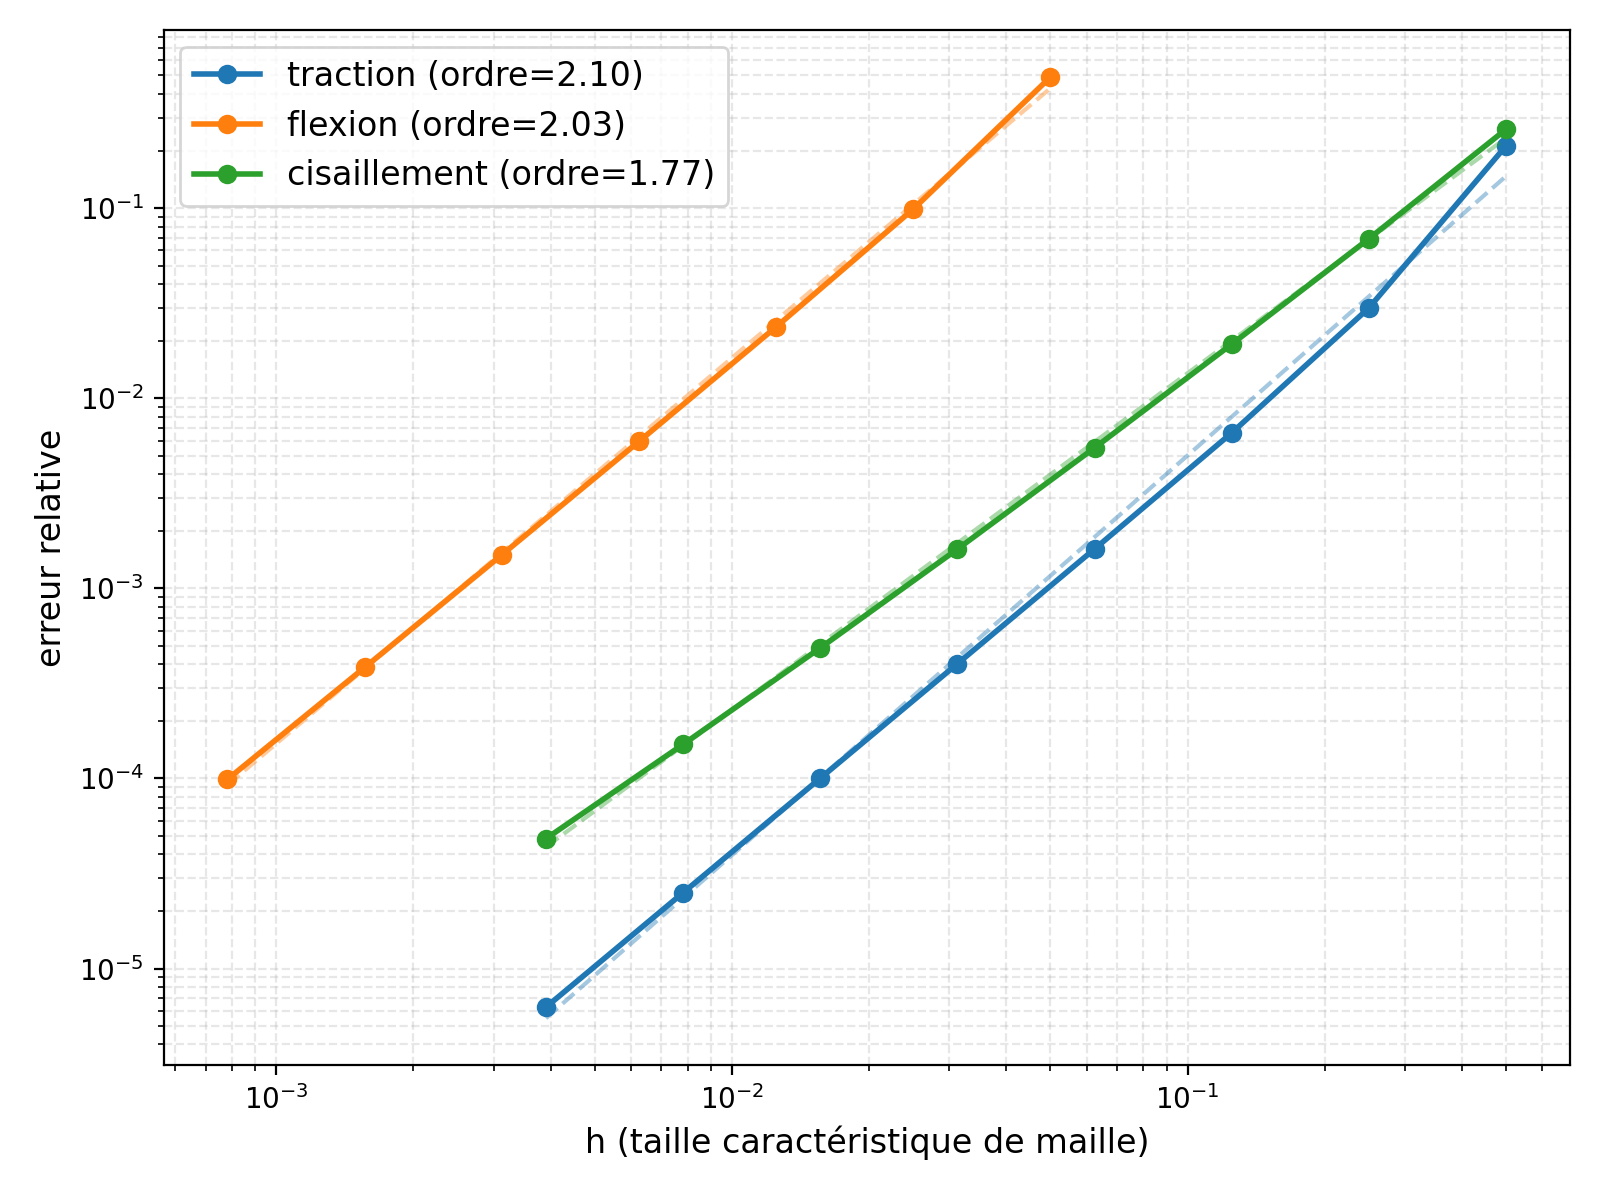
\includegraphics[width=0.70\textwidth]{figures/validation_convergence.png}
    \caption{Synthèse des résultats de convergence pour les trois cas tests (traction, flexion, cisaillement). $\Delta W_{\mathrm{rel}}$ en fonction de la taille de maille $h$ en échelle log-log. Les régressions linéaires sont affichées en couleur clair en pointillés, avec la pente en légende.}
    \label{fig:validation_convergence}
\end{figure}

Globalement, un ordre de convergence de 2 est observé pour l'erreur relative sur l'énergie de déformation, ce qui est conforme à la théorie pour des éléments finis linéaires (P1 ou Q1) en norme $L^2$. Les erreurs relatives ont des valeurs raisonnables, allant de $2\times10^{-1}$ pour les maillages les plus grossiers à $6\times10^{-6}$ pour les maillages les plus fins, ce qui confirme la robustesse et la précision du code éléments finis implémenté. Le cas de flexion montre une convergence plus lente que les autres cas, ce qui est attendu en raison de la nature plus complexe du champ de déplacement et des contraintes dans ce cas, bien que l'ordre de convergence reste globalement proche de 2. Ces résultats valident la bonne implémentation de la méthode des éléments finis pour l'élasticité linéaire, et permettent de passer à l'étude du cas composite avec confiance dans les résultats numériques, et les conditions aux limites appliquées.

\section{Homogénéisation numérique dans le plan transverse}

Nous étudions désormais le comportement effectif du composite C/C dans le plan transverse, c'est-à-dire perpendiculaire à l'axe des fibres. Le matériau est alors supposé isotrope dans ce plan, avec des propriétés effectives à déterminer par homogénéisation numérique. Le maillage est généré à partir de la segmentation U-Net, qui fournit une géométrie réaliste du VER du composite, en omettant les porosités dans un premier temps. Les propriétés effectives sont extraites avec une démarche similaire aux cas tests de validation, en appliquant des chargements de traction dans les deux directions, et un chargement de cisaillement pur, pour calculer l'intégralité des propriétés effectives dans ce plan : $E_{11}$, $E_{22}$, $\nu_{12}$, et $G_{12}$. \\ 

\subsection{Paramètres de la simulation}
Pour le choix des propriétés isotropes individuelles des fibres et de la matrice, nous avons utilisé des données issues de la littérature sur les composites C/C type CVI (Chemical Vapor Infiltration) à base de fibres de la famille PAN et de matrices pyrocarbone. L'article de Ozcan et al. (2009) \cite{OzcanCC} fournit des valeurs typiques pour les modules d'Young de la fibre et matrice après traitement thermique HTT (High Temperature Treatment), de 34 GPa et 12 GPa respectivement. Les coefficients de Poisson sont extraits d'une thèse effectuée au LCTS sur les composites C/C par M. Charron \cite{CharronCC}), qui propose des valeurs pour le module d'Young moins intéressantes pour la simulation (10 et 15 GPa) bien que celle reste dans les mêmes ordres de grandeur que les données d'Ozcan. Les propriétés utilisées pour les simulations sont résumées dans le tableau ci-dessous.

\begin{table}[H]
\centering
\small
\renewcommand{\arraystretch}{1.2}
\begin{tabular}{|c|c|c|}
\hline
\textbf{Phase} & \textbf{$E_T$} & \textbf{$\nu_{TT}$} \\
\hline
Fibre (PAN HTT) & 34 GPa & 0,25 \\
Matrice (Pyrocarbone HTT) & 12 GPa & 0,30 \\
\hline
\end{tabular}
\caption{Propriétés élastiques des constituants du composite pour les simulations.}
\label{tab:properties_composite}
\end{table}

\vspace{0.2cm}
Ces valeurs peuvent sembler faibles, mais la fibre et matrice dans un composite C/C sont très anisotropes, et les propriétés dans le plan transverse sont beaucoup plus faibles que dans la direction longitudinale. Ces valeurs sont aussi cohérentes avec des données expérimentales issues d'autres études comme celle de Maurin et al. \cite{MaurinTransverseCC}, ou encore celle de Guruprasad et al. \cite{GuruprasadNanoindent}. Nous avons volontairement choisi les propriétés de l'article d'Ozcan \cite{OzcanCC} ayant subi un HTT, car cela augmente le contraste entre les propriétés de la fibre et matrice, ce qui rend l'étude du composite plus intéressante (sans HTT, module similaire de 18 GPa, pas de comparaison possible). \\

Pour les paramètres de la simulation, nous utilisons le gradient conjugué préconditionné avec un préconditionneur de Cholesky incomplet, pour les paramètres du solveur, nous fixons :
\begin{itemize}
    \item Tolérance de convergence : \texttt{tol} = $10^{-6}$
    \item Nombre d'itérations maximum : \texttt{maxIter} = 4000
    \item Nombre de threads : 16
\end{itemize}

\vspace{0.2cm}
La tolérance est standard pour un problème complexe comme celui-ci, et le nombre d'itérations maximum permet de garantir la convergence même pour des maillages très fins avec des centaines de milliers d'éléments.

\subsection{Méthode d'extraction des propriétés effectives}

Afin d'extraire les propriétés effectives du composite, nous appliquons trois types de chargements de référence sur le VER :
\begin{itemize}
    \item Traction dans la direction $x$ (Traction 1) : permet d'extraire $E_{11}$ et $\nu_{12}$,
    \item Traction dans la direction $y$ (Traction 2) : permet d'extraire $E_{22}$ et $\nu_{21}$,
    \item Cisaillement pur : permet d'extraire $G_{12}$.
\end{itemize}

Ces chargements sont appliqués de manière similaire aux cas tests de validation, avec des conditions aux limites similaires concernant les encastrements. Pour les forces réparties, il n'y a pas besoin d'appliquer un profil Gaussien car nous ne sommes plus dans une démarche de validation, des forces réparties uniformes sont appliquées sur les bords du VER pour induire les champs de déplacement nécessaires à l'extraction des propriétés effectives. \\
\subsubsection*{Traction 1}

Comme pour la traction simple dans la validation, différents paramètres sont utilisés :
\begin{itemize}
    \item Maillage : VER issu de la segmentation U-Net, domaine $L \times H$, taille de maille caractéristique $h$.
    \item Matériaux : fibre et matrice (isotropes dans le plan) \ref{tab:properties_composite}.
    \item Conditions aux limites : bord gauche encastré ($u_x = 0$), noeud médian du bord gauche avec $u_y = 0$, force répartie uniforme sur le bord droit dans la direction $x$ (F = 1e6 N)
\end{itemize}

La démarche d'extraction des propriétés effectives est similaire à celle de la traction simple dans la validation :

\begin{align}
    E_{11} &= \dfrac{\sigma_x}{\varepsilon_x},
    & \nu_{12} &= -\dfrac{\varepsilon_y}{\varepsilon_x}.
\end{align}

\subsubsection*{Traction 2}

Le deuxième cas de traction est similaire au premier, mais avec les conditions aux limites adaptées pour appliquer une traction dans la direction $y$ :
\begin{itemize}
    \item Bord inférieur encastré ($u_y = 0$), noeud médian du bord inférieur avec $u_x = 0$, force répartie uniforme sur le bord supérieur dans la direction $y$ (F = 1e6 N).
\end{itemize}

Les propriétés effectives sont extraites de manière similaire :
\begin{align}
    E_{22} &= \dfrac{\sigma_y}{\varepsilon_y},
    & \nu_{21} &= -\dfrac{\varepsilon_x}{\varepsilon_y}.
\end{align}
\subsubsection*{Cisaillement pur}    

Le cas de cisaillement pur est similaire à celui de la validation, avec des conditions aux limites adaptées pour appliquer une traction tangente sur le bord supérieur :
\begin{itemize}
    \item Bord inférieur encastré ($u_x = u_y = 0$), La force répartie tangente est reproduite en imposant une condition du champ de cisaillement pur : $u_x = \gamma y$ sur le bord supérieur, avec $\gamma$ la déformation de cisaillement prescrite à partir de la résultante $F$ et de la géométrie du VER.
\end{itemize}

Les propriétés effectives sont extraites de manière similaire :
\begin{align}
    G_{12} &= \dfrac{|\tau_{\mathrm{mean}}|}{|\gamma_{\mathrm{eff}}|}
\end{align}

Dans les trois cas, les champs de déplacement, de déformation et de contrainte sont extraits à partir des résultats numériques pour visualisation VTK, et l'erreur sur l'énergie de déformation est calculée pour évaluer la précision de la simulation. \\ 

Le code effectue les trois simulations de manière successive, en réinitialisant les conditions aux limites et les forces appliquées à chaque fois, tout en exportant les champs de déplacement, de déformation et de contrainte pour chaque cas. Les propriétés effectives sont actualisées au fur et à mesure via l'objet \texttt{CompositeMaterial}. Un fichier CSV est généré à la fin de l'exécution avec les propriétés effectives pour chaque cas, les bornes théoriques (Voigt, Reuss...) et les propriétés du maillage, fraction de fibre, etc... pour analyse et comparaison.

\subsection{Étude de convergence en maillage}

La première étape de l'étude du composite est de vérifier la convergence en maillage des propriétés effectives extraites. En effet, le maillage issu de la segmentation U-Net peut être relativement grossier, et les éléments quad ne prennent pas forcément en compte la géométrie du VER. Pour la géométrie présentée dans la partie U-Net \ref{fig:mesh_downscale}, nous avons généré différents maillages, ayant des tailles caractéristiques allant de 0.0098 (downscale 20) à 0.0015 (downscale 3), ce qui correspond à un nombre d'éléments allant de 7752 à 349184. \\

Le code éléments finis est exécuté pour chaque maillage, en appliquant les trois chargements de référence, et les propriétés effectives sont extraites à chaque fois. Le tableau suivant illustre la convergence des propriétés effectives $E_{11}$, $E_{22}$, $\nu_{12}$, $G_{12}$ en fonction de la taille de maille $h$ et du nombre d'éléments, ainsi que le temps de calcul (seulement celui de la traction 1) pour chaque maillage.

\begin{table}[H]
    \centering
    \setlength{\tabcolsep}{3pt}
    \begin{tabular}{|c|c|c|c|c|c|c|c|c|}
        \hline
        Downscale & $h$ & $N_{\text{elems}}$ & $E_{11}$ (GPa) & $E_{22}$ (GPa) & $G_{12}$ (GPa) & $\nu_{12}$ & $\nu_{21}$ & $t_{\text{cpu}}$ \\
        \hline
        20 & 0,0098 & 7752   & 17,042 & 16,963 & 6,7278 & 0,28858 & 0,28629 & 0,475 \\
        15 & 0,0074 & 13872  & 17,774 & 17,706 & 7,0299 & 0,28645 & 0,28514 & 0,653 \\
        10 & 0,0049 & 31212  & 18,023 & 17,937 & 7,1314 & 0,28654 & 0,28504 & 2,81 \\
        8  & 0,0039 & 49152  & 18,128 & 18,019 & 7,1691 & 0,28612 & 0,28448 & 5,32 \\
        6  & 0,0029 & 87296  & 18,128 & 18,035 & 7,1783 & 0,28643 & 0,28503 & 14,3 \\
        5  & 0,0024 & 125563 & 18,138 & 18,052 & 7,1855 & 0,28651 & 0,28522 & 19,2 \\
        4  & 0,0020 & 196608 & 18,148 & 18,053 & 7,1875 & 0,2866 & 0,28518 & 42,7 \\
        3  & 0,0015 & 349184 & 18,139 & 18,048 & 7,1864 & 0,28677 & 0,28541 & 122 \\
        \hline
    \end{tabular}
    \caption{Résultats de convergence en maillage pour les propriétés effectives du composite.}
    \label{tab:convergence_maillage_composite}
\end{table}

Sans rentrer dans l'analyse physique des résultats, on observe que les propriétés effectives ont des ordres de grandeurs cohérents même pour des maillages très grossiers, ce qui est un bon indicateur de la robustesse du code éléments finis. On observe une convergence très précise à partir d'une taille de maille de 0.0024, ce qui correspond à environ 125000 éléments, ce qui est relativement raisonnable pour une simulation d'homogénéisation numérique. Le temps de calcul pour cette taille de maille (19,2 s) n'étant pas prohibitif, nous choisissons de réaliser l'ensemble des simulations suivantes avec des maillages ayant un raffinement similaire, avec $h$ allant de 0.0024 à 0.003 (downscale à 5 selon la taille de l'image). Concernant le temps de calcul, on observe une augmentation non linéaire du temps de calcul en fonction du nombre d'éléments, ce qui est cohérent avec la complexité algorithmique du solveur de gradient conjugué préconditionné utilisé, pour un downscale supérieur à 5, le temps de calcul devient prohibitif (122s par cas test pour le downscale 3) comparé à la précision obtenue. La figure ci-dessous montre l'évolution des propriétés effectives normalisées (divisées par celles du maillage le plus fin) en fonction de la taille de maille.

\begin{figure}[H]
    \centering
    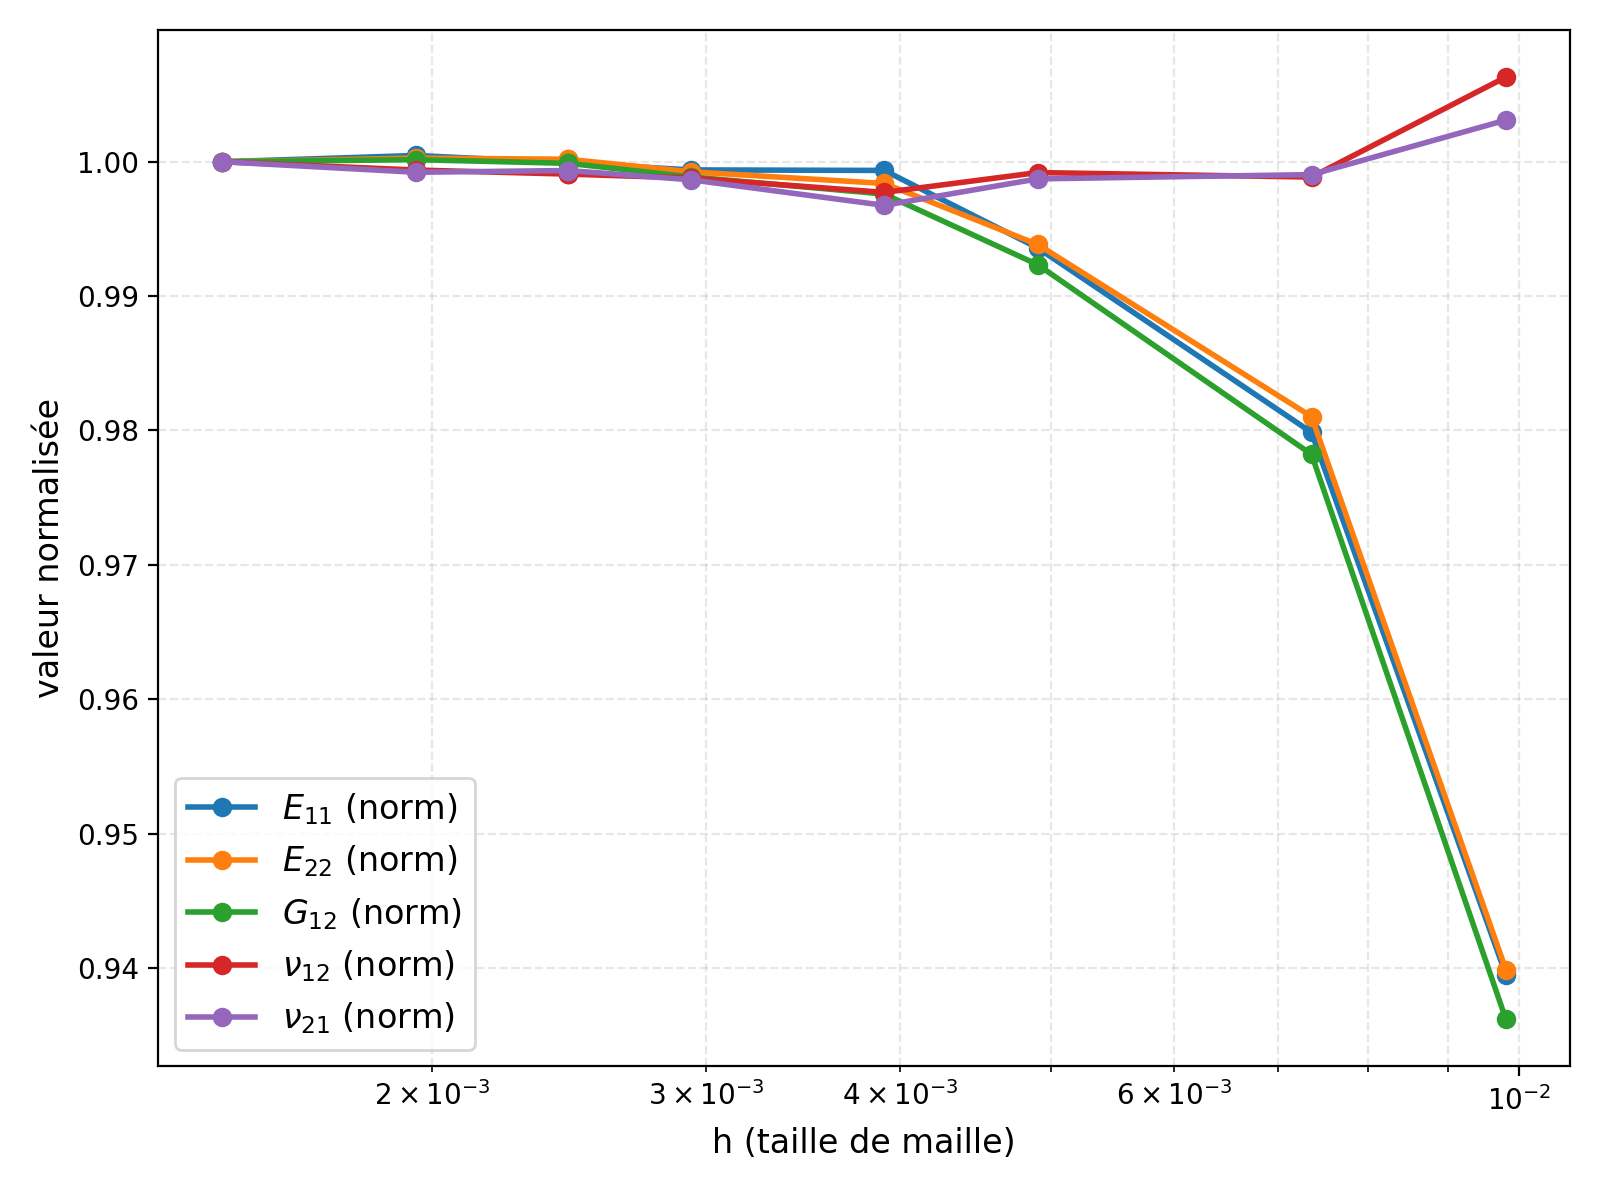
\includegraphics[width=0.75\textwidth]{figures/conv_maillage_proprietes_composite1_vf0.452.png}
    \caption{Étude de convergence en maillage pour le composite, pour les propriétés effectives $E_{11}$, $E_{22}$, $\nu_{12}$, $G_{12}$ qui sont normalisées. Différentes tailles de mailles sont utilisées}
    \label{fig:validation_convergence_composite}
\end{figure}

Cette étude montre bien le plateau de convergence à partir du downscale d'environ 6, bien que les propriétés comme $E_{11}$, $E_{22}$ et $G_{12}$ montrent une réelle convergence, contrairement aux coefficients de Poisson qui sont relativement stables pendant l'étude.

\subsection{Résultats de l'homogénéisation numérique}

Pour le maillage de downscale 5, qui correspond à un bon compromis entre précision et temps de calcul, les propriétés effectives ainsi que les champs de déplacement sont analysés pour les trois cas de chargement. Nous analysons les résultats sur les champs de déplacement, de déformation et de contrainte, ainsi que les propriétés effectives extraites, et nous les comparons aux bornes analytiques de la partie théorique (Voigt, Reuss, Hill, Halpin-Tsai). A noter que pour le VER maillé, la fraction volumique de fibre vaut environ 0.45.

\subsubsection{Traction 1}

La figure ci-dessous \ref{fig:solution_tracx} montre le champ de déplacement $u_x$ pour la simulation de traction dans la direction $x$, visualisée au format VTK avec Paraview. \\

Le champ de déplacement est cohérent avec les conditions aux limites appliquées, le déplacement évolue de 0 à gauche (bord encastré) à une valeur maximale de 7.9e-5 m à droite (bord avec force appliquée). Contrairement à un cas homogène, on observe une hétérogénéité du champ de déplacement à l'intérieur du domaine, ce qui est attendu pour un composite. Les fibres plus rigides induisent des zones de déplacement plus faibles, tandis que les zones de matrice plus souples montrent des déplacements plus importants. Cela amène à des gradients de déplacement plus importants, par exemple sur les coins du domaine où il y a principalement de la matrice (ce n'est pas un artefact dû au conditions aux limites). On distingue l'emplacement des fibres dans ce champ, même si ce n'est pas aussi net que dans les champs de contrainte et de déformation. \\

\begin{figure}[H]
    \centering
    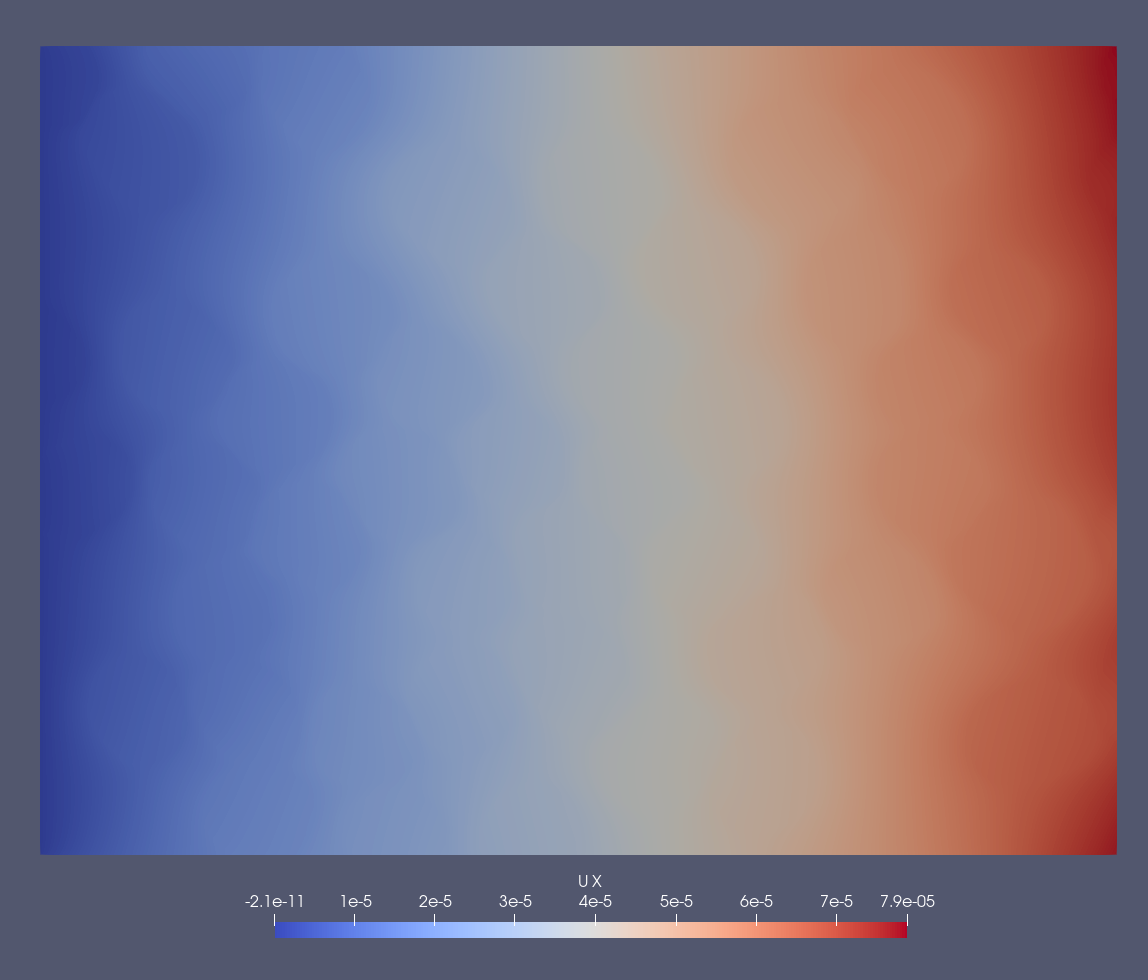
\includegraphics[width=0.7\textwidth]{figures/solution/ux_tracx.png}
    \caption{Résultats de la simulation de traction dans la direction $x$ : champ de déplacement $u_x$.}
    \label{fig:solution_tracx}
\end{figure}

\begin{figure}[H]
    \centering
    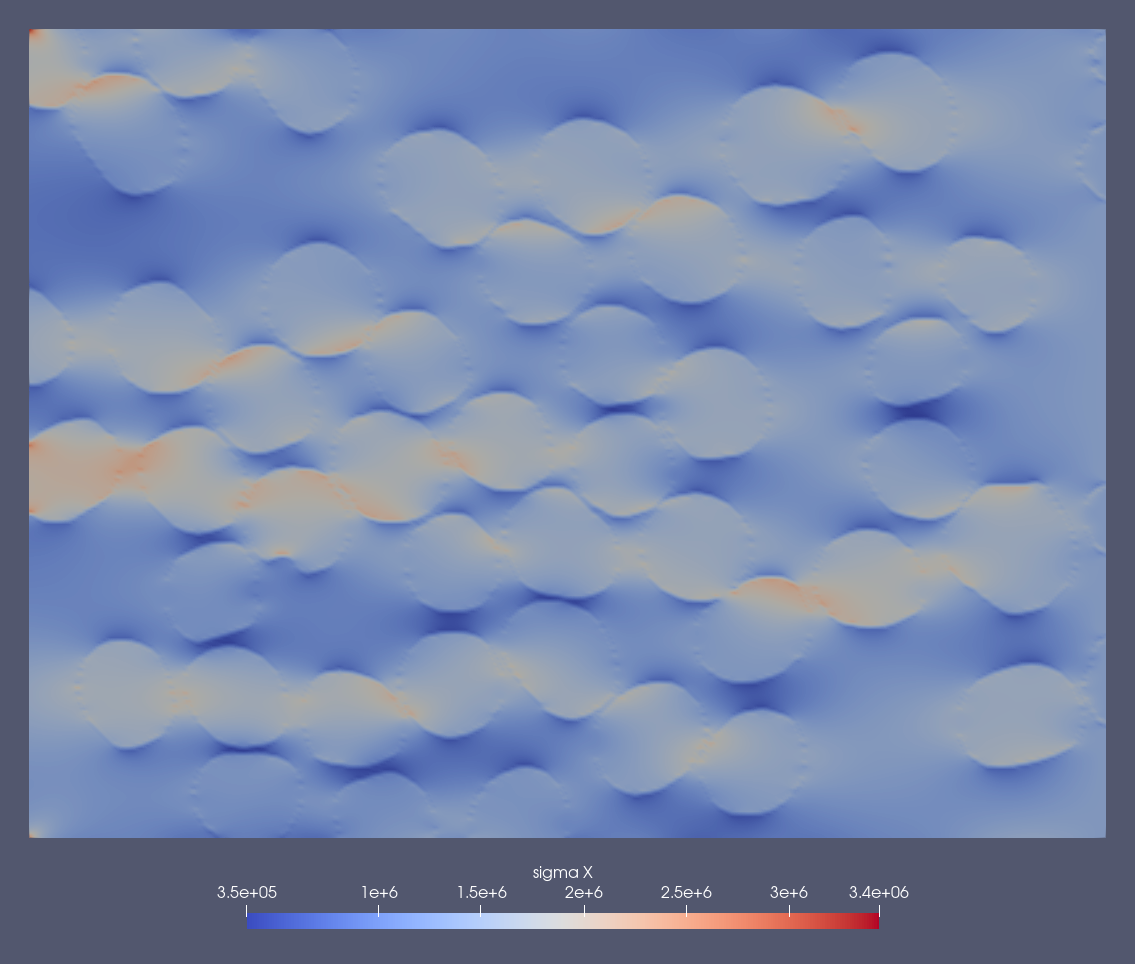
\includegraphics[width=0.49\textwidth]{figures/solution/sigmax_tracx.png}
    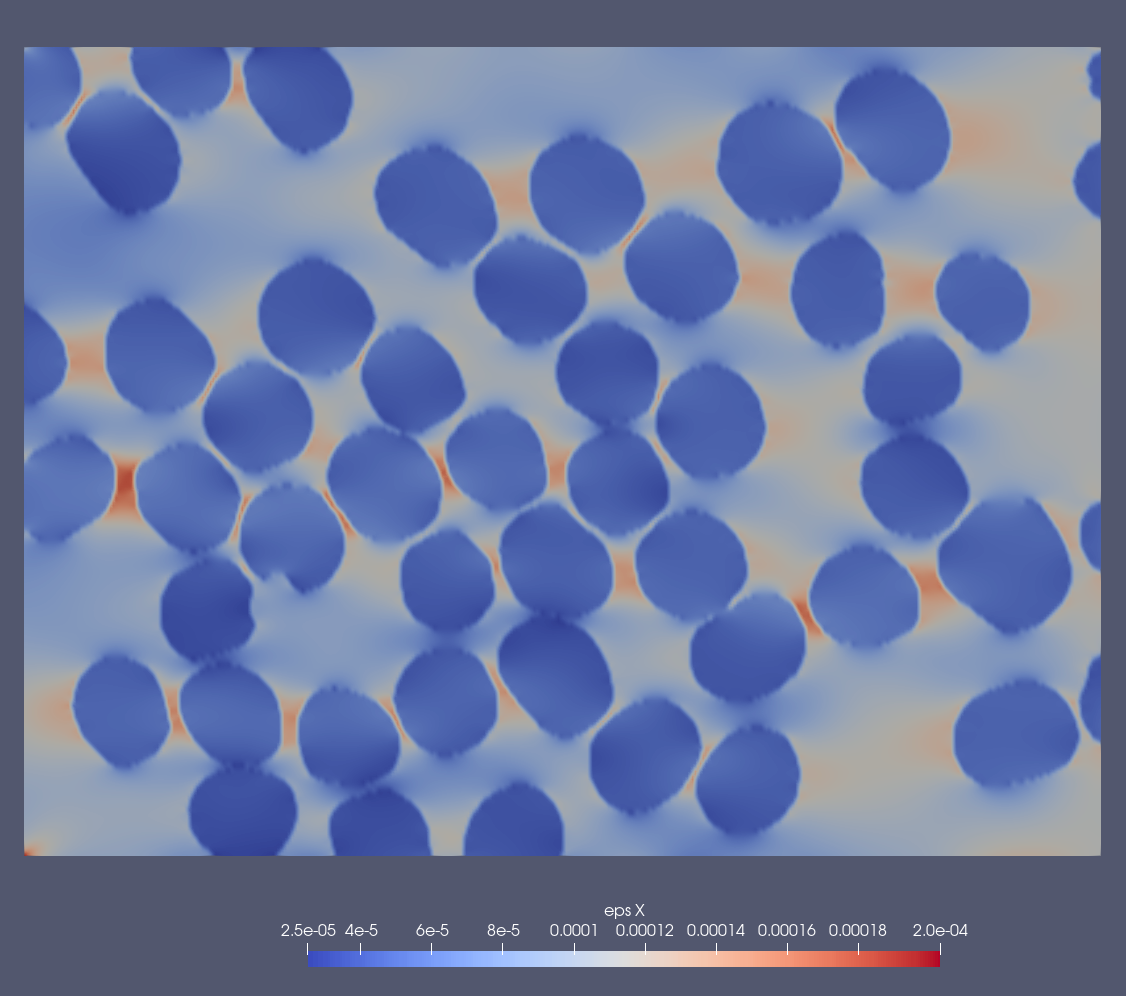
\includegraphics[width=0.49\textwidth]{figures/solution/eps_X_tracx.png}
    \caption{Résultats de la simulation de traction dans la direction $x$ : champ de contrainte $\sigma_{xx}$ (gauche) et champ de déformation $\varepsilon_{xx}$ (droite).}
    \label{fig:solution_tracx_fields}
\end{figure}

Les champs de contrainte et de déformation montrent une hétérogénéité bien plus marquée que sur le déplacement, on distingue clairement les fibres et la matrice, avec les fibres subissant des contraintes et déformations plus fiable que la matrice. Le point le plus intéressant est la zone entre les fibres et la matrice, où l'on observe des gradients de contrainte et de déformation très importants ($\varepsilon_{xx}$ passe de 2.5e-5 dans la fibre à 2.0e-4 à côté dans la matrice). Ces zones de fort gradient sont observées typiquement dans la direction de traction, et sont liées à la forte hétérogénéité du matériau. Elles sont particulièrement présentes lorsque les fibres sont proches les unes des autres, et seraient les zones les plus susceptibles de subir des dommages dans un composite réel, ce qui montre l'intérêt de l'homogénéisation numérique pour identifier ces zones critiques. Parallèlement, des zones de faible contrainte sont observées autour des fibres dans la direction perpendiculaire à la traction (environ 0.35 MPa), soit environ 2 fois plus faible que le chargement appliqué (1e6 N réparti sur une hauteur de 0.75m). Les zones sur-contraintes présentent elles des valeurs d'environ 3 MPa, soit 4 fois plus que le chargement appliqué.

\subsubsection{Traction 2}

Pour l'essai de traction dans la direction $y$, le champ de déplacement $u_y$ et tracé ainsi que la norme du champ de contrainte $\sigma_{\text{mag}} = \sqrt{\sigma_{xx}^2 + \sigma_{yy}^2 + 2\sigma_{xy}^2}$, qui permet d'avoir une vision globale de l'intensité des contraintes dans le domaine, indépendamment de leur orientation.

\begin{figure}[H]
    \centering
    
\includegraphics[width=0.49\textwidth]{figures/solution/uy_tracy.png}
    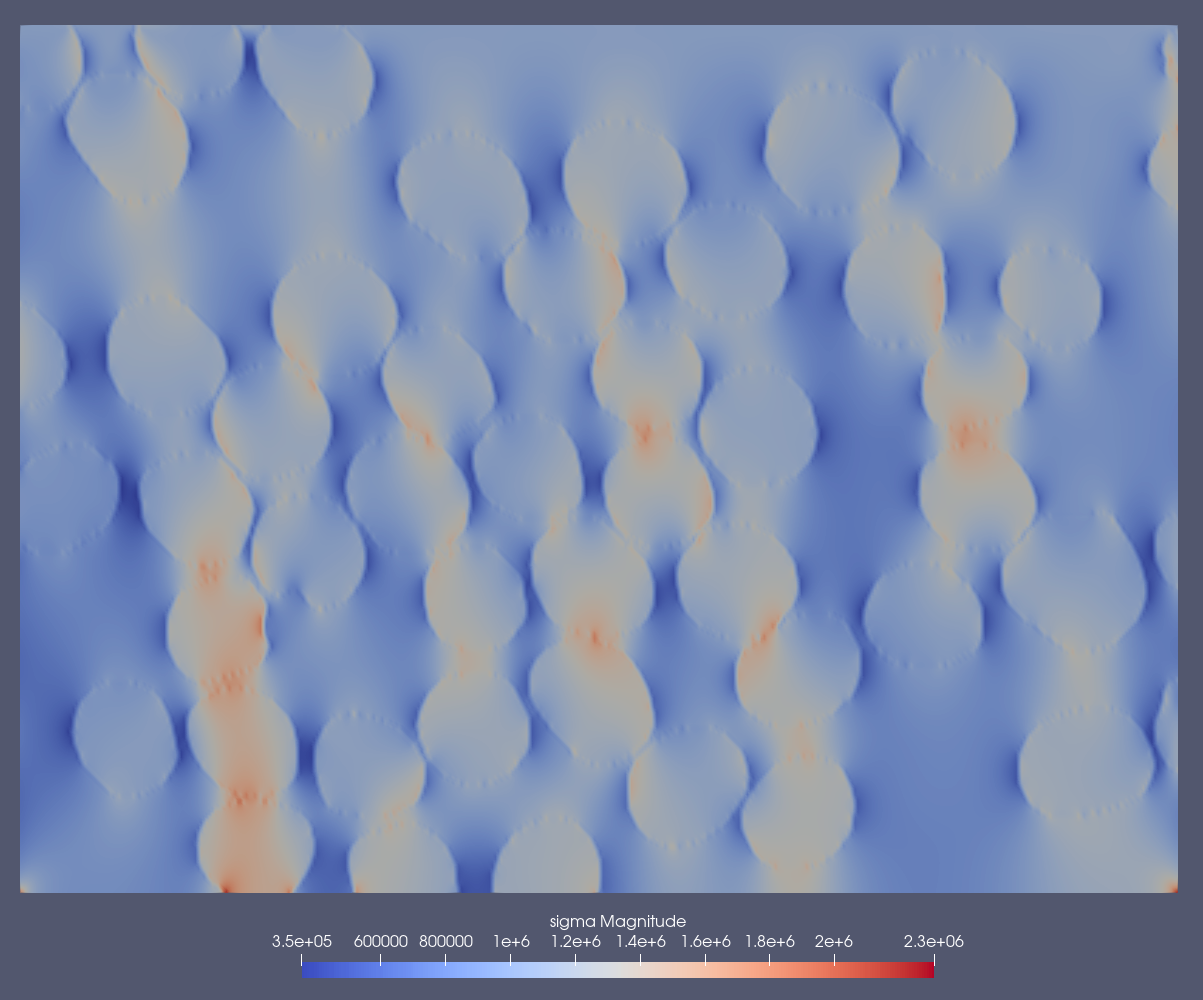
\includegraphics[width=0.49\textwidth]{figures/solution/sigmamag_tracy.png}
    \caption{Résultats de la simulation de traction dans la direction $y$ : champ de déplacement $u_y$ (gauche) et norme du champ de contrainte $\sigma_{\text{mag}}$ (droite).}
    \label{fig:solution_tracy}
\end{figure}

Le comportement des champs est similaire à la traction selon x, avec une rotation du champ de déplacement et de contrainte en fonction de la direction de chargement. Le déplacement est cohérent à la fois avec les conditions aux limites, la nature hétérogène du matériau, ainsi que l'essai de traction selon (coin haut droit moins rigide). La contrainte montre un comportement similaire, avec des gradients de contraintes localisés dans la matrice entre les fibres, principalement dans la direction y dans ce cas. La norme de la contrainte montre des zones présentant des contraintes d'environ 2.3 MPa, soit plus de 2 fois le chargement appliqué (1 MPa), à l'inverse, les zones autour des fibres selon la direction transversale montrent des contraintes d'environ 0.35 MPa. L'interprétation de ces résultats est similaire à la traction selon x, avec des zones de fort gradient de contrainte dans la matrice entre les fibres, qui sont les zones les plus susceptibles de subir des dommages dans un composite réel.

\subsubsection{Cisaillement pur}

Pour illustrer au mieux le cisaillement pur, nous avons choisi de tracer la norme du champ de déformation $\varepsilon_{\text{mag}} = \sqrt{\varepsilon_{xx}^2 + \varepsilon_{yy}^2 + 2\varepsilon_{xy}^2}$, qui permet d'avoir une vision globale de l'intensité des déformations dans le domaine, indépendamment de leur orientation. \\

Le champ montre des zones de forte déformation localisées dans la matrice entre les fibres, avec des valeurs d'environ 0.002, tandis que les fibres présentent des déformations d'environ 4e-4, soit 5 fois plus faibles. Ces zones de forte déformation sont principalement localisées dans la direction de cisaillement, c'est-à-dire orientée à 45° dans le plan. \\

\begin{figure}[H]
    \centering
    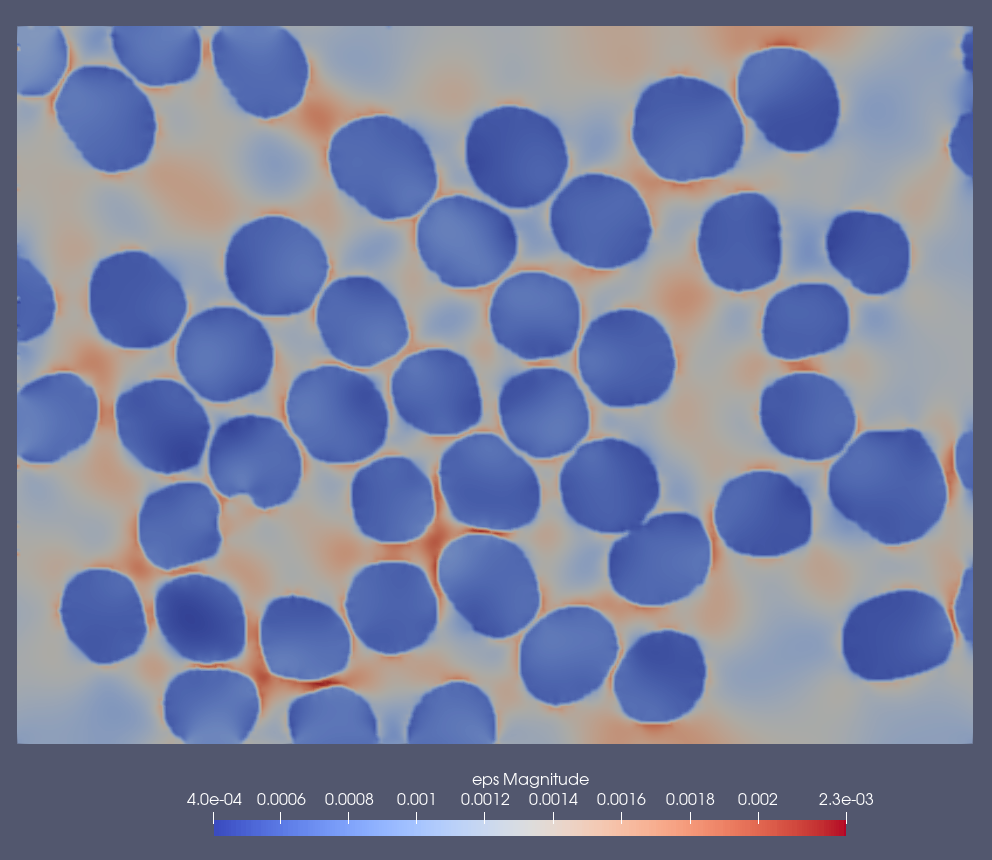
\includegraphics[width=0.60\textwidth]{figures/solution/epsmag_shear.png}
    \caption{Résultats de la simulation de cisaillement pur : norme du champ de déformation $\varepsilon_{\text{mag}}$.}
    \label{fig:solution_shear}
\end{figure} 

Globalement, pour les différents cas, les champs de déplacement, de déformation et de contrainte montrent une cohérence avec les conditions aux limites appliquées, la nature hétérogène du matériau. Les zones de fort gradient de contrainte et de déformation sont principalement localisées dans la matrice entre les fibres, ce qui est cohérent avec la physique du problème, et montre l'intérêt de l'homogénéisation numérique pour identifier ces zones critiques dans un composite réel.

\subsubsection{Propriétés effectives et comparaison aux bornes analytiques} 

Globalement le champ de contrainte est moins hétérogène que le champ de déformation, cela explique l'hypothèse de Reuss qui suppose l'iso-contrainte dans le composite, ce qui n'est pas le cas pour l'hypothèse de Voigt qui suppose l'iso-déformation, ce qui est plus éloigné de la réalité dans le plan transverse d'un composite. Les propriétés effectives pour ce maillage avaient déjà été présentées dans le tableau de convergence en maillage, mais nous les récapitulons ici pour les comparer aux bornes analytiques :
\begin{table}[H]
    \centering
    \begin{tabular}{|l|c|c|c|c|c|}
        \hline
        \textbf{Propriétés} & $E_{11}$ & $E_{22}$ & $G_{12}$ & $\nu_{12}$ & $\nu_{21}$ \\
        \hline
        \textbf{Valeur numérique} & 18,1380 GPa & 18,0515 GPa & 7,1856 GPa & 0,28651 & 0,28522 \\
        \hline
    \end{tabular}
    \caption{Récapitulatif des propriétés effectives du composite.}
    \label{tab:homo_recap}
\end{table}

Premièrement, on observe des valeurs qui sont cohérentes physiquement, avec les modules d'Young compris entre ceux de la matrice (12 GPa) et la fibre (34 GPa), de même pour le coefficient de Poisson. Les modules $E_{11}$ et $E_{22}$ sont presque égaux (environ 18.1 GPa), de même pour les coefficients de Poisson $\nu_{12}$ et $\nu_{21}$ (environ 0.286). Cela est cohérent avec l'hypothèse qui stipule que le composite se comporte de manière isotrope dans le plan transverse. Un bon paramètre pour vérifier la robustesse du solveur est la symétrie du tenseur de souplesse/rigidité, qui doit impérativement être assurée :

\begin{align}
    S_{12} &= \frac{\nu_{12}}{E_{11}} = -1.5796e-11 ,\\
    S_{21} &= \frac{\nu_{21}}{E_{22}} = -1.58004e-11
\end{align}

Il y a un écart relatif très faible entre ces valeurs d'environ 0.03\%, ce qui valide le schéma éléments finis pour un maillage composite. Pour la suite de l'étude, on notera les propriétés numériques obtenues à partir de l'homogénéisation numérique par les notations suivantes, qui correspondent à des propriétés effectives isotropes dans le plan transverse :

\begin{itemize}
    \item $E_T$ : Module d'Young transversal (moyenne de $E_{11} \approx E_{22}$)
    \item $G_{LT}$ : Module de cisaillement dans le plan transverse (égal à $G_{12}$)
    \item $\nu_{TT}$ : Coefficient de Poisson dans le plan transverse (moyenne de $\nu_{12} \approx \nu_{21}$)
\end{itemize}

\vspace{0.2cm}
 Il est désormais intéressant de comparer ces propriétés effectives numériques aux bornes analytiques de Voigt, Reuss, Hill et Halpin-Tsai, qui sont des modèles classiques d'homogénéisation pour les composites. Pour cela, nous extrayons la fraction volumique de fibre du maillage, qui vaut 0.449, et nous calculons les propriétés effectives correspondantes à partir des formules analytiques de ces modèles, présentés dans la partie théorique :
\begin{table}[H]
    \centering
    \begin{tabular}{|l|c|c|c|c|c|}
        \hline
        & \textbf{Numérique} & \textbf{Voigt} & \textbf{Reuss} & \textbf{Hill} & \textbf{Halpin-Tsai ($\xi = 0.8$)} \\
        \hline
        $E_T$ (GPa) & 18,095 & 21,898 & 16,928 & 19,413 & 18,344 \\
        $G_{LT}$ (GPa) & 7,1856 & 8,6576 & 6,5674 & 7,6125 & 7,1499 \\
        $\nu_{TT}$ & 0,28587 & 0,27750 & 0,27523 & 0,27637 & 0,27630 \\
        \hline
    \end{tabular}
    \caption{Comparaison des propriétés effectives numériques avec les bornes analytiques de Voigt, Reuss, Hill et Halpin-Tsai.}
    \label{tab:homo_bounds}
\end{table}

Les bornes analytiques classiques comme Voigt et Reuss ne donnent pas des résultats satisfaisants : 21\% d'écart relatif pour Voigt par rapport à la valeur numérique, et 6.45\% pour Reuss. La borne de Reuss est cependant plus précise, car elle fait l'hypothèse d'une contrainte uniforme, ce qui est plus le cas dans le plan transverse que dans le plan longitudinal. La moyenne de Hill donne des résultats similaires (7.3\% d'écart sur $E_T$) car elle ne prend pas en compte la nature du VER. Cependant, le modèle d'Halpin-Tsai ajusté avec un bon paramètre ($\xi = 0.8$) donne des résultats bien plus proches des valeurs numériques, avec seulement 1.3\% d'écart sur $E_T$ et 0.5\% sur $G_{LT}$. Il serait possible d'ajuster le paramètre $\xi$ différemment pour E et G afin d'avoir un modèle très précis. \\

Dans la littérature, on retrouve souvent des valeurs de $\xi = 2$ pour le plan transverse au fibre, le fait d'avoir une valeur plus faible pour mieux capter les résultats est sûrement liée avec la nature désorganisée du VER, comme l'a montré les différentes images de la partie U-Net. En effet, on a des zones de porosités (maillées comme de la matrice ici), et des zones de fibres plus ou moins denses, pas un réseau parfaitement hexagonal. Concernant le coefficient de Poisson, aucun modèle analytique ne se démarque vraiment, avec des écarts relatifs d'environ 3\%, ce qui peut soit être lié à une erreur numérique, soit à l'imprécision des modèles analytiques pour ce type de composite. \\

Il est difficile de savoir si ce sont les bornes analytiques, ou bien les résultats EF qui sont les plus fiables pour notre composite, mais il est intéressant de voir que les résultats numériques sont plus proches du modèle d'Halpin-Tsai, qui prend en compte la nature du VER, que des modèles classiques de Voigt et Reuss. Cela montre l'intérêt de l'homogénéisation numérique pour obtenir des propriétés effectives plus précises, qui peuvent ensuite être utilisées pour ajuster des modèles analytiques plus simples, comme celui d'Halpin-Tsai.


\subsection{Étude de l'influence de la fraction volumique de fibre}

Pour le moment, l'ensemble de l'étude a été réalisée pour un VER avec une fraction volumique de fibre d'environ 0.45, qui est relativement réaliste pour un composite C/C. Cependant, il est intéressant d'étudier l'influence de la fraction volumique de fibre sur les propriétés effectives du composite, en générant différents maillages à partir de la segmentation U-Net, avec des fractions volumiques allant de 0.25 à 0.57. Pour cela, nous avons utilisé les différentes images issues de la segmentation U-Net, qui présentent des fractions volumiques différentes, et nous avons appliqué la même démarche d'homogénéisation numérique pour extraire les propriétés effectives correspondantes à chaque fraction volumique. Cela permet réellement d'étudier l'influence de la fraction volumique de fibre sur les propriétés effectives du composite, et de comparer les résultats numériques aux modèles analytiques qui prédisent l'évolution des propriétés en fonction de la fraction volumique. \\

\begin{table}[H]
    \centering
    \footnotesize
    \begin{tabular}{|l|c|c|c|c|c|c|c|c|c|}
        \hline
        \textbf{Propriété} $\backslash$ \textbf{$V_f$} 
        & \textbf{0,252} & \textbf{0,277} & \textbf{0,364} & \textbf{0,375} 
        & \textbf{0,395} & \textbf{0,419} & \textbf{0,450} & \textbf{0,500} & \textbf{0,572} \\
        \hline
        $E_T$ (GPa) & 15,01216 & 15,3633 & 16,6740 & 16,8533 & 17,2560 & 17,60769 & 18,09548 & 18,9362 & 20,5871 \\
        \hline
        $G_{LT}$ (GPa) & 5,8392 & 5,9829 & 6,5525 & 6,6464 & 6,7804 & 6,9281 & 7,1855 & 7,6028 & 8,1732 \\
        \hline
        $\nu_{TT}$ & 0,2921 & 0,2897 & 0,2876 & 0,2876 & 0,2851 & 0,2842 & 0,2859 & 0,2830 & 0,2756 \\
        \hline
    \end{tabular}
    \caption{Évolution des propriétés effectives moyennes en fonction de la fraction volumique de fibres $V_f$.}
    \label{tab:etude_vf}
\end{table}

Les données sont alors exportées dans des fichiers CSV, et un script de post-traitement en Python est utilisé pour tracer l'évolution des propriétés effectives $E_T$, $G_{LT}$ et $\nu_{TT}$ en fonction de la fraction volumique de fibre, et les comparer aux bornes analytiques de Voigt, Reuss, Hill et Halpin-Tsai. Le paramètre $\xi$ pour le modèle d'Halpin-Tsai est ajusté à 0.6 pour mieux capter l'évolution de $E_T$ en fonction de la fraction volumique, et à 0.8 pour $G_{LT}$. 
\begin{figure}[H]
    \centering
    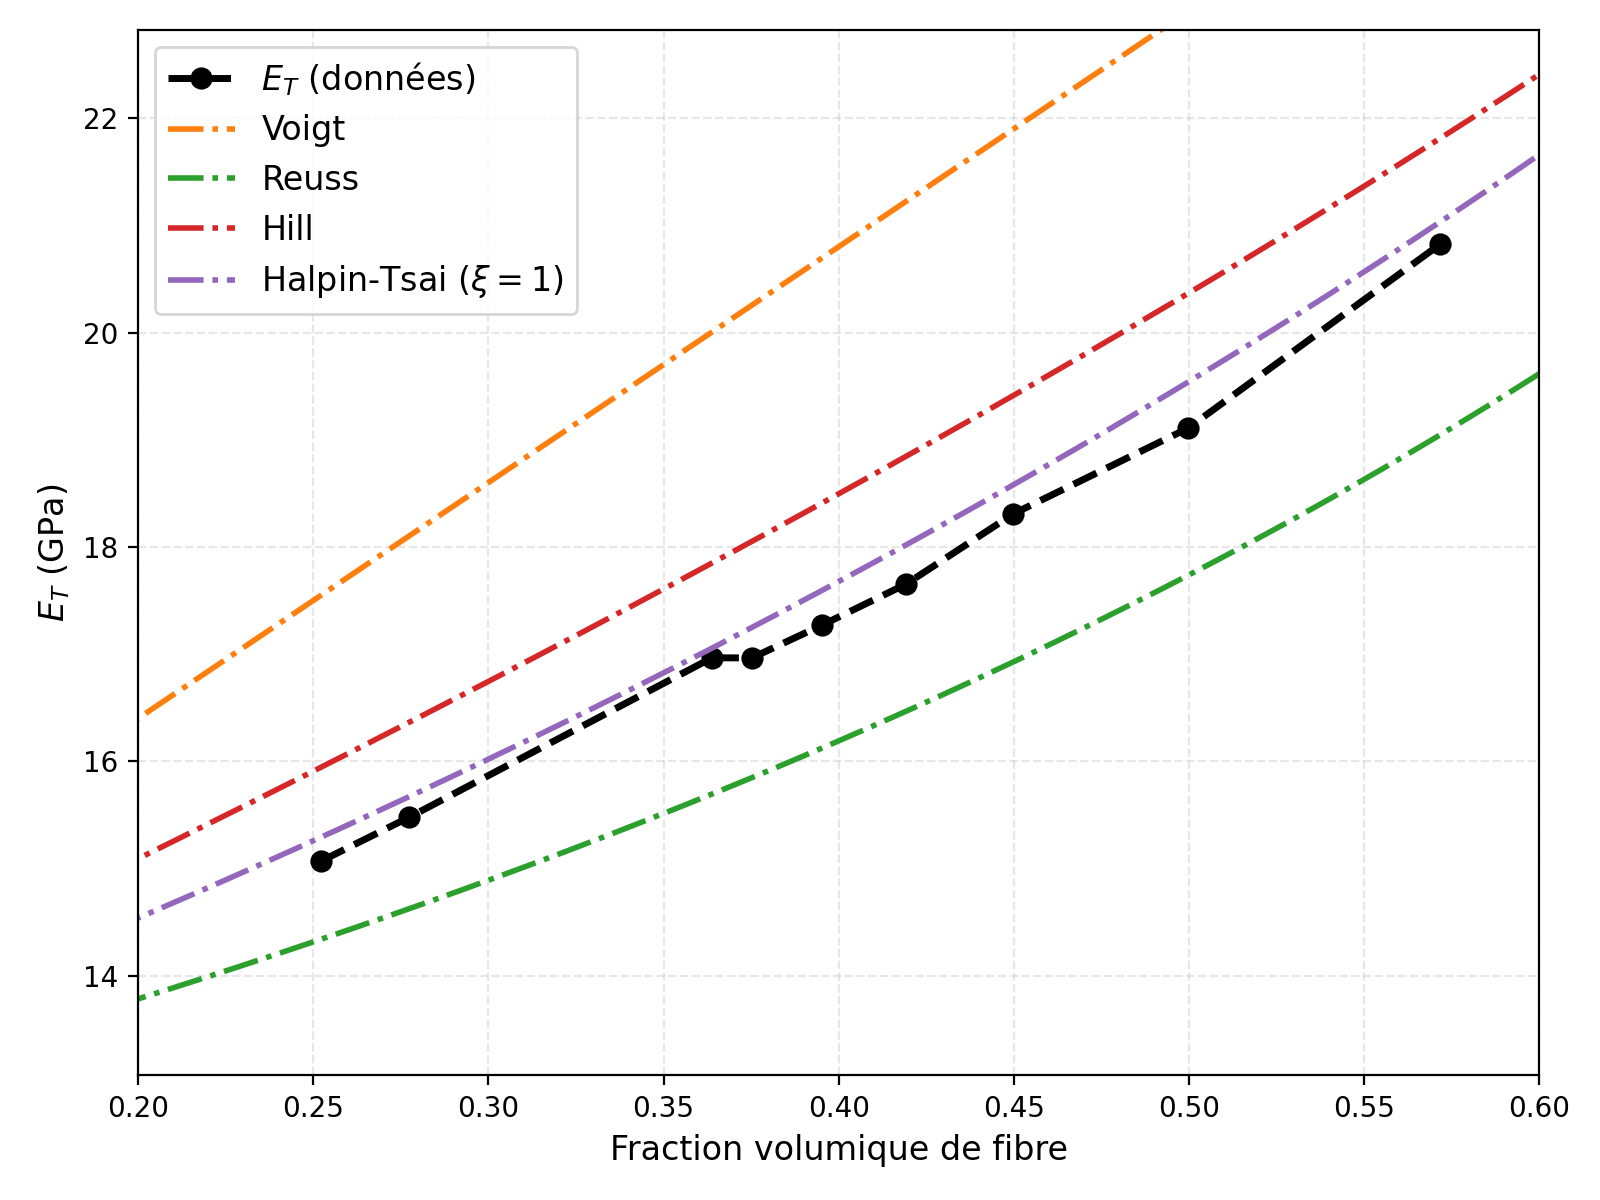
\includegraphics[width=0.49\textwidth]{figures/etude_vf_E.png}
    
\includegraphics[width=0.49\textwidth]{figures/etude_vf_G.png}
    \caption{Évolution du module d'Young transversal $E_T$ (gauche) et du module de cisaillement $G_{LT}$ (droite) en fonction de la fraction volumique de fibre $V_f$. Chaque point représentant une valeur numérique obtenue à partir d'un maillage généré via U-Net à partir de la base d'images. Les bornes de Voigt, Reuss, Hill et Halpin-Tsai sont tracées pour référence en couleurs.}
    \label{fig:etude_vf_E}
\end{figure}

Les propriétés effectives montrent une évolution cohérente avec la physique du problème, avec une augmentation du module d'Young et du module de cisaillement à mesure que la fraction volumique de fibre augmente, ce qui est attendu car les fibres sont plus rigides que la matrice. La borne de Voigt surestime les propriétés effectives, tandis que la borne de Reuss les sous-estime, la moyenne de Hill donne des résultats entre les deux mais ne capte pas vraiment l'évolution. Cependant, le modèle d'Halpin-Tsai, ajusté avec des paramètres $\xi$ adaptés, donne une très bonne approximation de l'évolution des propriétés effectives en fonction de la fraction volumique, ce qui montre l'intérêt de ce modèle pour capturer la nature du VER. Le tableau ci-dessous résume l'erreur moyenne absolue (MAE) pour chaque modèle analytique par rapport aux résultats numériques pour $E_T$ et $G_{LT}$.
\begin{table}[H]
    \centering
    \begin{tabular}{|l|c|c|}
    \hline
    \textbf{Modèle} & \textbf{MAE $E_T$} & \textbf{MAE $G_{LT}$} \\
    \hline
    Voigt        & 0.1644 & 0.1652 \\
    Reuss        & 0.0644 & 0.0828 \\
    Hill         & 0.0638 & 0.0573 \\
    Halpin-Tsai  & 0.0034 & 0.0041 \\
    \hline
    \end{tabular}
    \caption{Comparaison des erreurs absolues moyennes (MAE) pour $E_T$ et $G_{LT}$.}
\end{table}

Les valeurs illustrent clairement la supériorité du modèle d'Halpin-Tsai pour capturer l'évolution des propriétés effectives en fonction de la fraction volumique de fibre, des erreurs très faibles de l'ordre de 0.0034GPa et 0.0041GPa pour $E_T$ et $G_{LT}$ respectivement, tandis que les autres modèles présentent des erreurs beaucoup plus importantes, notamment Voigt qui surestime fortement les propriétés effectives. L'évolution de $\nu_{TT}$ en fonction de la fraction volumique est plus complexe, avec une légère tendance à la baisse à mesure que la fraction volumique augmente, mais toujours un décalage important avec les modèles analytiques qui sous-estiment la valeur de ce coefficient. \\

Globalement, cette étude montre que la fraction volumique de fibre a un impact significatif sur les propriétés effectives du composite, et qu'un modèle analytique ajusté comme celui d'Halpin-Tsai peut capturer de manière très précise cette évolution, ce qui est très utile pour la conception de composites avec des propriétés mécaniques spécifiques.

\subsection{Étude de l'influence des porosités}

\subsubsection{Contexte et modélisation des porosités}
Les porosités sont des défauts de fabrication courants dans les composites C/C, résultant de l'infiltration incomplète de la matrice ou de la libération de gaz lors du traitement thermique. Elles peuvent être modélisées comme des inclusions de matériau très faible rigidité (ou même des trous) dans le maillage, ce qui permet d'étudier leur impact sur les propriétés mécaniques effectives du composite. La segmentation U-Net ainsi que la modularité du code en C++ permettent d'intégrer facilement les porosités dans le maillage et de les traiter comme un troisième matériau supposé isotrope. D'un point de vue numérique, il est préférable de traiter ces porosités comme des matériaux avec des propriétés négligeables, mais suffisamment grandes pour éviter des problèmes de convergence :
\begin{itemize}
    \item Module de Young : $E_p = 0{,}01$ GPa
    \item Coefficient de Poisson : $\nu_p = 0{,}3$
\end{itemize}

Le module d'élasticité (1000 fois plus faible que la matrice) permet de simuler le vide de manière réaliste, tout en assurant la stabilité du schéma EF. Le coefficient de poisson est fixé arbitrairement à une valeur standard (peu d'influence). La simulation est exactement la même que pour le cas sans porosités (pas de CL supplémentaires), mais nous choisissons un VER intéressant à mailler qui présente une porosité centrale de taille significative, ainsi que d'autres porosités réparties dans le VER :
\begin{figure}[H]
    \centering
    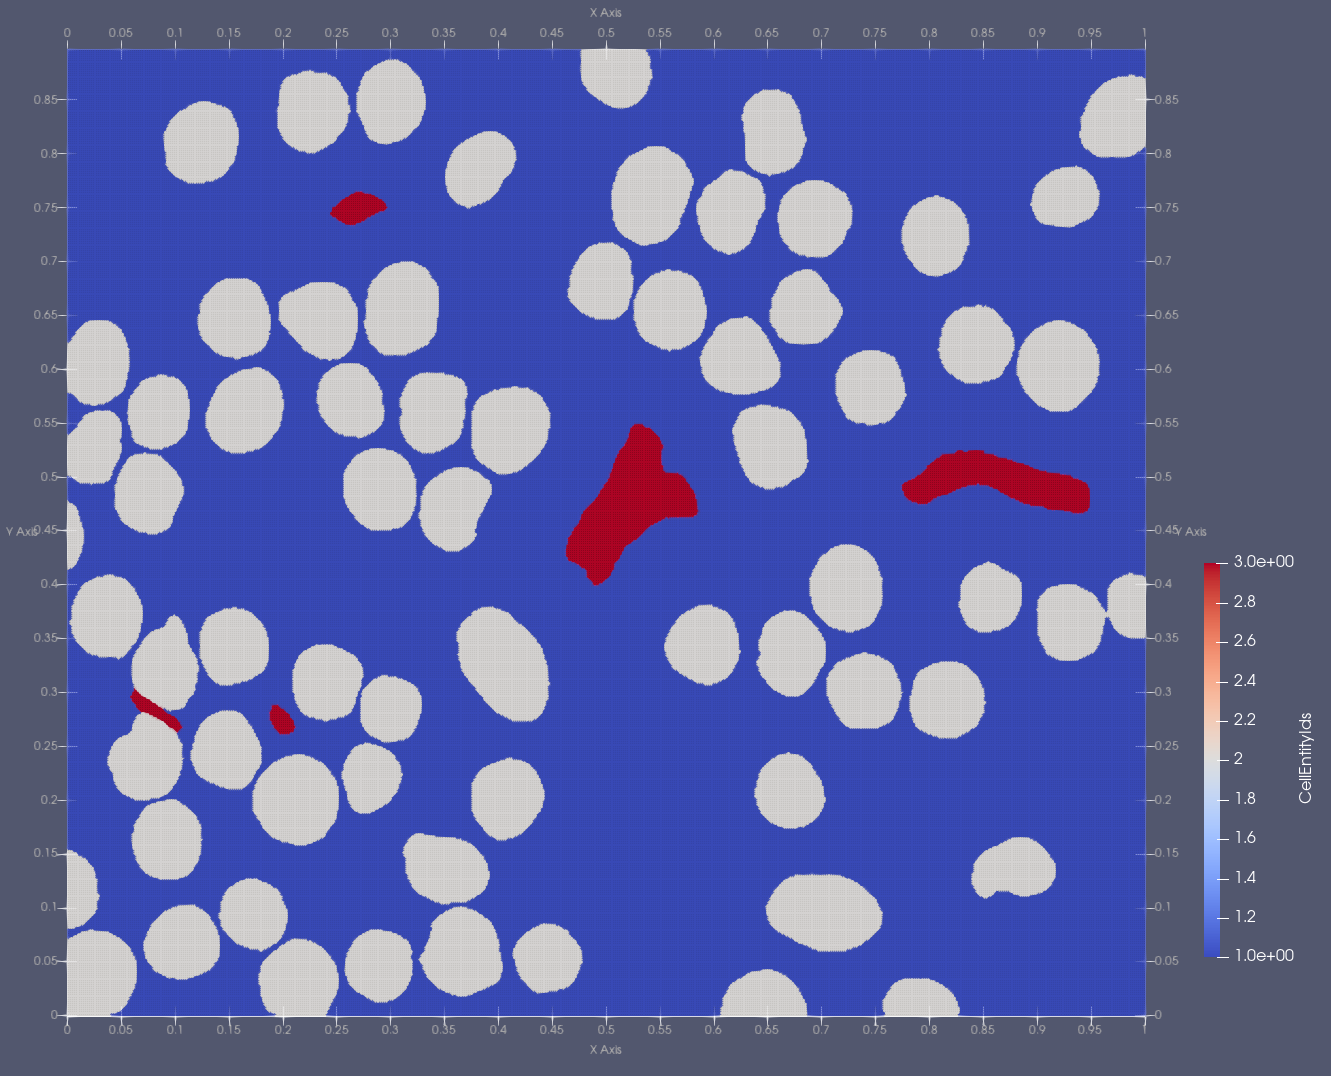
\includegraphics[width=0.65\textwidth]{figures/pores/mesh.png}
    \caption{Maillage utilisé pour les simulations de porosité, généré par U-Net. Matrice (bleu), Fibre (gris), Porosité (rouge).}
    \label{fig:mesh_pores}
\end{figure}

La taille de maille (downscale fixé à 3) est fixée à $0.0018$, avec 292352 éléments, encore plus précis que les simulations précédentes, pour garantir une bonne résolution de la concentration de contraintes.

\subsubsection{Résultats et analyse}

Les propriétés effectives sont extraites avec les porosités, et comparées aux résultats en considérant les porosités comme matrice (comme précédemment), afin d'évaluer l'impact de ces défauts sur les propriétés mécaniques du composite. Le tableau ci-dessous résume les propriétés effectives avec et sans porosités, ainsi que les propriétés du maillage et la fraction volumique de fibres.

\begin{table}[H]
    \centering
    \begin{tabular}{|l|c|c|c|c|c|}
        \hline
        \textbf{Propriétés} & $E_{11}$ & $E_{22}$ & $G_{12}$ & $\nu_{12}$ & $\nu_{21}$\\
        \hline
        \textbf{Avec porosités} & 14,591 GPa & 13,655 GPa & 5,5964 GPa & 0,2883 & 0,2706 \\ 
        \hline
        \textbf{Sans porosités} & 15,618 GPa & 15,541 GPa & 6,0735 GPa & 0,2892 & 0,2880 \\ 
        \hline
    \end{tabular}
    \caption{Récapitulatif des propriétés effectives du composite.}
    \label{tab:porosites_prop}
\end{table}

Les propriétés effectives montrent une diminution significative du module d'Young et du module de cisaillement, avec une réduction d'environ 7\% pour $E_{11}$, 10\% pour $E_{22}$ et 8\% pour $G_{12}$, ce qui illustre l'impact négatif des porosités sur les propriétés mécaniques du composite. Le matériau était isotrope dans le plan transverse sans porosités, mais avec, on observe une anisotropie plus marquée, avec $E_{11}$ plus élevé que $E_{22}$, ce qui est dû aux formes et positions des porosités qui ne sont pas symétriques. Cette anisotropie n'est pas numérique, car si l'on compare la symétrie du tenseur de souplesse avec porosités, on a :
\begin{align}
    S_{12} &= \frac{\nu{12}}{E_{11}} = 1.9756e-11, \\
    S_{21} &= \frac{\nu{21}}{E_{22}} = 1.9816e-11,
\end{align}

Soit un écart de seulement 0.3\%, ce qui est très faible, et montre que le solveur est robuste même en présence de porosités. Analysons maintenant les champs de déplacement et de contrainte pour la simulation de traction dans la direction $x$ avec porosités, afin d'illustrer l'impact de ces défauts sur les champs mécaniques.

\begin{figure}[H]
    \centering
    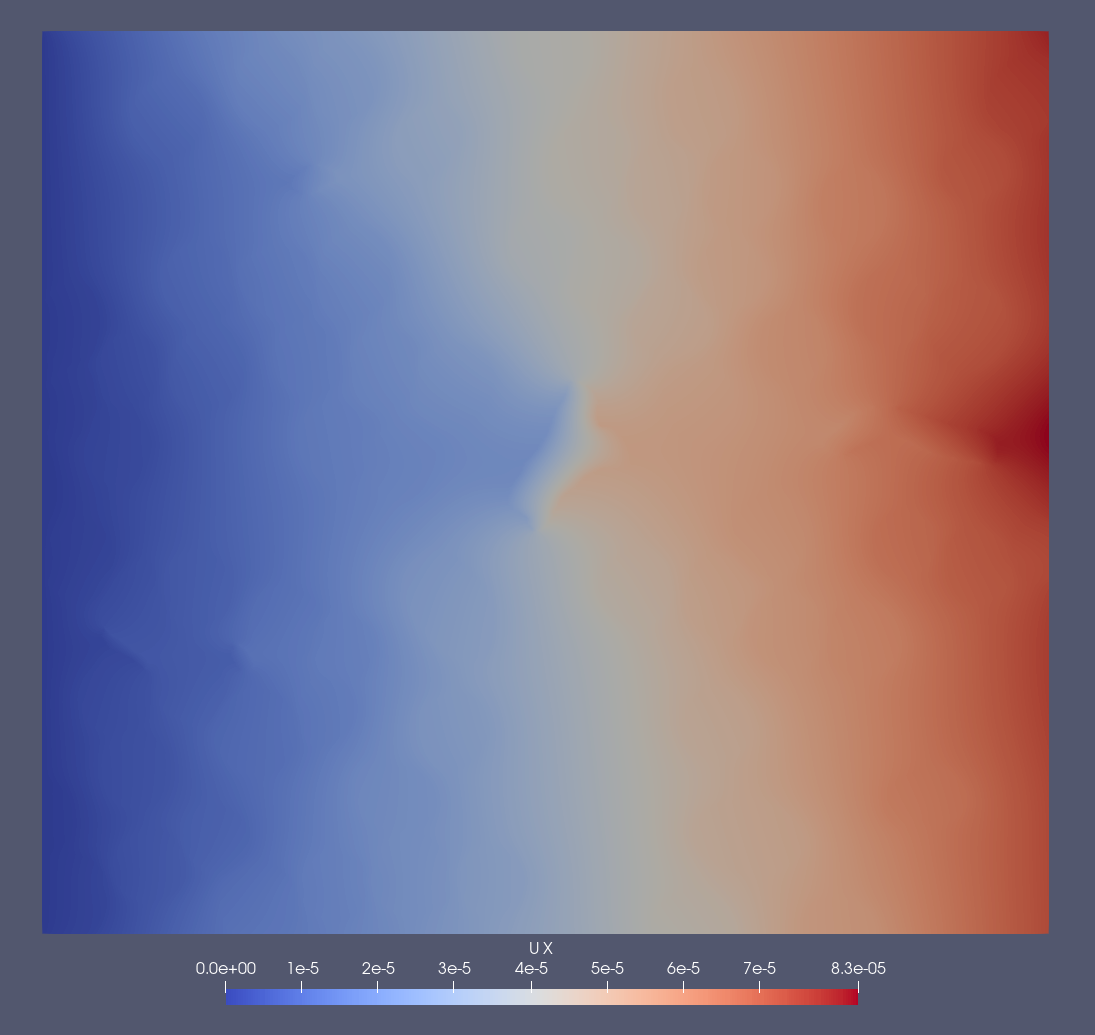
\includegraphics[width=0.49\textwidth]{figures/pores/ux.png}
    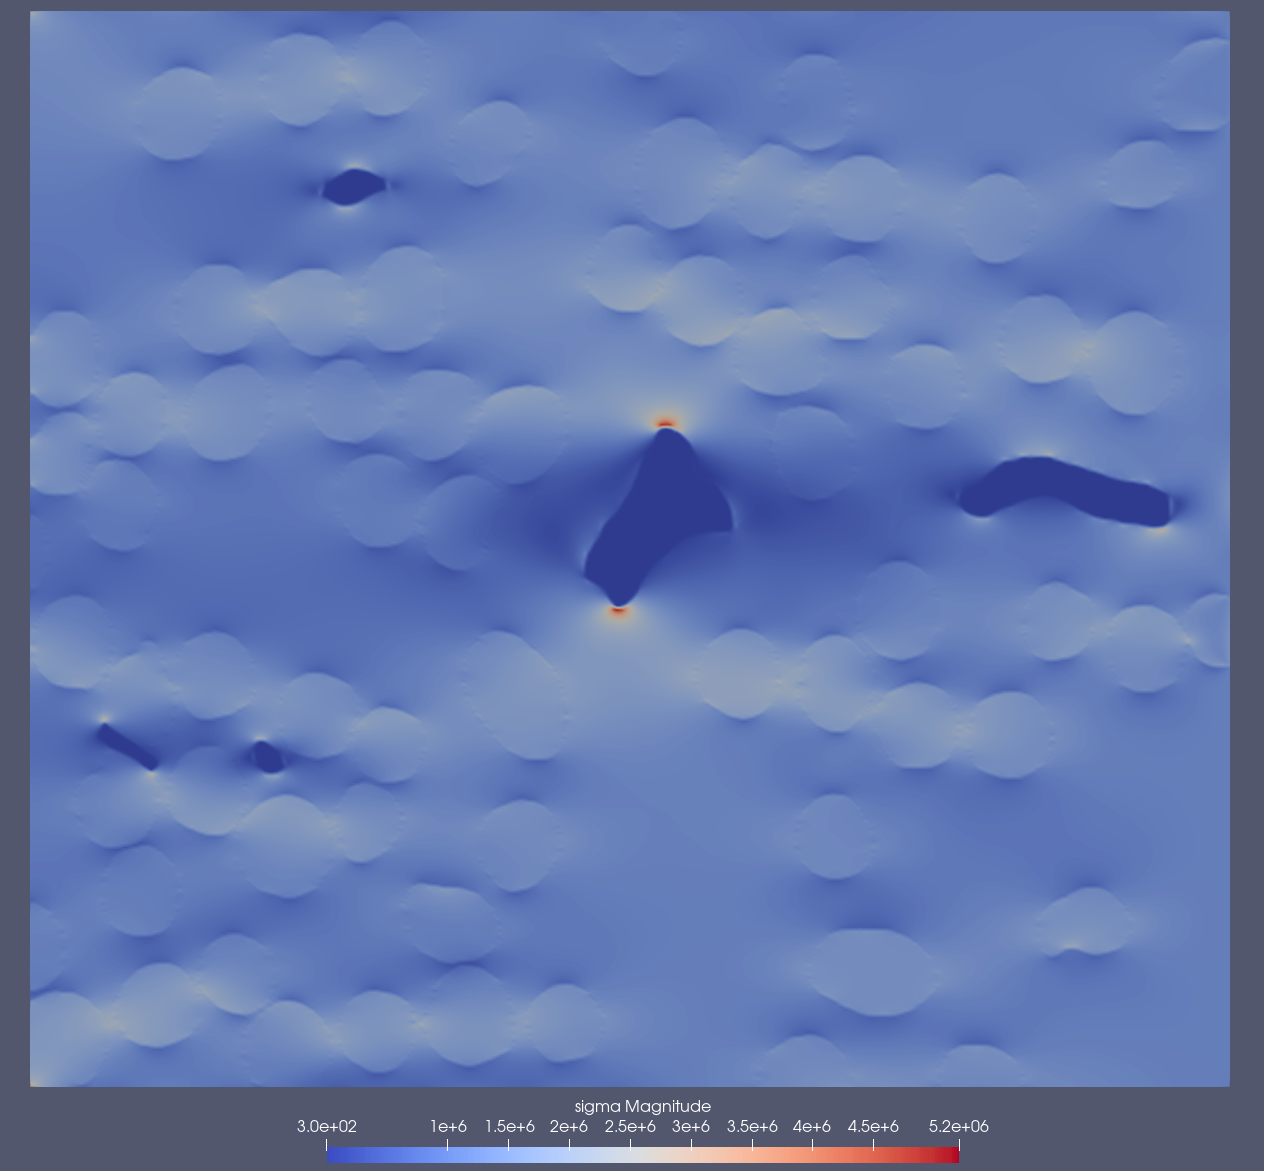
\includegraphics[width=0.49\textwidth]{figures/pores/sigmamag.png}
    \caption{Champs de déplacement $u_x$ (gauche) et norme du champ de contrainte $\sigma_{\text{mag}}$ (droite) pour une simulation de traction dans la direction $x$ avec porosités.}
    \label{fig:pores_fields}
\end{figure}

Sur le champ de déplacement à gauche, une forte hétérogénéité est observée, avec une zone de "fracture" autour de la porosité centrale, avec un fort gradient de part et d'autre. Une autre porosité plus à droite du domaine montre un déplacement très important, ce qui est cohérent avec la nature des défauts et le chargement imposé. La norme du champ de contrainte sur la figure droite montre des zones de forte concentration de contraintes autour des porosités, avec des valeurs allant jusqu'à 5.2 MPa, soit plus de 5 fois le chargement appliqué. Ces zones sont situées autour des porosités, perpendiculairement à la direction de traction. \\

Il est possible de faire une analogie avec la solution de Kirsch pour une inclusion circulaire dans un matériau infini. Sous ces conditions, la solution de Kirsch prédit une concentration de contraintes maximale d'environ 3 fois le chargement appliqué, et une contrainte minimale égale à l'opposé du chargement appliqué, situé dans l'axe de la direction de traction. Nous présentons ci-dessous les champs de contrainte $\sigma_{xx}$ et $\sigma_{yy}$ sur la partie zoomée autour de la porosité centrale:
\begin{figure}[H]
    \centering
    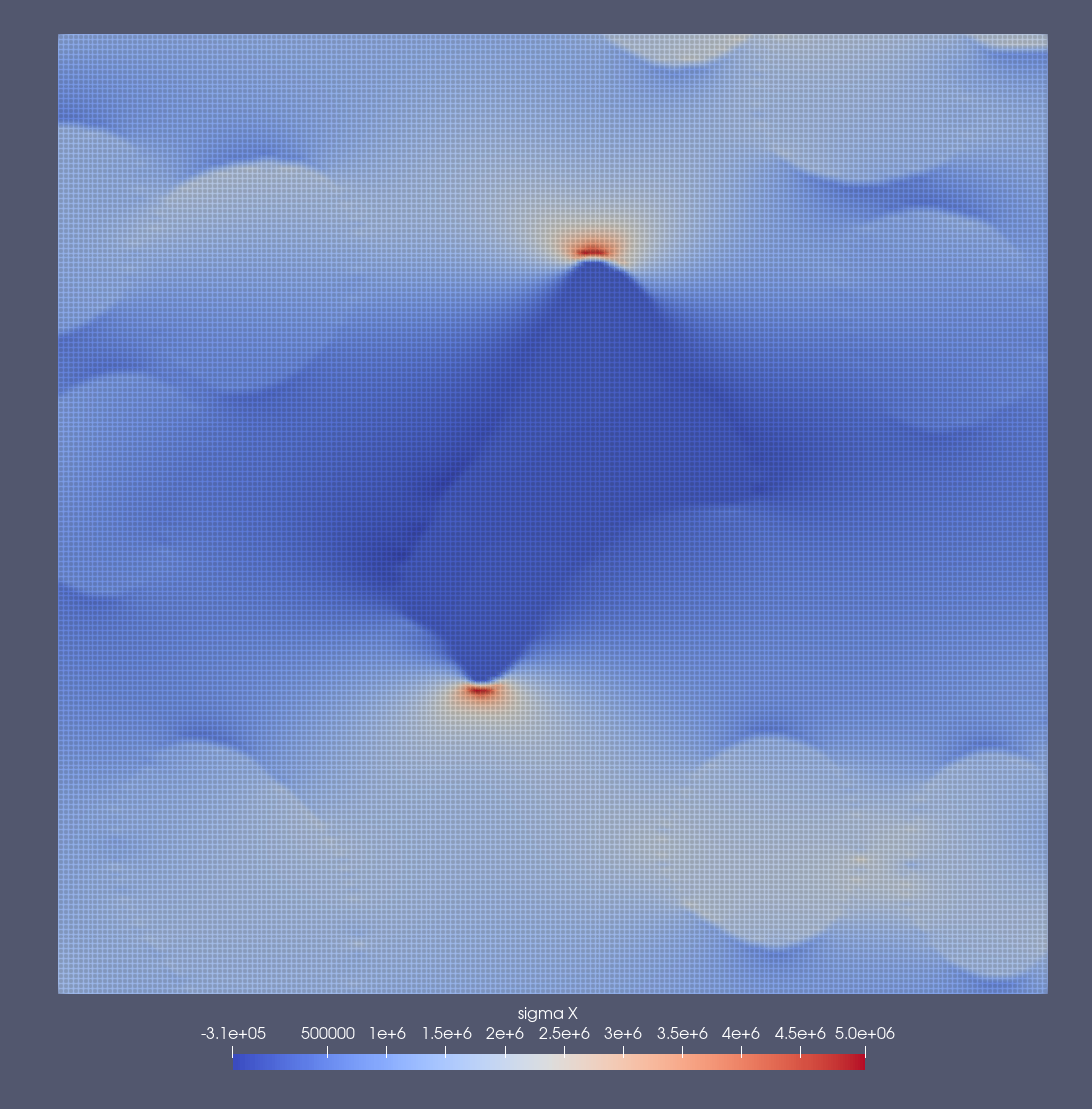
\includegraphics[width=0.49\textwidth]{figures/pores/sigmax.png}
    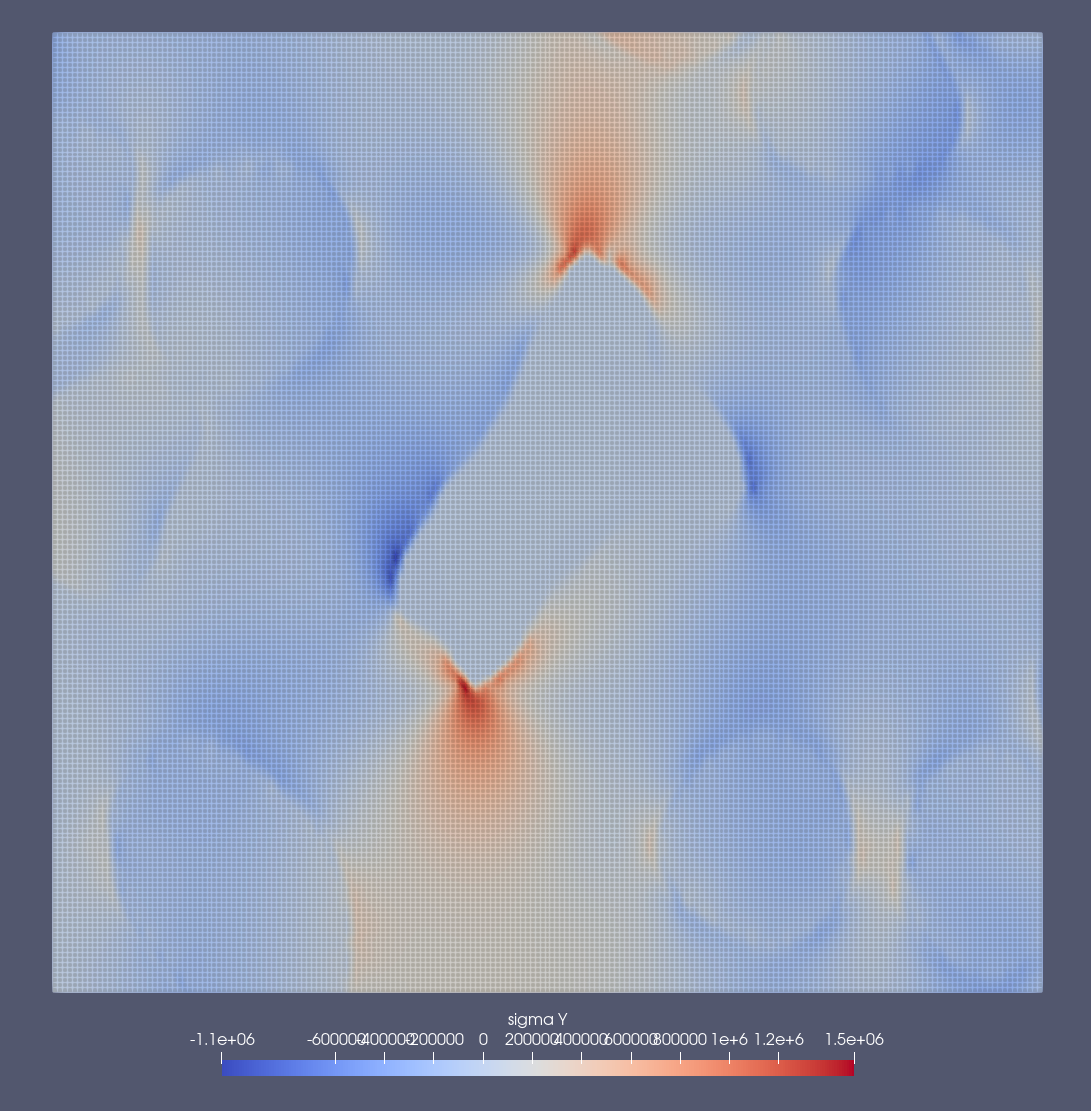
\includegraphics[width=0.49\textwidth]{figures/pores/sigmay.png}
    \caption{Champs de contrainte $\sigma_{xx}$ (gauche) et $\sigma_{yy}$ (droite) dans une zone zoomée autour de la porosité centrale. Le maillage est aussi illustré pour montrer la résolution autour de la porosité.}
    \label{fig:pores_sigmax_sigmay}
\end{figure}

Comme prévu, les contraintes maximales à environ 5 MPa (pour $\sigma_{xx}$) sont situées perpendiculairement à la direction de traction, pour des angles de 90° et 270° par rapport à la direction de traction, tandis que les contraintes minimales d'environ -1.1 MPa (pour $\sigma_{yy}$) sont situées dans l'axe de la direction de traction, à 0° et 180°. Les ordres de grandeurs sont cohérents avec la solution proposée par Kirsch, bien que dans notre cas, la porosité n'est pas un trou parfait, ni circulaire, ni dans un matériau infini, ce qui explique les écarts observés. Cependant, la tendance générale est respectée, avec des zones de forte concentration de contraintes autour des porosités, ce qui montre que le code éléments finis est capable de capturer correctement l'impact des défauts sur les champs mécaniques. \\

Nous présentons ci-dessous les champs de déplacement $u_y$ et de norme de contrainte $\sigma_{\text{mag}}$ pour la simulation de traction dans la direction $y$, afin d'illustrer l'impact des porosités sur les champs mécaniques dans une autre direction de chargement.

\begin{figure}[H]
    \centering
    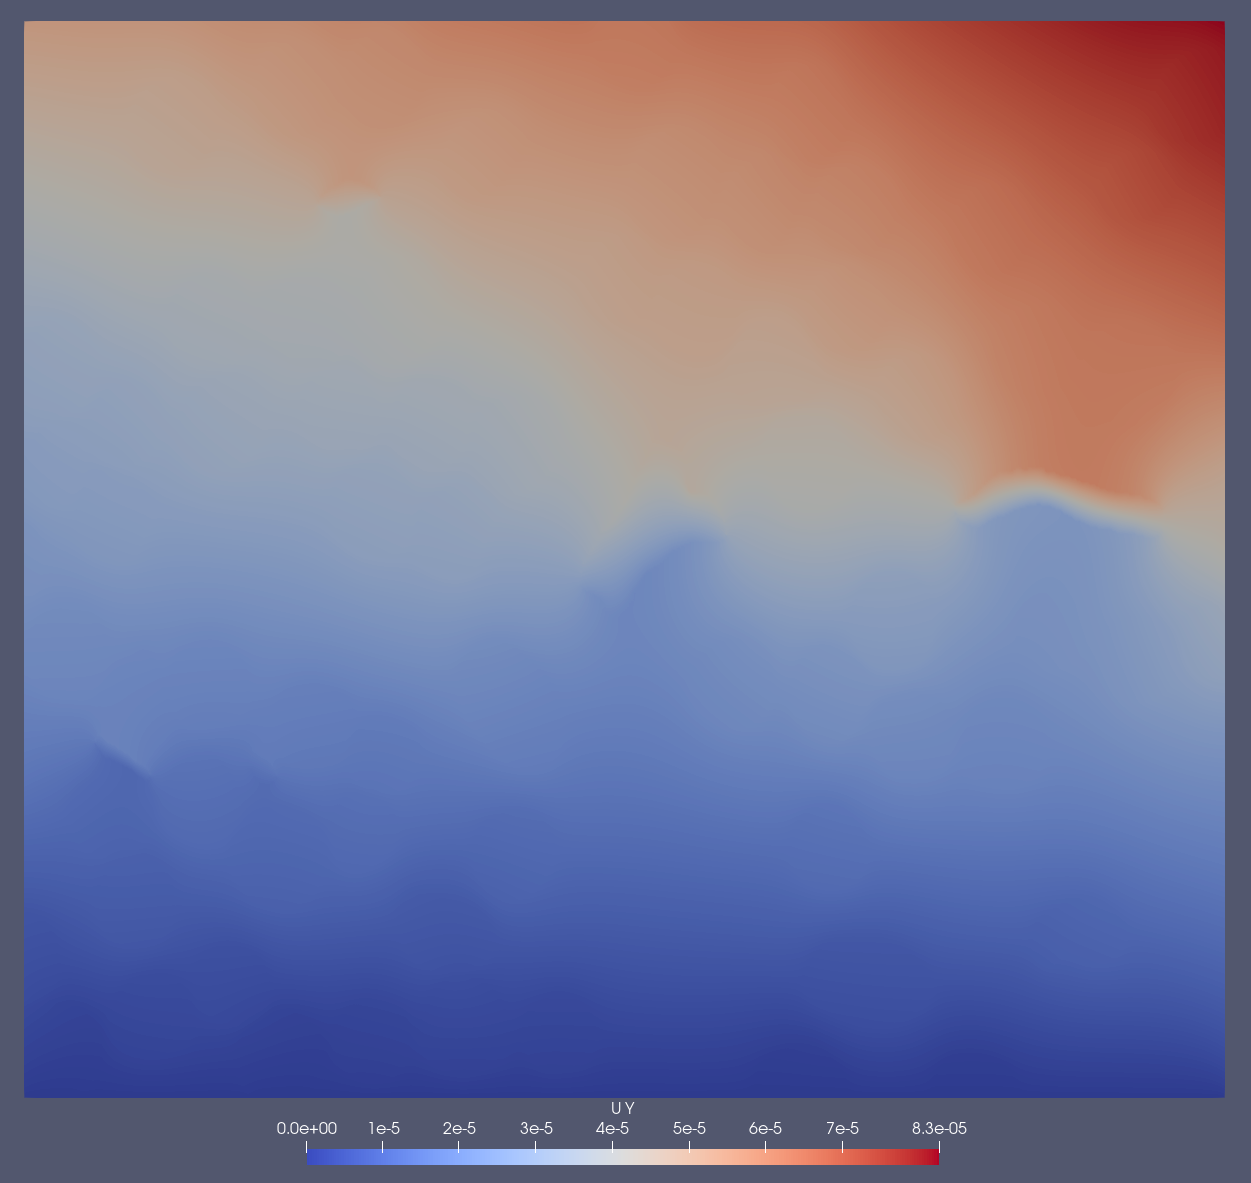
\includegraphics[width=0.49\textwidth]{figures/pores/uy_tracy.png}
    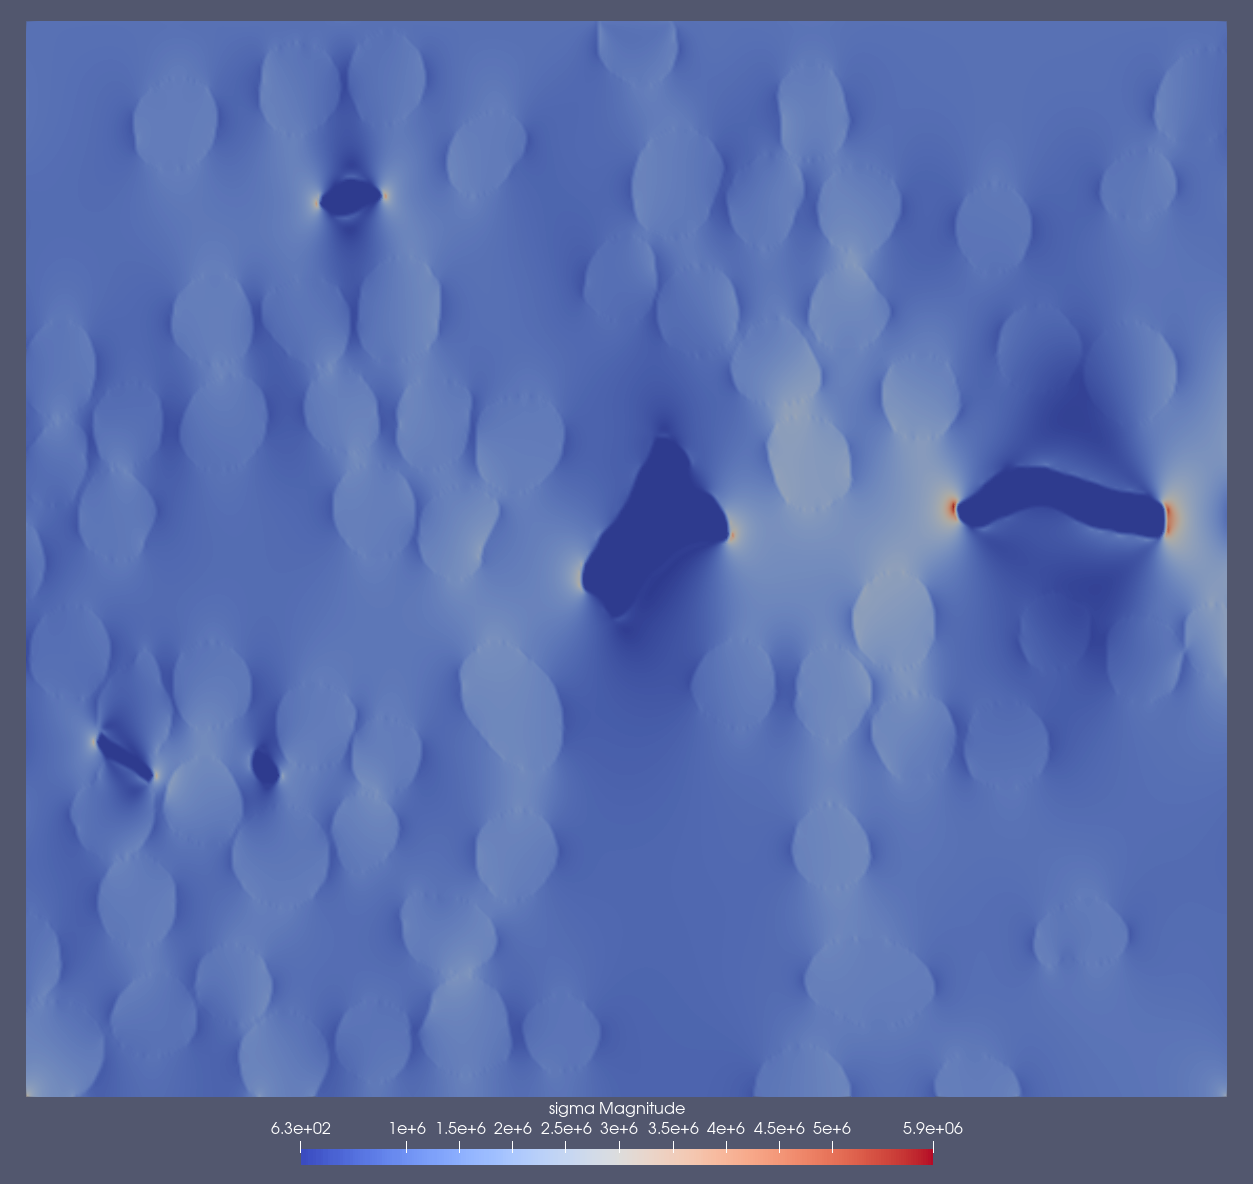
\includegraphics[width=0.49\textwidth]{figures/pores/sigmamag_ty.png}
    \caption{Champs de déplacement $u_y$ (gauche) et norme du champ de contrainte $\sigma_{\text{mag}}$ (droite) pour une simulation de traction dans la direction $y$ avec porosités.}
    \label{fig:pores_fields_tracy}
\end{figure}

Dans ce cas, on observe un comportement analogue, avec une forte hétérogénéité du champ de déplacement $u_y$, avec des zones de fractures autour des porosités, notamment celle ayant une dimension selon x plus importante que selon y. Cette porosité semble amplifier le déplacement dans tout le coin haut droit du domaine, ce qui est cohérent avec la nature du chargement. Concernant les contraintes, c'est principalement cette porosité qui génère des zones de forte concentration, dû à sa forme allongée perpendiculairement à la traction, avec des valeurs d'environ 5.9 MPa. Ces zones sont situées autour de la porosité, perpendiculairement à la direction de traction, tandis que les zones dans l'axe de la direction de traction montrent des contraintes beaucoup plus faibles comparé au reste du domaine. \\

L'étude des porosités montre clairement leur impact négatif sur les propriétés mécaniques du composite, avec une réduction significative du module d'Young et du module de cisaillement, ainsi que la création d'un comportement anisotrope dans le plan. Les champs de déplacement et de contrainte montrent des zones de forte hétérogénéité autour des porosités, avec des zones de concentration de contraintes pouvant atteindre plus de 6 fois le chargement appliqué, ce qui illustre l'importance de prendre en compte ces défauts dans la modélisation des composites C/C. Ces résultats sont cohérents avec la physique du problème et montrent que le code éléments finis est capable de capturer correctement l'impact des porosités sur les champs mécaniques.

\section{Homogénéisation numérique dans la direction longitudinale}

\subsection{Contexte et méthodologie}

La dernière approche manquante pour établir une loi de comportement macroscopique complète du composite C/C est l'homogénéisation numérique dans la direction longitudinale, c'est-à-dire en appliquant des conditions de traction selon la direction des fibres. Grâce à la segmentation U-Net, il est possible d'extraire des maillages à partir d'images 2D montrant des fibres en coupe orientées dans la direction longitudinale selon x. Le problème est que la fibre (et la matrice) n'est pas isotrope dans le plan de l'image contrairement à avant, car y correspond à la direction transverse de la fibre. Ci-dessous, nous présentons un exemple d'image et sa segmentation pour un VER avec des fibres longitudinales orientées selon x, qui correspond à une fraction volumique de fibre d'environ 0.6.

\begin{figure}[H]
    \centering
    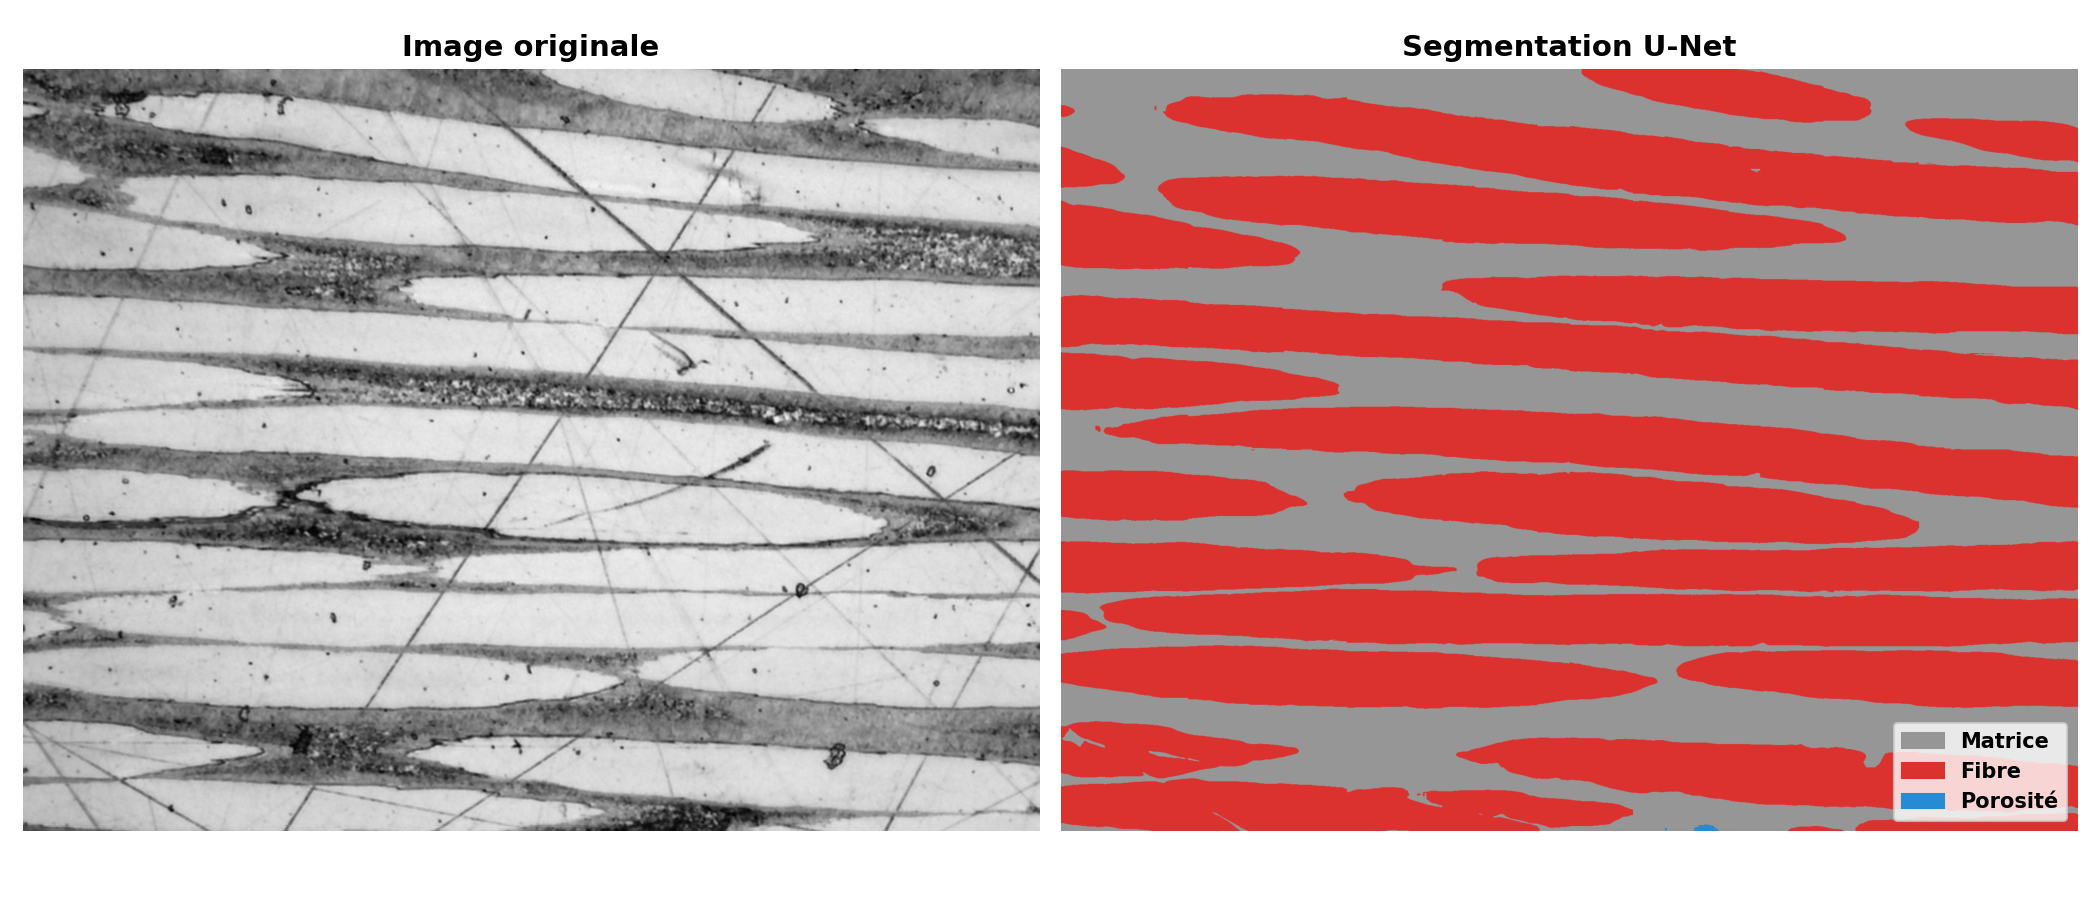
\includegraphics[width=0.9\textwidth]{figures/11_segmented.png}
    \caption{Fibres orientées selon x : image originale (gauche) et segmentation U-Net (droite).}
    \label{fig:segm_longitudinal}
\end{figure}
L'avantage de cette image est que l'on observe les fibres dans la direction longitudinale, avec une longueur bien plus importante que la largeur de la fibre. C'est une approximation car les fibres sont plus ou moins elliptiques sur cette image, mais l'on fera l'hypothèse que les fibres sont parfaitement rectangulaires, comme si l'on observait une coupe longitudinale d'une fibre. Un autre avantage est que ces fibres sont alignées avec l'axe x, ce qui facilitera l'essai de traction pour extraire les propriétés effectives dans la direction longitudinale. \\ 

Le code n'étant pas encore adapté pour traiter des matériaux anisotropes, il est nécessaire de faire une approximation en traitant la fibre et matrice comme isotropes dans le plan. Cela n'est pas vraiment car dans le repère de l'image, la fibre et matrice sont bien plus rigides selon x que selon y. Cette approximation grossière, permet d'avoir une première estimation des propriétés effectives au moins dans la direction longitudinale : $E_L$ et dans une moindre mesure $G_{LT}$ et $\nu_{LT}$. Il est tout de même possible de comparer les autres propriétés effectives obtenues dans le plan transverse, comme $E_T$ et $\nu_{TT}$ pour vérifier la cohérence (même si elles seront différentes de celles obtenues précédemment). \\

\subsection{Propriétés des constituants}
Pour les valeurs des propriétés de la fibre et de la matrice, nous utilisons des données issues de la littérature pour la direction longitudinale, qui sont différentes de celles utilisées pour le plan transverse. Pour la fibre, nous utilisons les valeurs pour la fibre PANEX 33 de chez Zoltek, présentée dans la partie théorique, tandis que pour la matrice, nous utilisons des propriétés de matrice Pyrocarbone Laminaire Lisse (LL), issu de la thèse de M. Charron \cite{CharronCC}, afin d'avoir un contraste fibre/matrice. Le tableau ci-dessous résume les propriétés utilisées dans ce plan d'étude : 

\begin{table}[H]
\centering
\small
\renewcommand{\arraystretch}{1.2}
\begin{tabular}{|c|c|c|}
\hline
\textbf{Phase} & \textbf{$E_L$} & \textbf{$\nu_{LT}$} \\
\hline
Fibre (PANEX 33)  & 228 GPa & 0,20 \\
Matrice (Pyrocarbone LL)& 54 GPa & 0,30 \\
\hline
\end{tabular}
\caption{Propriétés élastiques des constituants du composite pour les simulations.}
\label{tab:properties_longi}
\end{table}

\subsection{Résultats et interprétation}
Les propriétés effectives sont extraites de la même manière que pour le plan transverse, en appliquant des tractions dans la direction x pour obtenir $E_L$, et $\nu_{LT}$. Un cisaillement est aussi appliqué sur le bord droit pour extraire $G_{LT}$. L'essai selon y permet d'obtenir $E_T$ et $\nu_{TT}$, qui sont des propriétés effectives dans le plan transverse, à prendre avec précaution comme expliqué précédemment. Le tableau ci-dessous résume les propriétés effectives avec les bornes analytique de Voigt, Reuss, Hill et Halpin-Tsai ($\xi$ fixé à 8 ici) pour la direction longitudinale, en utilisant la fraction volumique de fibre d'environ 0.6 extraite du maillage.

\begin{table}[H]
    \centering
    \begin{tabular}{|l|c|c|c|c|c|}
        \hline
        & \textbf{Numérique} & \textbf{Voigt} & \textbf{Reuss} & \textbf{Hill} & \textbf{Halpin-Tsai ($\xi=8$)} \\
        \hline
        $E_L$ (GPa) & 146,31 & \multirow{2}{*}{158,94} & \multirow{2}{*}{100,05} & \multirow{2}{*}{129,49} & \multirow{2}{*}{145,88} \\
        $E_T$ (GPa) & 104,59 &  &  &  &  \\
        \hline
        $\nu_{LT}$ & 0,253 & \multirow{2}{*}{0,240} & \multirow{2}{*}{0,230} & \multirow{2}{*}{0,235} & \multirow{2}{*}{0,239} \\
        $\nu_{TL}$ & 0,183 &  &  &  &  \\
        \hline
        $G_{LT}$ (GPa) & 42,08 & 65,54 & 39,28 & 52,41 & 59,44 \\
        \hline
    \end{tabular}
    \caption{Comparaison des propriétés effectives issues de la simulation EF avec les bornes analytiques. Les bornes sont identiques pour les directions 1 et 2 et sont mutualisées.}
    \label{tab:results_longi}
\end{table}

Les résultats montrent que le module d'Young longitudinal $E_L$ est d'environ 146 GPa, ce qui est cohérent avec les propriétés de la fibre et de la matrice, on retrouve un comportement bien plus proche de la borne de Voigt que de Reuss, ce qui est logique car la fibre est très rigide dans la direction longitudinale. $E_L$ peut être modélisé précisément par Halpin-Tsai pour une valeur de $\xi = 8$, ce qui traduit d'une géométrie où les fibres sont très longues par rapport à leur largeur, ce qui est le cas dans cette image. \\

Les autres propriétés sont à prendre avec des pincettes car l'approximation d'isotropie dans le plan n'est pas du tout vérifiée, mais on retrouve une tendance similaire à celle du plan transverse, avec des propriétés effectives plus proches de la borne de Reuss que de Voigt, notamment pour $E_T$ et $G_{LT}$, ce qui est cohérent avec le fait que la matrice est plus influente dans ces directions. Il y a toujours un écart important pour les coefficients de Poisson, qui sont sous-estimés par les modèles analytiques.
La symétrie des tenseurs de souplesse est toujours vérifiée, ce qui est rassurant quant à la fiabilité des résultats, même avec l'approximation. \\

Cette étude d'homogénéisation permet au moins de compléter la loi de comportement macroscopique du composite C/C dans la direction longitudinale, notamment pour $E_L$, qui est une propriété essentielle pour la conception de structures en composite C/C. Cependant, il serait nécessaire d'adapter le code pour traiter des matériaux anisotropes afin d'obtenir des résultats plus précis pour les autres propriétés effectives. L'étude du champ de déformation et de contrainte permet aussi d'illustrer le comportement différent des fibres dans ce plan :

\begin{figure}[H]
    \centering
    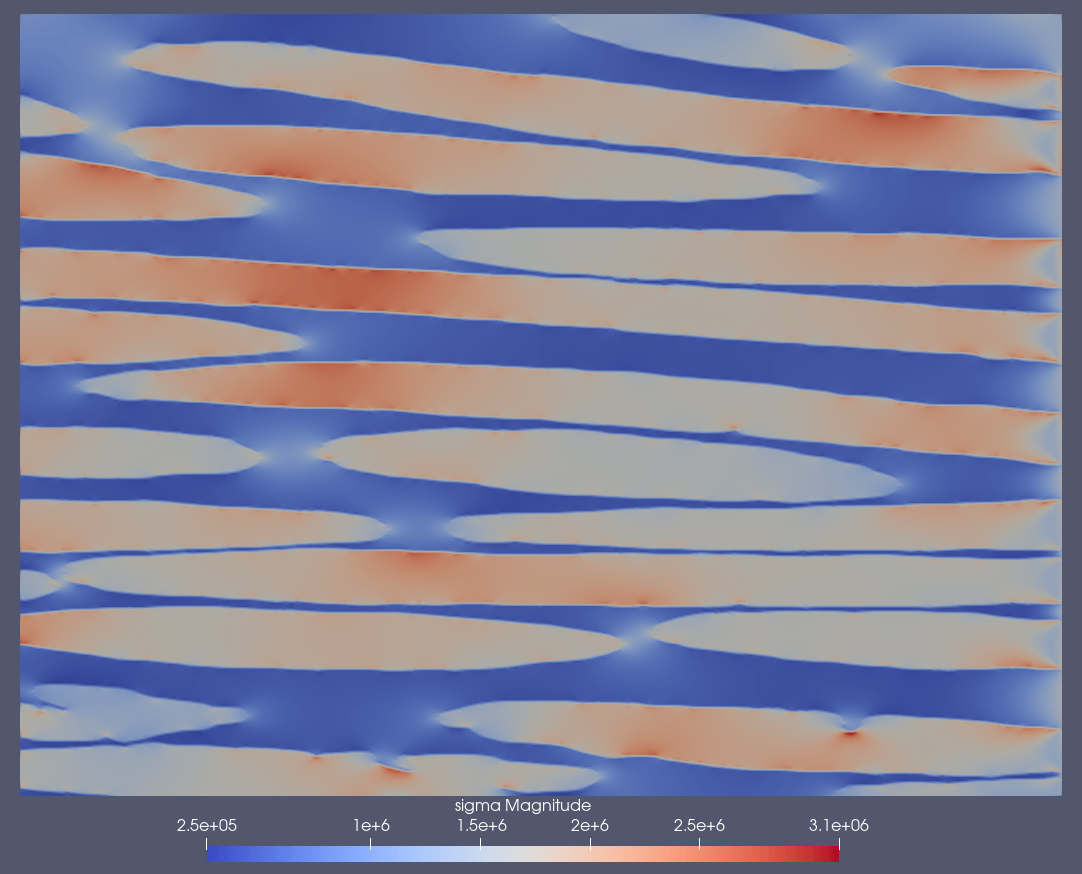
\includegraphics[width=0.49\textwidth]{figures/sigmamag_longi.png}
    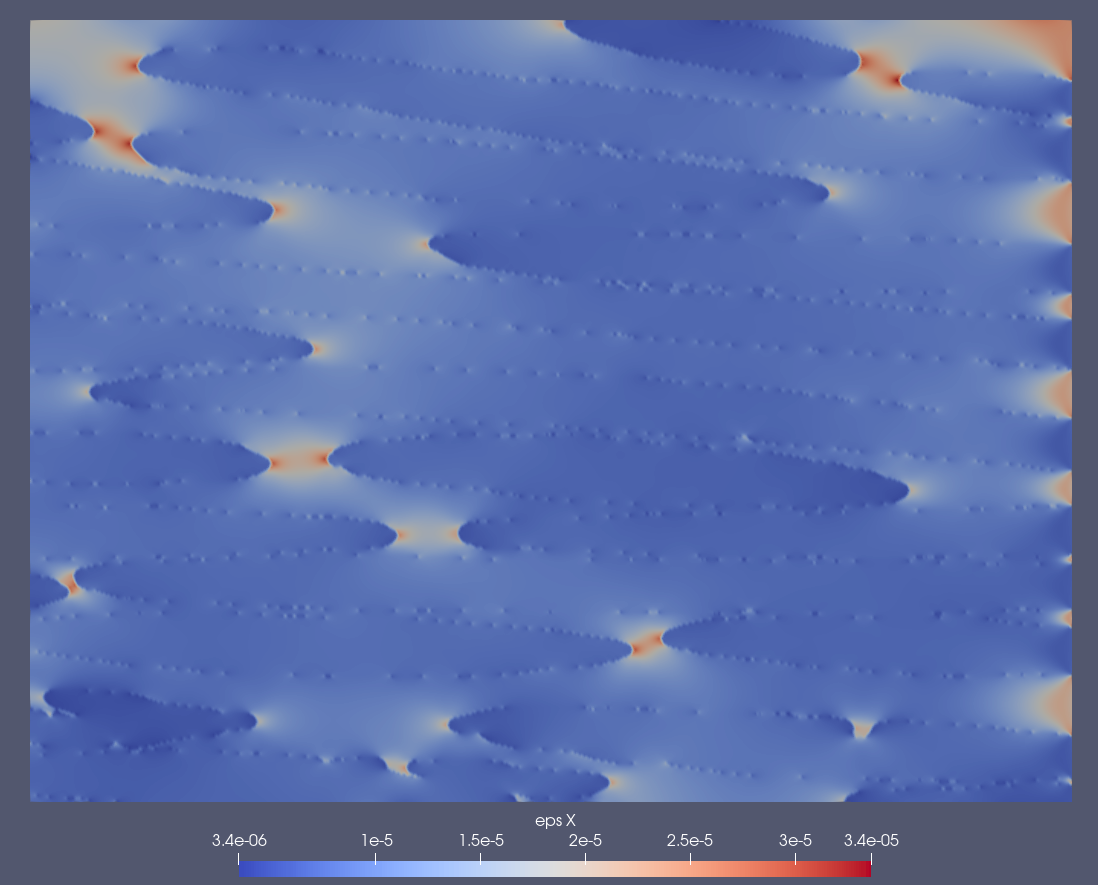
\includegraphics[width=0.49\textwidth]{figures/epsx_longi.png}
    \caption{Champ de norme de contrainte $\sigma_{\text{mag}}$ (gauche) et champ de déformation $\varepsilon_{xx}$ (droite) pour une simulation de traction dans la direction longitudinale.}
    \label{fig:longi_fields}
\end{figure}

Le champ de norme de contrainte montre une forte hétérogénéité, avec des zones de forte concentration de contraintes dans les fibres, tandis que la matrice montre des contraintes beaucoup plus faibles (10 fois moins élevées environ), ce qui est cohérent avec les propriétés des constituants. Le champ de déformation $\varepsilon_{xx}$ est plus homogène dans le domaine (hypothèse iso-déformation Reuss), mais on observe des zones de gradient plus important à l'interface fibre/matrice, ce qui est cohérent avec la nature du composite et les propriétés des constituants. Les remarques sont similaires à celles faites pour le plan transverse, avec des zones de forte hétérogénéité autour des fibres, et une bonne cohérence avec la physique du problème.

\newpage
\section*{Conclusion}
\addcontentsline{toc}{section}{Conclusion}

En conclusion, ce projet a permis de développer une méthodologie complète d'homogénéisation numérique pour un composite C/C à partir d'images microscopiques segmentées par un réseau de neurones U-Net. L'utilisation de deep learning pour la segmentation a permis d'obtenir des maillages de haute qualité, fidèles à la microstructure réelle du composite. La mise en oeuvre d'un code éléments finis en C++ pour l'élasticité linéaire a permis d'extraire les propriétés mécaniques effectives du composite dans les plans transverse et longitudinal, en appliquant des conditions aux limites appropriées. Ce solveur a été validé sur des cas tests analytiques, et sur des tests de convergence en maillage, montrant une bonne précision et robustesse. Les résultats obtenus pour les propriétés effectives dans les plans transverse et longitudinal sont cohérents avec la physique du problème et montrent l'importance de prendre en compte la microstructure réelle du composite pour obtenir des propriétés mécaniques précises. L'homogénéisation montre qu'un modèle analytique ajusté comme celui d'Halpin-Tsai peut capturer de manière très précise l'évolution des propriétés effectives en fonction de la fraction volumique de fibre, ce qui est très utile pour la conception de composites avec des propriétés mécaniques spécifiques. L'étude de l'influence des porosités a montré leur impact négatif significatif sur les propriétés mécaniques du composite, ainsi que la création d'un comportement anisotrope dans le plan. Enfin, l'homogénéisation dans la direction longitudinale a permis de compléter la loi de comportement macroscopique du composite C/C, ce qui ouvre la voie à une modélisation homogénisée à l'échelle macroscopique. \\ 

Cependant, il serait nécessaire d'adapter le code pour traiter des matériaux anisotropes afin d'obtenir des résultats plus précis pour les propriétés effectives dans les plans transverse et longitudinal. L'étude du comportement de rupture du composite, notamment en présence de porosités, serait aussi un sujet intéressant à explorer pour compléter la compréhension du comportement mécanique du composite C/C. Enfin, l'intégration d'une approche non linéaire pour l'élasticité et l'ajout d'un solveur thermomécanique permettraient d'obtenir une modélisation plus complète du composite C/C, notamment pour les applications à haute température.
\clearpage
\thispagestyle{empty}
\addcontentsline{toc}{section}{Références}
\begin{thebibliography}{99}
    
\footnotesize

\bibitem{SavageCCC}
G. Savage,
\textit{Carbon-Carbon Composites},
Chapman \& Hall.

\bibitem{ZienkiewiczFEM}
O. C. Zienkiewicz, R. L. Taylor,
\textit{The Finite Element Method},
Butterworth-Heinemann.

\bibitem{RonnebergerUNet}
O. Ronneberger, P. Fischer, T. Brox,
\textit{U-Net: Convolutional Networks for Biomedical Image Segmentation},
Medical Image Computing and Computer-Assisted Intervention (MICCAI), 2015.

\bibitem{HeMultiscale}
Dongze He, Yang Chen, Christian Breite, Mikhail Y Matveev, Léonard Turpin, et al..
\textit{Multiscale image-based modelling of composite materials}. International Materials Reviews, 2025.

\bibitem{CharronCC}
M. Charron,
\textit{Modélisation basée images du comportement thermomécanique de composite C/C},
Thèse de doctorat.

\bibitem{GuruprasadNanoindent}
T. S. Guruprasad, V. Keryvin, L. Charleux, J.-P. Guin, O. Arnould,
\textit{On the determination of the elastic constants of carbon fibres by nanoindentation tests}.

\bibitem{GotoCC}
K. Goto, H. Ohkita, H. Hatta, H. Iseki, Y. Kogo,
\textit{Tensile strength and creep behavior of carbon-carbon composites at elevated temperatures},
Japan Aerospace Exploration Agency / Tokyo University of Science.

\bibitem{OzcanCC}
Özcan et al. (2009),
\textit{Microstructure and elastic properties of individual components of C/C composites}.

\bibitem{WallHomog}
P. Wall,
\textit{A comparison of homogenization, Hashin-Shtrikman bounds and the Halpin-Tsai equations}.

\bibitem{CCOverview1}
\textit{An overview of carbon-carbon composite materials and their applications}.

\bibitem{RohiniCC}
G. Rohini Devi, K. Rama Rao,
\textit{Carbon-Carbon Composites: An Overview},
Defence Research and Development Laboratory, Hyderabad.

\bibitem{LUTSegmentation}
Lappeenranta–Lahti University of Technology LUT,
\textit{Deep Learning Segmentation of Fibre, Matrix, and Void Microstructure in Carbon Fibre and Flax Fibre Polymer Composites},
Master’s Thesis.

\bibitem{MaurinTransverseCC}
R. Maurin, P. Davies, N. Baral, C. Baley,
\textit{Transverse Properties of Carbon Fibres by Nano-Indentation and Micromechanics}

\bibitem{BertoldoUNet}
J. P. C. Bertoldo, E. Decencière, D. Ryckelynck, H. Proudhon,
\textit{A Modular U-Net for Automated Segmentation of X-Ray Tomography Images in Composite Materials}.

\bibitem{GillardCC}
A. P. Gillard, G. Couégnat, S. Chupin, G. L. Vignoles,
\textit{Modeling of the non-linear mechanical and thermomechanical behavior of 3D carbon/carbon composites based on internal interfaces}.

\bibitem{MLCarbon}
\textit{Elasticity of dense anisotropic carbons: A machine learning model of the structure–property relationship informed by large scale molecular dynamics data}.

\end{thebibliography}

\clearpage
\section*{Annexes}
\addcontentsline{toc}{section}{Annexes}
\appendix
\thispagestyle{empty}

\subsection*{Résultats des cas tests de validation}
\begin{table}[H]
    \centering
    \begin{tabular}{|c|c|c|c|c|c|}
        \hline
        $h$ & $n_{\text{elems}}$ & $\Delta W_{\text{rel}}$ & $\Delta E_{\text{rel}}$ & $\Delta \nu_{\text{rel}}$ & $t_{\text{cpu}}$ (s) \\
        \hline
        0,500000 & 4 & $2,13\times10^{-1}$ & $2,74\times10^{-1}$ & $9,59\times10^{-2}$ & $1,18\times10^{-5}$ \\
        0,250000 & 16 & $2,99\times10^{-2}$ & $9,99\times10^{-2}$ & $5,74\times10^{-2}$ & $2,53\times10^{-5}$ \\
        0,125000 & 64 & $6,59\times10^{-3}$ & $4,33\times10^{-2}$ & $2,90\times10^{-2}$ & $2,82\times10^{-4}$ \\
        0,062500 & 256 & $1,61\times10^{-3}$ & $2,05\times10^{-2}$ & $1,44\times10^{-2}$ & $7,66\times10^{-4}$ \\
        0,031250 & 1024 & $4,02\times10^{-4}$ & $1,00\times10^{-2}$ & $7,20\times10^{-3}$ & 0,78 \\
        0,015625 & 4096 & $1,00\times10^{-4}$ & $4,96\times10^{-3}$ & $3,62\times10^{-3}$ & 0,55 \\
        0,0078125 & 16384 & $2,51\times10^{-5}$ & $2,47\times10^{-3}$ & $1,82\times10^{-3}$ & 1,02 \\
        0,00390625 & 65536 & $6,27\times10^{-6}$ & $1,23\times10^{-3}$ & $9,10\times10^{-4}$ & 6,41 \\
        \hline
    \end{tabular}%
    \caption{Résultats de convergence pour le cas de traction simple.}
    \label{tab:validation_traction}
\end{table}

\begin{table}[H]
    \centering
    \begin{tabular}{|c|c|c|c|}
        \hline
        $h$ & $n_{\text{elems}}$ & $\Delta W_{\text{rel}}$ & $t_{\text{cpu}}$ (s) \\
        \hline
        0,100000 & 10 & $1,02\times10^{2}$ & $8,85\times10^{-5}$ \\
        0,050000 & 40 & $4,90\times10^{-1}$ & $5,88\times10^{-4}$ \\
        0,025000 & 160 & $9,91\times10^{-2}$ & $3,27\times10^{-3}$ \\
        0,012500 & 640 & $2,38\times10^{-2}$ & 0,29 \\
        0,006250 & 2560 & $5,93\times10^{-3}$ & 0,17 \\
        0,003125 & 10240 & $1,50\times10^{-3}$ & 1,05 \\
        0,0015625 & 40960 & $3,84\times10^{-4}$ & 11,51 \\
        0,00078125 & 163840 & $9,91\times10^{-5}$ & 92,60 \\
        \hline
    \end{tabular}%
    \caption{Résultats de convergence pour le cas de flexion.}
    \label{tab:validation_flexion}
\end{table}

\begin{table}[H]
    \centering
    \begin{tabular}{|c|c|c|c|}
        \hline
        $h$ & $n_{\text{elems}}$ & $\Delta W_{\text{rel}}$ & $t_{\text{cpu}}$ (s) \\
        \hline
        0,500000 & 4 & $2,61\times10^{-1}$ & $3,93\times10^{-5}$ \\
        0,250000 & 16 & $6,92\times10^{-2}$ & $1,13\times10^{-4}$ \\
        0,125000 & 64 & $1,93\times10^{-2}$ & $3,64\times10^{-4}$ \\
        0,062500 & 256 & $5,50\times10^{-3}$ & $1,57\times10^{-3}$ \\
        0,031250 & 1024 & $1,61\times10^{-3}$ & 0,30 \\
        0,015625 & 4096 & $4,86\times10^{-4}$ & 0,12 \\
        0,0078125 & 16384 & $1,51\times10^{-4}$ & 1,04 \\
        0,00390625 & 65536 & $4,82\times10^{-5}$ & 7,34 \\
        \hline
    \end{tabular}%
    \caption{Résultats de convergence pour le cas de cisaillement pur.}
    \label{tab:validation_shear}
\end{table}
\end{document}

\begin{table}[H]
    \centering
    \begin{tabular}{|l|c|}
        \hline
        \textbf{Propriétés} & \textbf{Valeur numérique} \\
        \hline
        $E_{11}$ & 18,1380 GPa \\
        $\nu_{12}$ & 0,28651 \\
        \hline
    \end{tabular}
    \caption{Propriétés effectives du cas de traction dans la direction $x$.}
    \label{tab:homo_traction_x}
\end{table}

\begin{table}[H]
    \centering
    \begin{tabular}{|l|c|}
        \hline
        \textbf{Propriétés} & \textbf{Valeur numérique} \\
        \hline
        $E_{22}$ & 18,0515 GPa \\
        $\nu_{21}$ & 0,28522 \\
        \hline
    \end{tabular}
    \caption{Propriétés effectives du cas de traction dans la direction $y$.}
    \label{tab:homo_traction_y}
\end{table}

\begin{table}[H]
    \centering
    \begin{tabular}{|l|c|}
        \hline
        \textbf{Propriétés} & \textbf{Valeur numérique} \\
        \hline
        $G_{12}$ & 7,1856 GPa \\
        \hline
    \end{tabular}
    \caption{Propriété effective du cas de cisaillement pur.}
    \label{tab:homo_shear}
\end{table}